\documentclass[11pt]{article}
\usepackage[T1]{fontenc}
\pdfinfoomitdate=1
\pdftrailerid{}
\pdfsuppressptexinfo=15
\usepackage{lmodern,microtype}
\usepackage[margin=1.05in]{geometry}
\usepackage{amsmath,amssymb,amsthm,mathtools,mathrsfs}
\usepackage{enumitem,booktabs,array,needspace}
\usepackage[numbers,sort&compress]{natbib}
\usepackage{xurl}
\usepackage{tikz}
\usetikzlibrary{arrows.meta,positioning}
\usepackage[hidelinks]{hyperref}
\usepackage[nameinlink,capitalize,noabbrev]{cleveref}
\hypersetup{pdftitle={Universal strong Kadison--Kastler stability},pdfauthor={OpenAI},pdfsubject={September 23, 2026},bookmarksdepth=2}
\setcounter{tocdepth}{2}
\allowdisplaybreaks[1]
\numberwithin{equation}{section}
\newtheorem{theorem}{Theorem}[section]
\newtheorem{lemma}[theorem]{Lemma}
\newtheorem{proposition}[theorem]{Proposition}
\newtheorem{corollary}[theorem]{Corollary}
\theoremstyle{definition}
\newtheorem{definition}[theorem]{Definition}
\newtheorem{remark}[theorem]{Remark}
\newcommand{\C}{\mathbb C}
\newcommand{\R}{\mathbb R}
\newcommand{\N}{\mathbb N}
\newcommand{\Z}{\mathbb Z}
\newcommand{\E}{\mathbb E}
\newcommand{\B}{\mathcal B}
\newcommand{\U}{\mathcal U}
\newcommand{\HH}{\mathcal H}
\newcommand{\KK}{d}
\newcommand{\dcb}{d_{\mathrm{cb}}}
\newcommand{\cb}{\mathrm{cb}}
\newcommand{\id}{\operatorname{id}}
\newcommand{\Ad}{\operatorname{Ad}}
\newcommand{\ad}{\operatorname{ad}}
\newcommand{\dist}{\operatorname{dist}}
\newcommand{\Tr}{\operatorname{Tr}}
\newcommand{\supp}{\operatorname{supp}}
\newcommand{\eps}{\varepsilon}
\newcommand{\norm}[1]{\lVert#1\rVert}
\newcommand{\abs}[1]{\lvert#1\rvert}
\newcommand{\ip}[2]{\langle #1,#2\rangle}
\newcommand{\barotimes}{\mathbin{\overline\otimes}}
\newcommand{\II}{\mathrm{II}}
\newcommand{\III}{\mathrm{III}}
\DeclareMathOperator{\RePart}{Re}
\DeclareMathOperator{\ImPart}{Im}

\title{Universal strong Kadison--Kastler stability}
\author{OpenAI}
\date{September 23, 2026}
\begin{document}
\maketitle
\begin{abstract}
We prove that sufficiently close unital von Neumann algebras are
conjugate by a unitary arbitrarily close to the identity. The tolerance
depends only on the prescribed distance of that unitary from the
identity, uniformly over all algebras, representations, and Hilbert
spaces. This resolves the strong Kadison--Kastler conjecture.
\end{abstract}
\tableofcontents
\section{Introduction}
\label{sec:introduction}

For a von Neumann algebra $M\subseteq\B(H)$, write $M_1$ for its
closed operator-norm unit ball. The Kadison--Kastler distance between
two such algebras is
\begin{equation}\label{eq:kk-definition}
 d(M,N)=\max\left\{
 \sup_{x\in M_1}\inf_{y\in N_1}\norm{x-y},\quad
 \sup_{y\in N_1}\inf_{x\in M_1}\norm{x-y}\right\}.
\end{equation}
Kadison and Kastler introduced this metric in 1972
\cite{KadisonKastler1972}. Their perturbation problem asks whether
closeness of the unit balls forces spatial isomorphism, implemented by
a unitary close to the identity. We prove the uniform form of this
assertion.

\begin{theorem}[Strong Kadison--Kastler stability]\label{thm:main}
For every $\eps>0$ there is $\delta=\delta(\eps)>0$ such that the
following holds. If $H$ is any complex Hilbert space and
$M,N\subseteq\B(H)$ are unital von Neumann algebras with identity
$I_H$ and $d(M,N)<\delta$, there is a unitary $u\in\B(H)$ satisfying
\[
 uMu^*=N,\qquad \norm{u-I_H}<\eps.
\]
\end{theorem}

The tolerance is independent of the algebras, their type, their
representations, and the cardinalities of their preduals and Hilbert
spaces. Thus \Cref{thm:main} resolves the strong Kadison--Kastler
conjecture positively. Its hypothesis concerns the ordinary distance
\eqref{eq:kk-definition}.

\subsection{Historical context}

Early positive results treated type~I algebras:
Phillips proved spatial isomorphism, and Christensen obtained a conjugating
unitary close to the identity \cite{Phillips1974,Christensen1975}.
The work of Christensen, Johnson, and Raeburn--Taylor established the
amenable case \cite{Christensen1977,Johnson1977,RaeburnTaylor1977}.
Christensen subsequently developed the one-sided theory of near inclusions:
an amenable von Neumann algebra sufficiently nearly contained in another
can be moved into it by a small unitary \cite{Christensen1980}.
His earlier work also treated close von Neumann subalgebras of a common
finite von Neumann algebra \cite{Christensen1977II}. The common finite
ambient algebra is an essential hypothesis of that result; merely assuming
that both represented algebras are finite gives a different problem.
In a different common-ambient setting, Ino proved near-identity unitary
conjugacy for sufficiently close subalgebras of a countably decomposable
ambient algebra when both admit conditional expectations of finite
probabilistic index from that algebra \cite[Theorem~3.2]{Ino2016}.

The corresponding development for $C^*$-algebras clarifies the role of the
conclusion. Christensen, Sinclair, Smith, White, and Winter proved that
sufficiently close $C^*$-algebras acting on a separable Hilbert space
are spatially isomorphic if one of them is norm separable and nuclear
\cite{CSSWW2010,CSSWW2012}.
Johnson's examples exclude a uniform bound on the displacement of an
implementing unitary that tends to zero with the algebra distance;
they do not exclude spatial isomorphism \cite{Johnson1982}.

For nonamenable von Neumann algebras, Cameron, Christensen, Sinclair, Smith,
White, and Wiggins constructed strongly stable factors of the form
$(L^\infty(X)\rtimes\mathrm{SL}_n(\mathbb Z))\barotimes R$, where
$n\geq3$, the action is free, ergodic, and probability preserving on a
standard nonatomic probability space, and $R$ is the hyperfinite
type~$\mathrm{II}_1$ factor \cite{CCSSWW2012,CCSSWW2014}.
Their proof combines amenable near-inclusion methods, a common standard
representation, and bounded cohomology. Their later work transfers
property~$\Gamma$ and Cartan structure between sufficiently close type
$\II_1$ factors with separable predual, and also studies stability of
solidity, strong solidity, and tensor-product structure
\cite{CCSSWW2017}.

The passage between representations is tied to Kadison's similarity
problem: whether a bounded homomorphism from a $C^*$-algebra into
$\B(H)$ is conjugate by an invertible operator to a $*$-homomorphism.
Christensen's work on property~$\Gamma$ factors provides a
foundational special case \cite{Christensen1986,Christensen2001}.
Christensen, Sinclair, Smith, and White established perturbation results
for the similarity property and operator-algebraic invariants
\cite{CSSW2010}; Cameron and collaborators then proved that the similarity
property is equivalent to continuity of commutants, with the required
uniformity over representations \cite{CCSSWW2013}.
These results explain why ordinary norm closeness, control at all matrix
levels, and implementation on the original Hilbert space must be kept
distinct throughout a proof of strong stability.
The companion manuscript \cite{OpenAI2026Similarity} also proves a
uniform commutator estimate, using invariant tensors and a free-corner
Hankel test. The amplification argument here instead uses free-word
randomization and is proved independently. Neither commutator estimate
alone constructs a nearby multiplicative correspondence between two
algebras; Appendix~\ref{app:comparison} compares their scope and this
remaining perturbation step.

The unit-ball metric supplies nearby elements but does not specify a
linear or multiplicative correspondence. We must construct such a
correspondence and control its implementation on the given Hilbert space,
with estimates independent of the algebras and representations.

\subsection{Proof overview}

We first work on separable Hilbert spaces. For finite factors, two
arguments meet in \Cref{sec:finite}. The first supplies matrix norm
control: for a separably acting type $\II_1$ factor $M\subseteq\B(H)$
and $h=h^*$, \Cref{thm:amplification} bounds all matrix amplifications
of $x\mapsto[h,x]$ by an absolute multiple of its ordinary operator
norm. It combines Haagerup's cyclic similarity estimate
\cite{Haagerup1983} and Popa's independence theorem for tracial
ultraproducts \cite{Popa2014} with a free-word randomization argument.
The constant is independent of matrix size and representation.

A separate argument constructs an isomorphism close in ordinary norm
to the inclusion. Using the common-position construction of
\cite[Lemma~4.10]{CCSSWW2014}, we move the factors to a tracial
representation in which one vector represents both traces, and the
left and right actions of a common hyperfinite subfactor $R$ agree.
The inclusion is irreducible, meaning $R'\cap M=\C I$.

For a countable strongly dense subgroup $G$ of the unitary group of $M$,
choose nearby unitaries $v_g\in N$. Their multiplication errors are
uniformly small. Section~\ref{sec:boundary} constructs a probability
space $D$ with an amenable $G$-action preserving null sets. An adaptation
of the averaging and polar-correction method for approximate
representations \cite{Kazhdan1982,BurgerOzawaThom2013} corrects the
nearby unitaries to measurable fields $W_g:D\to\U(N)$ satisfying
\[
 W_g(x)W_h(g^{-1}x)=W_{gh}(x).
\]
Here $G$ need not be amenable: the correction produces a cocycle over
its amenable action, not a representation on the original space.
On $D^2$, a tracial averaging argument and double ergodicity force a
suitable equivariant vector field to be constant. We give the
unitary-coefficient double-ergodicity argument in full, using the
bilateral random-walk viewpoint of Kaimanovich; Bj\"orklund gives
the corresponding unitary formulation and another proof
\cite{Kaimanovich2003,Bjorklund2014}. The resulting linear bijection preserves
adjoints and squares and is close to the inclusion; proximity excludes
reversal of multiplication. Transporting this isomorphism back and
applying the commutator estimate gives a small unitary on the original
Hilbert space.

For infinite factors, a common copy of $\B(\ell^2)$ identifies the
ordinary gap with the supremum of all matrix gaps. Tensoring with one
fixed hyperfinite factor gives type $\III_1$ factors with an
irreducible hyperfinite finite subfactor admitting a conditional
expectation. This preparation uses Marrakchi's absorption criterion
for a trivial bicentralizer and Haagerup's construction of the expected
hyperfinite subfactor \cite{Marrakchi2020,Haagerup1987}.
Houdayer and Marrakchi's September 2026 preprint proves triviality of
the bicentralizer for every type $\III_1$ factor with a faithful normal
state \cite[Theorem~G]{HoudayerMarrakchi2026}; the preparation here uses
only the earlier absorption criterion.

Small adjustments align the subfactor's left and right actions and
provide a common cyclic separating vector $\Omega$ whose two vector
states centralize $R$. For either algebra, the closure of
$x\Omega\mapsto x^*\Omega$ is its Tomita operator.
\Cref{prop:modular-graphs} shows that small matrix gaps force its two
graphs to be close when the output is multiplied by any $c>0$,
uniformly in $c$. This uniformity permits comparison of the modular
actions. A uniform infinitesimal estimate for type $\III$ factors
controls norm-continuous paths of unitaries whose conjugations nearly
preserve the algebra. Using Arveson's nest distance formula
\cite{Arveson1975}, analytic smoothing brings the modular comparison
into this setting. Limits of conjugation maps yield, at each time, a
unitary whose conjugation preserves one algebra and which is close to
the other algebra's modular unitary. Averaging corrects their
multiplication law. Section~\ref{sec:modular-alignment} thereby obtains
a single small change of position making the first algebra invariant
under that modular group.

We form crossed products using this common action. Their unit balls
are close at every matrix size, and continuous decomposition identifies
one crossed product as a type $\II_\infty$ factor
\cite{Takesaki1973,Takesaki2003II}. After aligning matrix units, its finite corner
and the corresponding nearby corner are both finite factors. The
finite-factor theorem conjugates these corners and hence the crossed
products. Averaging gives a unital completely positive (UCP) map between
the base algebras, meaning that it preserves the identity and positivity
at every matrix size. A state slice gives a second UCP map between the
original factors. The criterion in \Cref{prop:ucp}, derived from
Ricard--Roydor's multiplication perturbation theorem
\cite[Proposition~3.2]{RicardRoydor2014}, turns both maps into small
spatial isomorphisms. It does not require the averaging maps to be normal.

Finally, aligning centers and selecting measurable unitaries assembles
the factor results on separable spaces. For an arbitrary Hilbert space,
finite sets of operators and vectors lie in suitable separable
restrictions. Extend their small conjugating unitaries by the identity.
A subnet of the conjugation maps converges pointwise in the weak
operator topology to a UCP map. The finite tests put its range in the
required algebra, and the same criterion finishes the proof.
All tolerances depend only on the requested final unitary displacement.

\Cref{fig:proof} displays how the finite-factor result enters both the
finite and infinite cases and how they meet in the final reductions.

\begin{figure}[htbp]
\centering
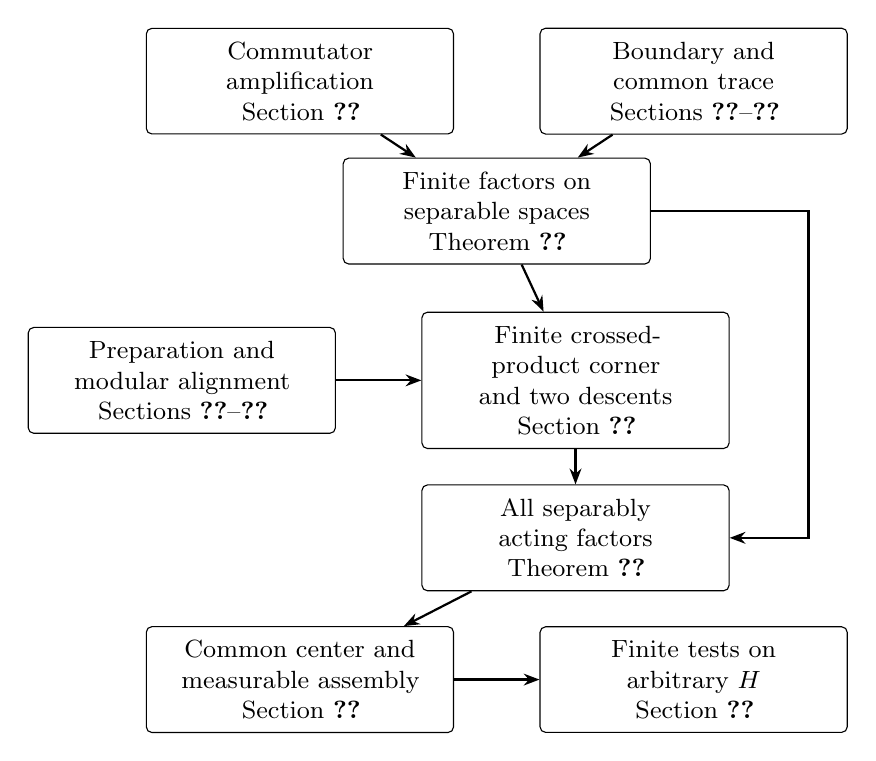
\begin{tikzpicture}[
 box/.style={draw,rounded corners=2pt,align=center,text width=3.55cm,
             minimum height=1.0cm,inner sep=5pt,font=\small},
 arr/.style={-{Stealth[length=2mm]},thick}]
 \node[box] (amp) at (-2.5,0) {Commutator amplification\\Section~\ref{sec:amplification}};
 \node[box] (boundary) at (2.5,0) {Boundary and common trace\\Sections~\ref{sec:boundary}--\ref{sec:finite}};
 \node[box] (finite) at (0,-1.65) {Finite factors on separable spaces\\Theorem~\ref{thm:finite}};
 \node[box] (modular) at (-4,-3.8) {Preparation and modular alignment\\Sections~\ref{sec:modular-preparation}--\ref{sec:modular-alignment}};
 \node[box] (corner) at (1,-3.8) {Finite crossed-product corner\\and two descents\\Section~\ref{sec:cores}};
 \node[box] (factors) at (1,-5.8) {All separably acting factors\\Theorem~\ref{thm:factors}};
 \node[box] (center) at (-2.5,-7.6) {Common center and\\measurable assembly\\Section~\ref{sec:reductions}};
 \node[box] (arbitrary) at (2.5,-7.6) {Finite tests on arbitrary $H$\\Section~\ref{sec:reductions}};
 \draw[arr] (amp)--(finite);
 \draw[arr] (boundary)--(finite);
 \draw[arr] (finite)--(corner);
 \draw[arr] (modular)--(corner);
 \draw[arr] (corner)--(factors);
 \draw[arr] (finite.east) -- ++(2.0,0) |- (factors.east);
 \draw[arr] (factors)--(center);
 \draw[arr] (center)--(arbitrary);
\end{tikzpicture}
\caption{The finite-factor theorem has two inputs and is reused in the
crossed-product argument. The UCP criterion supplies pointwise
normalizers in Section~\ref{sec:modular-alignment}, both descents in
Section~\ref{sec:cores}, and the final limit in Section~\ref{sec:reductions}.}
\label{fig:proof}
\end{figure}

Section~\ref{sec:foundations} proves the transfer tools.
Sections~\ref{sec:amplification}--\ref{sec:finite} establish the finite
case. Sections~\ref{sec:modular-preparation}--\ref{sec:cores} treat
infinite factors. Section~\ref{sec:reductions} removes the factor and
separability assumptions and gathers the final quantifiers.
Appendix~\ref{app:comparison} distinguishes uniformity over
representations from uniformity over factors and compares the
commutator methods of this paper and the similarity companion.

\newpage
\section{Perturbation tools and a completely positive criterion}
\label{sec:foundations}

Several steps of the proof produce an averaged map instead of a
homomorphism. The main result of this section, \Cref{prop:ucp}, turns
such a map into a small unitary conjugacy. All constants in this section
are independent of the algebras and Hilbert spaces.

\subsection{Metrics, amplification, and limits}

We use the unit-ball formula \eqref{eq:kk-definition} also for unital
$C^*$-algebras. For $A\subseteq\B(H)$, write $\U(A)$ for its unitary
group, $A'=\{T\in\B(H):Ta=aT\text{ for every }a\in A\}$ for its
commutant, and $Z(A)=A\cap A'$ for its center. The symbol
$A\barotimes B$ denotes the spatial von Neumann tensor product.

For a linear map $T:A\to\B(H)$, let $T_n$ act entrywise on $M_n(A)$,
and put $\norm{T}_{\cb}=\sup_n\norm{T_n}$.
The same notation for rectangular matrices is obtained by adding zero
rows and columns and compressing. For concretely represented von Neumann
algebras define
\[
 \dcb(A,B)=\sup_{n\ge1}d(M_n(A),M_n(B)).
\]
Here every matrix unit ball uses its operator norm on $H^n$.
We write $A\subset_\gamma B$ if there is $\gamma'<\gamma$ such that
every $x\in A_1$ has $\dist(x,B)\le\gamma'$; the approximant in $B$
need not be contractive. If $\norm{x}\le1$ and $\norm{x-y}\le r$, then
\[
 y_0=\frac{y}{\max\{1,\norm y\}}\in B_1,
 \qquad \norm{x-y_0}\le2r.
\]
We use this normalization whenever passing from near inclusions to
unit-ball distances. Conversely, a strict upper bound for $d(A,B)$
gives both near inclusions with that bound. For a unitary $v$,
\begin{equation}\label{eq:gap-adjustment}
 \begin{aligned}
 d(A,vBv^*)&\le d(A,B)+2\norm{v-I},\\
 \dcb(A,vBv^*)&\le\dcb(A,B)+2\norm{v-I}.
 \end{aligned}
\end{equation}
These inequalities follow at every matrix level from
$\norm{v_n x v_n^*-x}\le2\norm{v-I}\norm x$.
Also $\norm{v_1\cdots v_k-I}\le\sum_j\norm{v_j-I}$.

Inner products are linear in their first variable. A normal map between
von Neumann algebras is an ultraweakly continuous map. A map is
\emph{unital completely positive}, abbreviated UCP, if it preserves the
identity and each of its matrix amplifications is positive. Such maps
are completely contractive.

We repeatedly use the following elementary compactness facts. A bounded
operator ball is compact in the weak operator topology (WOT). A net of
UCP maps with fixed domain and codomain $\B(H)$ has a subnet converging pointwise in WOT:
use the product of the operator balls indexed by domain elements.
The limit is UCP, since linearity, the identity, and every finite matrix
positivity inequality pass to the limit. If the maps are within $a$ in
cb norm of a fixed map, so is their limit; apply WOT closedness of norm
balls at each fixed matrix size. If their values lie in a fixed von
Neumann algebra, the limit has the same property. Normality need not
pass to this limit and will not be required.

For clarity, $O(t)$ denotes a bound $Ct$ for an absolute constant $C$,
valid below an absolute positive threshold for $t$. Constants may change
between displays. A function tending to zero will always be chosen
uniformly over the explicitly stated class of algebras.

\subsection{The amenable embedding theorem}

The following form of Christensen's theorem supplies the small changes
of position used in the proof \cite{Christensen1980}.

\begin{theorem}[Amenable near inclusions]\label{thm:amenable}
Let $R,Q\subseteq\B(H)$ be von Neumann algebras with identity $I$, with
$R$ amenable. If $R\subset_\gamma Q$ and $\gamma<1/100$, there is a
unitary $v\in(R\cup Q)''$ such that
\[
 vRv^*\subseteq Q,\qquad \norm{v-I}\le150\gamma.
\]
If also $Q\subset_\gamma R$ and $\gamma<1/101$, the same conclusion
holds with $vRv^*=Q$.
\end{theorem}

This is \cite[Theorem~3.3(i)]{CCSSWW2014}, with its strict
near-inclusion convention. The location of $v$ in $(R\cup Q)''$ is
useful: any algebra commuting with both $R$ and $Q$ also commutes with
the change of position. We apply the theorem to abelian algebras,
hyperfinite finite factors, and type $\mathrm I$ algebras, all of which
are amenable.

\subsection{From commutators to intertwiners}

For $h\in\B(H)$ write $\ad_h(x)=[h,x]=hx-xh$.

\begin{lemma}\label{lem:commutant-cb}
For every unital von Neumann algebra $A\subseteq\B(H)$ and
$h\in\B(H)$,
\begin{equation}\label{eq:commutant-cb}
 \dist(h,A')\le\norm{\ad_h|_A}_{\cb}.
\end{equation}
Consequently $\dcb(A,B)\le\gamma$ implies $d(A',B')\le4\gamma$.
\end{lemma}

\begin{proof}
Since $A'$ is weak-star closed, its preannihilator in the trace class
computes the quotient norm $\dist(h,A')$. Let $\varphi$ be a trace-class
functional of norm at most one vanishing on $A'$. A singular-value
decomposition gives vectors $\xi,\eta\in\ell^2\otimes H$, each of
norm at most one, with
\[
 \varphi(x)=\ip{(I\otimes x)\xi}{\eta}\quad(x\in\B(H)).
\]
This uses only countably many vectors even when $H$ is nonseparable.
Let $p$ project onto $\overline{(I\otimes A')\xi}$. This subspace
reduces $I\otimes A'$, so every matrix entry of $p$ belongs to $A$.
Moreover $p\xi=\xi$ and $p\eta=0$. Therefore
\[
 \varphi(h)=\ip{[I\otimes h,p]\xi}{\eta}.
\]
If $q_n$ projects onto the first $n$ coordinates of $\ell^2$, the
compression of this commutator is
$[I_n\otimes h,q_npq_n]$, of norm at most
$\norm{\ad_h|_A}_{\cb}$ because $q_npq_n\in M_n(A)_1$.
Testing on finitely supported vectors and then using density proves
the same bound for the full commutator. Taking the supremum over
$\varphi$ proves \eqref{eq:commutant-cb}.

For $h\in A'_1$, approximate each contraction in $M_n(B)$ by one in
$M_n(A)$, with arbitrary slack above $\gamma$. It follows that
$\norm{\ad_h|_B}_{\cb}\le2\gamma$.
The first assertion gives distance at most $2\gamma$ to $B'$, and
normalization of approximants gives distance at most $4\gamma$ to
$B'_1$. Reverse the algebras to finish.
\end{proof}

\begin{lemma}[Close representations]\label{lem:paired}
Let $\rho,\theta:P\to\B(H)$ be normal unital $*$-representations of a
von Neumann algebra. If $\norm{\rho-\theta}_{\cb}\le e<1/4$, there
is a unitary $u\in\B(H)$ with
\[
 u\rho(x)u^*=\theta(x)\quad(x\in P),\qquad \norm{u-I}\le4e.
\]
\end{lemma}

\begin{proof}
If $e=0$, take $u=I$. Otherwise let
\[
 \pi(x)=\begin{pmatrix}\rho(x)&0\\0&\theta(x)\end{pmatrix},
 \qquad S=\begin{pmatrix}0&I\\I&0\end{pmatrix}.
\]
The von Neumann image $\pi(P)$ has the quotient matrix norms of $P$.
The commutator of $S$ with $\pi$ has cb norm at most $e$, hence the
same is true on $\pi(P)$ by quotient lifts with arbitrarily small
norm slack. By \Cref{lem:commutant-cb} choose $D\in\pi(P)'$ with
$\norm{D-S}<2e$. Its lower off-diagonal block $T$ satisfies
\[
 T\rho(x)=\theta(x)T,\qquad \norm{T-I}<2e<1.
\]
Thus $T$ is invertible and $T^*T$ commutes with $\rho(P)$.
Its polar unitary $u=T|T|^{-1}$ intertwines the representations.
The singular values of $T$ lie between $1-r$ and $1+r$, where
$r=\norm{T-I}$, so
\[
 \norm{u-I}\le\norm{u-T}+r=\norm{I-|T|}+r\le2r<4e.
\]
\end{proof}

\subsection{The completely positive criterion}

The norm relevant to perturbing a product is the completely bounded
norm on the Haagerup tensor product. We recall only the form needed
here. For a bilinear map $b:P\times P\to P$, it is the least $K$ such
that, at all rectangular sizes,
\begin{equation}\label{eq:haagerup-products}
 \left\|\left[\sum_{j=1}^r b(x_{ij},y_{jk})\right]_{i,k}\right\|
 \le K\norm X\norm Y,
 \quad X\in M_{p,r}(P),\quad Y\in M_{r,q}(P).
\end{equation}
Indeed the matrix Haagerup norm is the infimum of $\norm X\norm Y$
over such row-column factorizations. We write $\norm b_{\cb}$ for
this norm as well.

Write $m_P(x,y)=xy$ for the original multiplication on $P$.
Correction of multiplication by cohomological methods goes back to
Johnson and Raeburn--Taylor
\cite{Johnson1977,RaeburnTaylor1977}. We use the completely bounded
version supplied by Ricard--Roydor's multiplication perturbation theorem
\cite[Proposition~3.2]{RicardRoydor2014}: on a von Neumann algebra $P$,
an associative product $m$ with
$\norm{m-m_P}_{\cb}\le1/11$ admits a cb linear isomorphism $L$ with
\[
 L(m(x,y))=L(x)L(y),\qquad
 \norm{L-\id}_{\cb}\le10\norm{m-m_P}_{\cb}.
\]
If $m(x,y)^*=m(y^*,x^*)$, $L$ can preserve the involution.
There is no normality or separability assumption on the new product.

\begin{proposition}[UCP criterion]\label{prop:ucp}
Let $P,Q$ be von Neumann algebras, let
$\rho:P\to\B(H)$ be a faithful normal unital representation, and let
$Q\subseteq\B(H)$ have the same identity. Suppose that $F:P\to Q$ is
UCP and
\[
 \norm{F-\rho}_{\cb}\le e<10^{-3},\qquad
 \sup_{y\in Q_1}\dist(y,\rho(P)_1)\le g,\qquad g+e<1.
\]
Then there is a normal unital $*$-isomorphism $\theta:P\to Q$ and a
unitary $u\in\B(H)$ such that
\[
 \norm{\theta-\rho}_{\cb}\le32e,\qquad
 u\rho(x)u^*=\theta(x)\ (x\in P),\qquad \norm{u-I}\le128e.
\]
The map $F$ need not be normal.
\end{proposition}

\begin{proof}
Complete isometry of $\rho$ gives
$\norm{F_n(X)}\ge(1-e)\norm X$ at every matrix size. Thus $F$ is
injective, its range $V$ is norm closed, and
$\norm{F^{-1}:V\to P}_{\cb}\le(1-e)^{-1}$.
For $y\in Q_1$, match $y$ with $\rho(x)$ for $x\in P_1$, allowing
arbitrary slack, to obtain $\dist(y,V)\le g+e<1$.
If $V$ were proper, the quotient map $Q\to Q/V$ would have norm one,
contradicting this bound on $Q_1$. Hence $F$ is onto.

Transport multiplication from $Q$ to $P$:
\[
 m(x,y)=F^{-1}(F(x)F(y)).
\]
It is associative and preserves the involution. For rectangular $X,Y$,
insert $\rho(XY)=\rho(X)\rho(Y)$ to see that
\[
 \norm{F(XY)-F(X)F(Y)}\le3e\norm X\norm Y.
\]
Here the first difference is bounded by $e\norm{XY}$ and the product
difference by $2e\norm X\norm Y$, since $F$ and $\rho$ are complete
contractions. Equation~\eqref{eq:haagerup-products} therefore gives
\[
 q:=\norm{m-m_P}_{\cb}\le\frac{3e}{1-e}<\frac1{11}.
\]
The cited theorem gives an involution-preserving $L$ with
$\norm{L-\id}_{\cb}\le\lambda:=30e/(1-e)<1$.
Then $\theta=FL^{-1}$ is a bijective $*$-homomorphism, and
\[
 \norm{\theta-\rho}_{\cb}
 \le e+\norm{L^{-1}-\id}_{\cb}
 \le e+\frac{\lambda}{1-\lambda}
 = e+\frac{30e}{1-31e}\le32e.
\]
Bijective multiplicativity makes $\theta$ unital. A $*$-isomorphism
between von Neumann algebras is an order isomorphism on their
selfadjoint parts, so it preserves bounded increasing suprema and is
normal. Apply \Cref{lem:paired}, since $32e<1/4$.
When $e=0$, the preceding range argument gives $Q=\rho(P)$ directly.
\end{proof}

We will use this criterion both to descend from a tensor product and
to replace a pointwise weak limit by a spatial isomorphism. Its
quantitative conclusion depends only on the cb error of the map;
the ordinary reverse gap supplies surjectivity.

\subsection{Tensor products and averaging}

\begin{lemma}\label{lem:tensor-gap}
Let $A,B\subseteq\B(H)$ be unital von Neumann algebras with
$\dcb(A,B)\le\gamma$. If $K$ is separable, then
\[
 \dcb(A\barotimes\B(K),B\barotimes\B(K))\le\gamma.
\]
If $D\subseteq\B(K)$ is a von Neumann algebra whose commutant is the
strong closure of increasing finite-dimensional unital algebras, then
\[
 \dcb(A\barotimes D,B\barotimes D)\le\gamma.
\]
\end{lemma}

\begin{proof}
Compress a contraction of $M_n(A\barotimes\B(K))$ by increasing
finite-rank projections on $K$. In a corner of rank $r$, choose an
opposite contraction in $M_{nr}(B)$ within $\gamma$ plus arbitrarily
small slack, and extend it by zero on the complement. The compressions
of the original contraction converge strongly to it. A bounded WOT
cluster of the opposite contractions is in $M_n(B\barotimes\B(K))_1$
and is within $\gamma$, by WOT closedness of the norm bound, choosing
the approximation slack to tend to zero along the compressions. Reverse
the argument and take the supremum over $n$.

Now start with a contraction in $M_n(A\barotimes D)$. The first
assertion supplies a nearby contraction in
$M_n(B\barotimes\B(K))$. Average it by conjugation over the unitary
group of each finite-dimensional stage of $D'$. The input commutes
with these groups, so the bound is preserved. A WOT cluster of the
averages commutes with $D'$ and still lies in
$M_n(B\barotimes\B(K))$. The von Neumann tensor commutation theorem
\cite[Theorem~III.4.5.8 and Corollary~III.4.5.9, pp.~319--320]{BlackadarOperatorAlgebras}
places it in $M_n(B\barotimes D)$. Reverse and amplify as before.
\end{proof}

\begin{lemma}[Invariant operator means]\label{lem:invariant-mean}
Let $G$ be a discrete amenable group and $m$ a left invariant mean on
$\ell^\infty(G)$: thus $m$ is a positive unital linear functional with
$m(f(h^{-1}\,\cdot))=m(f)$ for every $h\in G$.
For a bounded family $T_g\in\B(K)$, define
\[
 \ip{(m_gT_g)\xi}{\eta}=m_g\ip{T_g\xi}{\eta}.
\]
This averaging map from bounded operator families to $\B(K)$ is UCP,
commutes with multiplication on either side by a fixed operator, and
preserves weak-operator closed linear subspaces. If
$\norm{T_g-T}\le a$ for every $g$, then
$\norm{m_gT_g-T}\le a$, also at rectangular matrix levels.
No measurability of the family is required.

For a unitary representation $g\mapsto V_g$ on $K$, the map
\[
 E_V(T)=m_gV_gTV_g^*\qquad(T\in\B(K))
\]
is a UCP projection onto $\{V_g:g\in G\}'$. It preserves every von
Neumann algebra invariant under these conjugations.
More generally, for an action by automorphisms $\alpha_g$ on a von
Neumann algebra $P$, the formula
\[
 \varphi(E(x))=m_g\varphi(\alpha_g(x))\qquad(\varphi\in P_*)
\]
defines a UCP map onto $P^G$ fixing that algebra. These averaging maps
need not be normal.
\end{lemma}

\begin{proof}
The coefficient formula defines a bounded sesquilinear form and hence
an operator. Positivity at every matrix size and unitality follow by
applying the positive scalar mean to matrix quadratic forms; the domain
has the pointwise operations on bounded operator families. Fixed left
and right factors pass through the coefficient formula. Testing the
linear equations defining a weak-operator closed subspace proves range
preservation. Testing vector coefficients at each rectangular size
gives the norm bound. For the action average, left invariance makes
the range invariant, while averaging fixes each invariant operator.
An invariant algebra is preserved by the preceding range property.
Predual duality gives the same argument for the general action on $P$,
including preservation of matrix norm bounds.
\end{proof}

For $G=\R$ with the discrete topology, an invariant mean is obtained
as a weak-star cluster point of uniform averages on finite boxes in
finitely generated subgroups. Direct the choices by a finite set of
translations and an error tolerance. Each subgroup is free abelian,
and the relative boundary of its boxes tends to zero for every
prescribed translation; the cluster is therefore positive, unital,
and translation invariant.

The boundary means in \Cref{sec:boundary} require a separate
construction: their equivariance involves a nonsingular action and
their module coefficients vary over the boundary space.

\section{Uniform amplification of commutators}
\label{sec:amplification}

The finite-factor argument will first produce an isomorphism that is close
to the given representation in operator norm. To implement it by a small
unitary, we need the same control at every matrix level. The following
estimate supplies that passage.

\begin{theorem}[Uniform amplification]\label{thm:amplification}
There is an absolute constant \(C_{\mathrm{amp}}\) such that, for every
type \(\II_1\) factor \(M\subseteq\B(H)\) on a separable Hilbert space and
every selfadjoint \(h\in\B(H)\),
\[
 \norm{\ad_h|_M}_{\cb}\le
 C_{\mathrm{amp}}\norm{\ad_h|_M}.
\]
The constant is independent of \(M\), its representation, and \(H\).
\end{theorem}

We first control columns by the cyclic similarity theorem. A free-word
estimate then permits us to apply this column bound to randomized matrix
coefficients. The randomization also recovers a fixed positive multiple
of the identity in a weak limit; this will detect every matrix
commutator. The auxiliary matrix sizes depend on the matrix level being
tested, but every estimate that survives to the conclusion is absolute.

\subsection{Columns and trace limits}

For \(a_1,\ldots,a_l\in\B(H)\), write
\(\norm{(a_i)_i}_{\mathrm{col}}=\norm{\sum_i a_i^*a_i}^{1/2}\).

\begin{lemma}[Column estimate]\label{lem:column-commutator}
Let \(A\subseteq\B(H)\) be a unital \(C^*\)-algebra, let \(h\in\B(H)\),
and put \(\delta=\norm{\ad_h|_A}\). Then
\[
 \norm{([h,a_i])_i}_{\mathrm{col}}
 \le 8\delta\,\norm{(a_i)_i}_{\mathrm{col}}
 \qquad(a_1,\ldots,a_l\in A).
\]
\end{lemma}

\begin{proof}
There is nothing to prove if \(\delta=0\). Otherwise
we use the triangular homomorphism associated with a derivation,
as in \cite[p.~216]{Haagerup1983}:
\[
 \Phi(a)=
 \begin{pmatrix}a&\delta^{-1}[h,a]\\0&a\end{pmatrix}
 \quad(a\in A).
\]
This is a unital homomorphism with \(\norm{\Phi}\le2\). For \(\xi\in H\),
the closed subspace
\[
 K_\xi=\overline{\{\Phi(a)(0,\xi):a\in A\}}
 \subseteq H\oplus H
\]
is invariant for \(\Phi(A)\), and the restricted homomorphism is cyclic.
Haagerup's cyclic similarity theorem gives
\(\norm{\Phi|_{K_\xi}}_{\cb}\le\norm{\Phi|_{K_\xi}}^3\le8\);
see \cite[Theorem~1.1 and its proof, pp.~217, 225]{Haagerup1983}.
Apply its column amplification to \((0,\xi)\in K_\xi\), and retain the
upper component of each output. This gives
\[
 \left(\sum_i\norm{[h,a_i]\xi}^2\right)^{1/2}
 \le8\delta\,\norm{(a_i)_i}_{\mathrm{col}}\norm{\xi}.
\]
Taking the supremum over unit vectors proves the claim.
\end{proof}

We use normalized traces on finite factors and the standard comparison
and subdivision of projections by trace
\cite[III.1.7.9--10, p.~257; III.2.5.4(iii) and Theorem~III.2.5.7,
p.~279]{BlackadarOperatorAlgebras}.
For a finite von Neumann
algebra \((P,\tau)\), put
\(\norm{x}_2=\tau(x^*x)^{1/2}\) and
\(\norm{x}_1=\tau(|x|)\). Fix a free ultrafilter \(\omega\) on
\(\N\). The tracial ultrapower \(P^\omega\) is the quotient of the
bounded sequences in \(P\) by those with
\(\lim_{j\to\omega}\norm{x_j}_2=0\); its trace is
\(\tau_\omega((x_j)_\omega)=\lim_{j\to\omega}\tau(x_j)\).
We identify \(P\) with its constant sequences.

\begin{lemma}[Transfer from the trace to a normal representation]
\label{lem:trace-transfer}
Let \(P\subseteq\B(K)\) be a finite von Neumann algebra with faithful
normal trace \(\tau\).
\begin{enumerate}[label=\textup{(\roman*)}]
\item If \((x_j)\) is bounded and
\(\lim_{j\to\omega}\norm{x_j}_2=0\), then
\(\lim_{j\to\omega}\norm{x_j\xi}=0\) for every \(\xi\in K\).
\item If \(x=(x_j)_\omega\in P^\omega\), then the weak-operator
ultralimit of \(x_j\) in this representation is \(E_P(x)\), where
\(E_P:P^\omega\to P\) is the trace-preserving conditional expectation.
\end{enumerate}
\end{lemma}

\begin{proof}
The functionals \(a\mapsto\tau(ba)\), \(b\in P\), are norm dense in
the predual \(P_*\). Indeed, their annihilator in
\((P_*)^*=P\) is zero, by faithfulness of the trace, so
Hahn--Banach gives the density.
For a normal vector functional \(\varphi\), approximate \(\varphi\)
in norm by one of these functionals. If \(\norm{x_j}\le K_0\), then
\[
 |\varphi(x_j^*x_j)|
 \le K_0^2\norm{\varphi-\tau(b\,\cdot)}
       +\norm{b}\norm{x_j}_2^2.
\]
This proves (i). For (ii), the defining identity of the conditional
expectation gives
\[
 \lim_{j\to\omega}\tau(bx_j)
 =\tau_\omega(bx)=\tau(bE_P(x))\qquad(b\in P).
\]
The same predual-density argument, using boundedness, extends the
identity to every normal functional.
\end{proof}

\subsection{Free projection words}

The following estimate controls sums of projection words whose labels have
the same multiplicities. In the later randomization, these sums will give
coefficients to which we apply the column estimate separately. When the
squared estimates are added, each diagonal vector component is counted
once for every multiset containing its label. We therefore need squared
word-norm bounds with a uniformly bounded sum through each fixed label.

\begin{lemma}[Free projection words]\label{lem:free-words}
For every integer $r\geq 1$ there are constants $C_r>0$ and an integer
$d_r\geq r$ with the following property.  Let $d\geq d_r$, and let
$(\mathcal A,\tau)$ be a von Neumann algebra with a faithful normal
tracial state.  Suppose that $A_1,\ldots,A_r\subset\mathcal A$ are
unital copies of $M_d(\C)$ which are scalar free: the trace of a product
of centered letters from successively different copies is zero.
For each $j$, let $(e_a^{(j)})_{a=1}^d$ be the diagonal minimal
projections of $A_j$.

For a multiset $W$ of cardinality $r$ drawn from $\{1,\ldots,d\}$, put
\[
 B_W=\sum_{\substack{(a_1,\ldots,a_r)\in\{1,\ldots,d\}^r\\
                     \text{with multiset }W}}
       e_{a_r}^{(r)}\cdots e_{a_1}^{(1)}.
\]
Then $\norm{B_W}\leq\beta_W$, where
\begin{equation}\label{eq:fw-beta}
 \beta_W=
 \begin{cases}
  7\sqrt{(r-1)!}\,d^{-(r-1)/2},
       &\text{if all labels in $W$ are distinct},\\
  C_r d^{-(r-1)/2},&\text{otherwise}.
 \end{cases}
\end{equation}
The constants and threshold depend only on $r$, not on the ambient
algebra, the free copies, or $W$.
\end{lemma}

Every word in $B_W$ ends with a projection $e_a^{(1)}$ whose label
occurs in $W$. Thus $B_W$ has right support in the sum of those
projections from the first copy, at most $r$ of them. This support
bound will let us reduce each coefficient to a column, once the
auxiliary matrix dimension is large enough.

\begin{proof}
We estimate the centered words first, then restore their scalar parts.
The decomposition below uses the creation, annihilation, and diagonal
actions in the free-product Hilbert space, as in the framework developed by
Voiculescu \cite{Voiculescu1985} and the reduced-free-product inequalities of
Ricard and Xu \cite[Section~1 and Fact~2.6]{RicardXu2006}.
The corresponding bound for words of fixed length in free groups is
Haagerup's inequality \cite[Lemma~1.4]{Haagerup1979}.
Here the prescribed label multiplicities require the additional tuple-matrix
and square-summation estimates proved below.

\paragraph{Reduced words and their cuts.}
We first describe the Hilbert space on which the word norm will be
estimated.  Replace $\mathcal A$ by $W^*(A_1,\ldots,A_r)$ and use its
faithful left representation on $L^2(\mathcal A,\tau)$.  Set
\[
 H_j^\circ=L^2(A_j,\tau)\ominus\C1.
\]
Freeness identifies this representation space with
\begin{equation}\label{eq:fw-fock}
 \mathcal F=\C\Omega\ \oplus\!
 \bigoplus_{\substack{\ell\geq1,\ i_1,\ldots,i_\ell\in\{1,\ldots,r\}\\
                      i_t\ne i_{t+1}}}
 H_{i_1}^\circ\otimes\cdots\otimes H_{i_\ell}^\circ.
\end{equation}
Indeed, map a tensor to the corresponding product applied to $1$.
Its inner products are the tensor inner products: in the trace of the
adjoint of one reduced word times another, pair the adjacent letters
at the junction, split their product into its trace and centered part,
and iterate.  Freeness eliminates the centered terms until the copy
sequences agree and all letters have been paired.  Distinct summands
are orthogonal.  Splitting each letter into its scalar and centered
parts shows that reduced words span the algebra generated by the
copies, hence a dense subspace of $L^2(\mathcal A,\tau)$.

Write $h_a^{(j)}=e_a^{(j)}-d^{-1}1$.  Define the label map
\[
 D_j:\ell^2(\{1,\ldots,d\})\longrightarrow H_j^\circ,
 \qquad D_j\delta_a=h_a^{(j)}.
\]
The normalized matrix trace gives
\begin{equation}\label{eq:fw-label-map}
 D_j^*D_j=\frac1d I-\frac1{d^2}\mathbf1\mathbf1^*,
 \qquad \norm{D_j}\leq d^{-1/2},
\end{equation}
where $\mathbf1$ is the vector all of whose entries are one.

Left multiplication by $h_a^{(j)}$ creates the first letter
$h_a^{(j)}$ on a reduced tensor not beginning in copy $j$.
On a tensor $b\otimes\xi$ beginning in that copy, it has two parts:
annihilation, equal to $\tau(h_a^{(j)}b)\xi$, and preservation of the
first leg, with operator
\begin{equation}\label{eq:fw-preservation-operator}
 K_a^{(j)}
 =P_j^\circ L_{e_a^{(j)}}P_j^\circ
       -\frac1d I_{H_j^\circ}
 \quad\text{on }H_j^\circ.
\end{equation}
Here $P_j^\circ$ is the orthogonal projection onto $H_j^\circ$ inside
$L^2(A_j,\tau)$, and $L$ denotes left multiplication.  These formulas
also apply to the vacuum, on which only creation occurs.

Consider a fully centered word
$h_{a_r}^{(r)}\cdots h_{a_1}^{(1)}$.  The rightmost letter acts first.
Since the copy indices $1,\ldots,r$ are distinct, once a creation or
preservation occurs, every later operation must be a creation.
Thus the word is a sum of cuts of two kinds: $p$ annihilations followed
by $q=r-p$ creations, or $p$ annihilations, one preservation, and
$q=r-p-1$ creations.

For completeness, the domain restrictions in these cuts can be made
explicit.  For a set $S$ of copy indices, let $\mathcal F_{\notin S}$
denote the vacuum plus all reduced tensors whose first copy index is
outside $S$.  For a cut without preservation put
\[
 S_p=\bigl(\{p\}\text{ if }p\geq1\bigr)
       \cup\bigl(\{p+1\}\text{ if }p<r\bigr),
 \qquad E_p=\mathcal F_{\notin S_p}.
\]
Its source and target spaces are canonically embedded copies of
\[
 H_1^\circ\otimes\cdots\otimes H_p^\circ\otimes E_p,
 \qquad
 H_r^\circ\otimes\cdots\otimes H_{p+1}^\circ\otimes E_p,
\]
respectively; empty tensor products mean $\C$.  Excluding copy $p$
makes the input reduced, and excluding copy $p+1$ permits the first
creation.  For a preservation cut put $j=p+1$ and
$E=\mathcal F_{\notin\{j\}}$.  Its source and target spaces are
\[
 H_1^\circ\otimes\cdots\otimes H_p^\circ\otimes H_j^\circ\otimes E,
 \qquad
 H_r^\circ\otimes\cdots\otimes H_{j+1}^\circ\otimes H_j^\circ\otimes E.
\]
All embeddings are isometries; a cut is zero on the orthogonal
complement of its indicated source space.  In particular these restrictions
depend on the cut alone and never on the labels.

\paragraph{Distinct labels and tuple matrices.}
We now suppose that $W$ has distinct labels and sum the fully centered
words with multiset $W$.  In each cut, the annihilation map is the
tensor product of $D_1^*,\ldots,D_p^*$, with the identity on the
remaining factors.  The creation map uses the $D_j$ in decreasing
copy order.  Their norms are at most $d^{-p/2}$ and $d^{-q/2}$.
Between them is a matrix on label tuples, scalar-valued without
preservation and operator-valued on $H_j^\circ$ with preservation.
Tensor order reversals are unitary.  Together with the isometric
source and target embeddings, this gives a factorization of each cut
whose norm is bounded by
\begin{equation}\label{eq:fw-cut-factorization}
 d^{-(p+q)/2}
       \norm{\text{matrix on label tuples}}.
\end{equation}
The tail factor carries the identity throughout.

Without preservation, the tuple matrix has entry one exactly when
the input and output tuples together list $W$.  Group tuples by
their underlying subsets.  Each input subset of size $p$ is paired
only with its complementary output subset of size $q$, giving
mutually orthogonal all-ones blocks of size $q!$ by $p!$.
The matrix norm is therefore $\sqrt{p!q!}$.  Summing these cuts gives
at most
\begin{equation}\label{eq:fw-no-preservation}
 \sum_{p=0}^r\sqrt{p!(r-p)!}\,d^{-r/2}
 \leq(r+1)\sqrt{r!}\,d^{-r/2}.
\end{equation}

For a preservation cut, $p+q=r-1$.  Summing and replicating over the
orders of the input and output tuples introduces a factor
$\sqrt{p!q!}$.  The remaining matrix is indexed by subsets
$B\subset W$ of size $p$ on the input and subsets $A\subset W$ of
size $q$ on the output.  Its entry is $K_a^{(j)}$ when $A\cap B$
is empty and $\{a\}=W\setminus(A\cup B)$; other entries vanish.

To estimate this matrix, first replace $K_a^{(j)}$ by the projection
$L_{e_a^{(j)}}$ on $L^2(A_j,\tau)$ and call the resulting matrix $T$.
For a fixed row $A$, the admissible columns $B$ give distinct missing
labels $a$, so their output ranges are orthogonal.  For a fixed
column $B$, the admissible rows also give distinct $a$, so the
projection domains are orthogonal.  Thus, for an input $(\xi_B)_B$,
\[
 \norm{T\xi}^2
 =\sum_A\sum_{\substack{B:\ A\cap B=\varnothing}}
      \norm{L_{e_{a(A,B)}^{(j)}}\xi_B}^2
 \leq\sum_B\norm{\xi_B}^2.
\]
Consequently $\norm{T}\leq1$.  Compressing every input and output
leg to $H_j^\circ$ preserves this bound.  By
\eqref{eq:fw-preservation-operator}, the remaining scalar correction
is $d^{-1}$ times the zero-one matrix of admissible pairs, tensored
with $I_{H_j^\circ}$.  This matrix has $p+1$ entries in each row
and $q+1$ in each column; Cauchy--Schwarz in each row bounds its
norm by $\sqrt{(p+1)(q+1)}$.  The preservation tuple matrix therefore
has norm at most
\[
 \sqrt{p!q!}
       \left(1+\frac{\sqrt{(p+1)(q+1)}}d\right)
 \leq\sqrt{p!q!}\left(1+\frac rd\right).
\]
Using \eqref{eq:fw-cut-factorization} and summing the preservation
cuts gives
\begin{equation}\label{eq:fw-preservation-sum}
 \left(1+\frac rd\right)\sqrt{(r-1)!}\,d^{-(r-1)/2}
       \sum_{p=0}^{r-1}\binom{r-1}{p}^{-1/2}.
\end{equation}

The last sum is at most five, uniformly in $r$.  To see this, put
$m=r-1$.  For $m=0,1,2,3$ the sums are respectively
$1$, $2$, $2+1/\sqrt2$, and $2+2/\sqrt3$.  For $m\geq4$,
unimodality of the binomial coefficients gives
\[
 \sum_{p=0}^m\binom mp^{-1/2}
 \leq2+\frac2{\sqrt m}
         +(m-3)\sqrt{\frac2{m(m-1)}}
 \leq3+\sqrt2<5.
\]

\paragraph{Scalar parts and repeated labels.}
It remains to restore the scalar parts of the projections and to
treat repeated labels.  We record a bound for a single centered
word of length $l\geq1$ in distinct copy positions, with arbitrary
labels.  The same cuts now have scalar coefficients rather than
tuple sums.  Each creation or annihilation has norm at most
$d^{-1/2}$, and each preservation has norm at most one, since it is
a compression of multiplication by $e_a-d^{-1}1$.  There are $l$
preservation cuts and $l+1$ cuts without preservation.  Hence
\begin{equation}\label{eq:fw-single-word}
 \norm{h_{a_l}^{(i_l)}\cdots h_{a_1}^{(i_1)}}
 \leq l\,d^{-(l-1)/2}+(l+1)d^{-l/2}
 \leq(2l+1)d^{-(l-1)/2}.
\end{equation}
This estimate does not require the labels to be distinct.

Expand a projection word of length $r$ using $e_a=d^{-1}1+h_a$.
A term retaining $l<r$ centered letters contains the scalar factor
$d^{-(r-l)}$.  For $1\leq l<r$, \eqref{eq:fw-single-word} bounds it by
\[
 (2l+1)d^{-r+(l+1)/2}\leq(2l+1)d^{-r/2}.
\]
The term retaining no centered letters has norm $d^{-r}\leq d^{-r/2}$.
Thus the difference between $B_W$ and its fully centered sum has
norm at most
\begin{equation}\label{eq:fw-scalar-remainder}
 r! H_r d^{-r/2},
 \qquad
 H_r=1+\sum_{l=1}^{r-1}\binom rl(2l+1),
\end{equation}
because at most $r!$ ordered tuples have multiset $W$.

For distinct labels, combining
\eqref{eq:fw-no-preservation}, \eqref{eq:fw-preservation-sum}, and
\eqref{eq:fw-scalar-remainder} yields
\[
 \norm{B_W}
 \leq5\left(1+\frac rd\right)
           \sqrt{(r-1)!}\,d^{-(r-1)/2}
       +J_r d^{-r/2},
 \qquad J_r=(r+1)\sqrt{r!}+r!H_r.
\]
For example, choose an integer
\[
 d_r\geq\max\left\{5r,\frac{J_r^2}{(r-1)!}\right\}.
\]
Then the two excess terms, after division by
$\sqrt{(r-1)!}\,d^{-(r-1)/2}$, are each at most one, proving the
constant seven in \eqref{eq:fw-beta}.

For repeated labels, apply \eqref{eq:fw-single-word} to every fully
centered summand and use \eqref{eq:fw-scalar-remainder}.  Since
$d^{-r/2}\leq d^{-(r-1)/2}$, it suffices to take
\[
 C_r=r!\bigl(2r+1+H_r\bigr).
\]
These choices depend only on $r$ and complete the proof.
\end{proof}

\begin{corollary}[Sum of squared word bounds through one label]
\label{cor:through-label}
For every integer $N\geq1$ there is an integer $d_0(N)$ such that,
whenever $d\geq d_0(N)$, the constants \eqref{eq:fw-beta} satisfy
\begin{equation}\label{eq:fw-through-label}
 \max_{1\leq a\leq d}
 \sum_{\substack{W\text{ a multiset from }\{1,\ldots,d\}\\
                 |W|=r,\ a\in W}}
       \beta_W^2\leq64
 \qquad(1\leq r\leq N).
\end{equation}
Membership $a\in W$ here means that $a$ occurs at least once;
each multiset is counted once, regardless of that multiplicity.
In particular, for free copies as in \cref{lem:free-words}, the norm
bounds and \eqref{eq:fw-through-label} hold simultaneously through
length $N$ after choosing this one threshold for $d$.
\end{corollary}

\begin{proof}
Fix $r$ and a label $a$.  There are $\binom{d-1}{r-1}$ distinct-label
multisets containing $a$, and their contribution is
\[
 49(r-1)!d^{-(r-1)}\binom{d-1}{r-1}\leq49.
\]
For $r=1$ this is the entire sum.  Suppose $r\geq2$.  A repeated-label
multiset has support of cardinality $t\leq r-1$.  If it contains
$a$, its other $t-1$ support labels can be chosen in
$\binom{d-1}{t-1}$ ways.  Its positive multiplicities, with total
$r$, can be chosen in $\binom{r-1}{t-1}$ ways.  Consequently the
number of such multisets is at most
\[
 \sum_{t=1}^{r-1}\binom{d-1}{t-1}\binom{r-1}{t-1}
 \leq A_r d^{r-2},
 \qquad
 A_r=\sum_{u=0}^{r-2}\frac1{u!}\binom{r-1}{u}.
\]
Their contribution to \eqref{eq:fw-through-label} is therefore at
most $C_r^2 A_r/d$.  Choose $d_0(N)$ to be an integer at least all
the $d_r$ for $1\leq r\leq N$ and all the numbers
$C_r^2A_r/15$ for $2\leq r\leq N$.  The latter condition is empty
when $N=1$.  The sum is then at most $49+15=64$, uniformly in $a$
and simultaneously for the finitely many lengths $r\leq N$.
\end{proof}

\subsection{Free unitaries with controlled lifts}

For varying finite tracial algebras $(F_j,\tau_j)$, the same bounded-sequence construction defines the tracial ultraproduct $\prod_\omega(F_j,\tau_j)$.
A unitary $s$ is \emph{Haar} if $\tau(s^m)=0$ for every nonzero
$m\in\Z$.  Two unital subalgebras are \emph{scalar free} if every
alternating product of trace-zero elements from them has trace zero.
Subalgebras containing $B$ are \emph{free over $B$} if the corresponding
assertion holds with the trace replaced by the trace-preserving
conditional expectation $E_B$.

\begin{lemma}[Free Haar unitaries with matrix-algebra lifts]
\label{lem:free-lifts}
Let $M\subseteq\B(H)$ be a separably acting $\II_1$ factor, let
$n\geq1$, and put $P=M_n(M)$.  For every free ultrafilter $\omega$
there is a Haar unitary $s\in P^\omega$ such that $W^*(s)$ and the
constant copy of $P$ are scalar free.  Moreover, $s$ has unitary
representatives
\[
 s=(s_j)_\omega,\qquad
 s_j\in\U(M_n(R_j)),
\]
where each $R_j\subseteq M$ is a unital full matrix algebra.
Consequently, for every $h=h^*\in\B(H)$, with
$\delta=\norm{\ad_h|_M}$ and $h_n=I_n\otimes h$, these representatives
satisfy
\begin{equation}\label{eq:free-lift-commutator}
 \norm{[h_n,s_j]}\leq2\delta\qquad(j\geq1).
\end{equation}
\end{lemma}

\begin{proof}
We construct the free unitary in two stages, then control its representatives.

\paragraph{Ultraproduct facts and the independence input.}
We first record the two facts about tracial ultraproducts used in the
construction.  A tracial ultraproduct of finite factors is a factor.
Indeed, in any finite factor $F$ the scalar $\tau(x)1$ belongs to the
$2$-norm closed convex hull of $\{uxu^*:u\in\U(F)\}$.  To see this,
take the unique element of least $2$-norm in that closed convex hull.
It is fixed by every unitary conjugation.  It still belongs to $F$,
because the convex hull is uniformly bounded in operator norm and
the same is true of its $2$-norm closure.  It is therefore scalar,
and its trace identifies it as $\tau(x)1$.  In particular,
\[
 \norm{x-\tau(x)1}_2
 \leq\sup_{u\in\U(F)}\norm{[x,u]}_2.
\]
If $(x_j)_\omega$ is central in an ultraproduct, the supremum on the
right tends to zero along $\omega$: otherwise choosing an almost
maximizing unitary in each offending coordinate would give a unitary
sequence not commuting with $(x_j)_\omega$.  Thus every central
element is scalar.  The ultraproduct of matrix factors whose sizes
tend to infinity is diffuse, since their projections have traces
approaching any prescribed number in $[0,1]$.  An ultrapower of a
$\II_1$ factor is likewise diffuse, since it contains the constant
factor.  These ultraproducts are therefore $\II_1$ factors.

Second, every unitary in such an ultraproduct lifts to coordinate
unitaries.  If $(x_j)_\omega$ is unitary, then
$\lim_\omega\norm{x_j^*x_j-1}_2=0$.  Extend the partial isometry in
the polar decomposition of $x_j$ to a unitary $u_j$.  This extension
exists because the two complementary support projections have the
same trace in the finite factor.  Functional calculus gives
\[
 \norm{x_j-u_j}_2
 =\norm{|x_j|-1}_2
 \leq\norm{x_j^*x_j-1}_2,
\]
so $(u_j)_\omega=(x_j)_\omega$.

We use the following form of
\citet[Theorem~0.1(b)]{Popa2014}.  Let
$\mathcal F=\prod_\omega F_j$, where the $F_j$ are finite factors
with $\dim F_j\longrightarrow\infty$, allowing infinite dimensions.
For a separable amenable von Neumann subalgebra $B_1\subseteq\mathcal F$,
put $Q=B_1'\cap\mathcal F$ and $D=Q'\cap\mathcal F$.
If $\mathcal X\subseteq\ker E_D$ is a separable linear subspace,
there is a diffuse abelian von Neumann algebra $A\subseteq Q$ such that
\begin{equation}\label{eq:popa-exact-endpoints}
 E_D(x_0a_1x_1\cdots a_rx_r)=0
\end{equation}
whenever $r\geq1$, $x_0\in\mathcal X\cup\{1\}$,
$x_1,\ldots,x_r\in\mathcal X$, and
$a_1,\ldots,a_r\in A\cap\ker\tau$.
Here separability is for the $2$-norm, as specified in
\cite[Section~1.1]{Popa2014}.  We use the displayed form with its
final $x_r$ and establish the additional endpoints needed below.

In our applications $D$ is a full matrix algebra,
$A\subseteq D'\cap\mathcal F$, and $\mathcal X$ is selfadjoint.
For $a\in A$, bimodularity implies $E_D(a)\in Z(D)$, whence
$E_D(a)=\tau(a)1$.  Taking adjoints in
\eqref{eq:popa-exact-endpoints} also treats alternating words that
start with an $\mathcal X$-letter and end with an $A$-letter.
For a word with both endpoints in $A$, write
\[
 W=a_0x_1a_1\cdots x_ra_r,
 \qquad r\geq1,
\]
with all displayed letters centered in their respective senses.
For $b\in D$, traciality and $[A,D]=0$ give
\[
 \tau(bW)=\tau\bigl(b\,a_ra_0x_1a_1\cdots x_r\bigr).
\]
Split $a_ra_0$ into its trace and a trace-zero element of $A$.
The latter term vanishes by \eqref{eq:popa-exact-endpoints} with
$x_0=1$; the scalar term vanishes by the same formula when $r\geq2$,
and by $E_D(x_1)=0$ when $r=1$.  Thus $E_D(W)=0$.
A single centered $A$-letter has already been covered.  Hence all
alternating endpoint patterns used below are valid.

\paragraph{A finite-matrix model.}
We first construct a matrix-algebra model that is free from
$B=M_n(\C)\otimes1$.  In
\[
 \mathcal F_0=\prod_\omega\bigl(M_n(\C)\otimes M_j(\C)\bigr)
\]
apply Popa's theorem with $B_1=\C1$, so that $Q=\mathcal F_0$ and
$D=\C1$, and with $\mathcal X=B\cap\ker\tau$.
The resulting diffuse abelian algebra is scalar free from $B$ by
the endpoint argument.  It contains a Haar unitary $\widetilde s_0$:
successively bisect projections in this diffuse abelian algebra to
obtain a selfadjoint element uniformly distributed on $[0,1]$, and
exponentiate it by $t\mapsto e^{2\pi it}$.
Choose unitary lifts
$\widetilde s_{0,j}\in M_n(\C)\otimes M_j(\C)$.

For each $j$, choose a unital matrix subalgebra
$R_j^0\cong M_j(\C)$ of $M$.  Such a subalgebra is obtained by
subdividing $1$ into $j$ projections of trace $1/j$ and choosing
matrix units using equivalence of equal-trace projections in a
finite factor.  The coordinate embeddings
$M_n(\C)\otimes M_j(\C)\hookrightarrow M_n(M)$ preserve the
normalized traces and fix $B$.  They induce a trace-preserving
embedding of $\mathcal F_0$ into
\[
 \mathcal P=P^\omega=M_n(M^\omega).
\]
Thus the image $s_0$ of $\widetilde s_0$ is Haar and scalar free
from $B$, and it has representatives
$s_{0,j}\in\U(M_n(R_j^0))$.

\paragraph{Freeness from the constant algebra.}
Next we move this model into free position relative to the whole
constant algebra $P$.  The equality
$P^\omega=M_n(M^\omega)$ follows entry by entry from
$\norm{(x_{ab})}_2^2=n^{-1}\sum_{a,b}\norm{x_{ab}}_2^2$.
Since $M^\omega$ is a factor,
\[
 B'\cap\mathcal P=I_n\otimes M^\omega,
 \qquad (B'\cap\mathcal P)'\cap\mathcal P=B.
\]
Put $T=W^*(P,s_0)\subseteq\mathcal P$ and
$\mathcal X=T\cap\ker E_B$.  This is a $2$-norm separable
selfadjoint linear subspace: the separably acting algebra $P$ is
countably generated as a von Neumann algebra, and adjoining one
unitary preserves this property.  Equivalently, bounded polynomial
approximations in a countable generating set give $2$-norm density.
Apply Popa's theorem with $B_1=B$ and this $\mathcal X$.
Choose a Haar unitary $w$ in the resulting abelian algebra
$A\subseteq I_n\otimes M^\omega$.

Let $P_1=W^*(B,s_0)$ and $P_2=wP_1w^*$.
Both contain $B$, since $w$ commutes with $B$.  Trace testing against
$B$ shows that
\[
 E_B(wyw^*)=E_B(y)\qquad(y\in\mathcal P).
\]
We claim that $P_2$ and $P$ are free over $B$.  In an alternating
product of $B$-centered elements from these algebras, write each
$P_2$-letter as $wyw^*$ with $y\in P_1\cap\ker E_B$.
The resulting word alternates letters $w,w^*$ from $A\cap\ker\tau$
with letters in $\mathcal X$.  It has zero $E_B$ by
\eqref{eq:popa-exact-endpoints} and the endpoint extensions proved
above.  A product consisting of one letter has zero expectation
by its assumed centering.  This proves the claim.

Set $s=ws_0w^*$ and $C_s=W^*(s)$.
It is Haar, and $C_s$ is scalar free from $B$, because conjugation
by $w$ fixes $B$ and preserves the trace.  To deduce scalar
freeness from $P$, first observe that
\begin{equation}\label{eq:scalar-free-block}
 E_B(c_1b_1c_2\cdots b_{m-1}c_m)=0
\end{equation}
for $m\geq1$, $c_i\in C_s\cap\ker\tau$, and
$b_i\in B\cap\ker\tau$.  Indeed, test the trace against an
arbitrary $b\in B$ and split $b$ into its scalar and centered
parts; scalar freeness makes both resulting traces zero.
By bimodularity, arbitrary $B$-letters may also be attached at the
two endpoints in \eqref{eq:scalar-free-block}.

Single letters have trace zero by centering.  Now take any mixed
alternating scalar-centered word from $C_s$ and $P$,
and split each $P$-letter $x$ as
\[
 x=(x-E_B(x))+E_B(x).
\]
The first summand is $B$-centered, and the second lies in
$B\cap\ker\tau$.  In every expanded term, group maximal blocks
of $C_s$-letters and the selected $B$-letters.  Each such block
lies in $P_2$ and is $B$-centered by
\eqref{eq:scalar-free-block}, including any $B$-letters at the
endpoints.  These blocks alternate with $B$-centered $P$-letters,
so freeness over $B$ makes their product have zero expectation.
If there is no remaining $B$-centered $P$-letter, the term is one
block covered by \eqref{eq:scalar-free-block}.  Taking traces
proves that $C_s$ and $P$ are scalar free.

\paragraph{Controlled representatives.}
Finally write $w=I_n\otimes z$ with $z\in\U(M^\omega)$, and
choose unitary lifts $z_j\in\U(M)$.  Then
\[
 R_j=z_jR_j^0z_j^*,\qquad
 s_j=(I_n\otimes z_j)s_{0,j}(I_n\otimes z_j^*)
\]
have all the asserted properties.  For the commutator estimate,
average $h$ over the compact unitary group of $R_j$:
\[
 h^{(j)}=\int_{\U(R_j)}u h u^*\,du.
\]
This operator commutes with $R_j$, and
$\norm{h-h^{(j)}}\leq\delta$.  Therefore
$I_n\otimes h^{(j)}$ commutes with $s_j$, and
\[
 \norm{[h_n,s_j]}
 =\norm{[I_n\otimes(h-h^{(j)}),s_j]}
 \leq2\norm{h-h^{(j)}}\leq2\delta.
\]
\end{proof}

\begin{lemma}[Unitary twists of a free Haar unitary]
\label{lem:haar-twist}
Let $(F,\tau)$ be a finite tracial von Neumann algebra, let
$P\subseteq F$ be a unital von Neumann subalgebra, and let $s\in F$
be Haar and scalar free from $P$.  For every $U\in\U(P)$, both
$sU$ and $Us$ are Haar and scalar free from $P$.
\end{lemma}

\begin{proof}
Put $v=sU$.  It suffices first to show
\[
 \tau(v^k)=0\quad(k\neq0),\qquad
 \tau(v^{k_1}x_1\cdots v^{k_r}x_r)=0
\]
for $r\geq1$, nonzero integers $k_i$, and
$x_i\in P\cap\ker\tau$.  These cyclic mixed words suffice:
if an alternating word starts and ends in the same algebra,
cyclically bring those two letters together, split their product
into its scalar and centered parts, and induct on word length.
Regard an expanded trace word as a cyclic
sequence of letters $s$ and $s^*$ separated by elements of $P$.
The expansion of $(sU)^k$ uses $(sU)^k$ itself for $k>0$ and
$(U^*s^*)^{-k}$ for $k<0$.  At a transition from an $s$-letter to
an $s^*$-letter the separator is $Ux_iU^*$; at a transition from
$s^*$ to $s$ it is $x_i$.  Thus every separator between opposite
signs is centered, including the cyclic junction.

Split every other separator into its scalar and centered parts.
In each resulting term, removal of a scalar separator merges only
powers of $s$ with the same sign.  Consequently every surviving
power has nonzero exponent, and every surviving separator is a
centered element of $P$.  If any separator remains, freeness of
$s$ from $P$ gives trace zero.  If no separator remains, all signs
were the same and the term is a scalar multiple of a nonzero power
of $s$, again with trace zero.  The argument for $\tau(v^k)$ is
identical, with all signs the same from the outset.
This proves the displayed identities.

Centered Laurent polynomials in $v$ are $2$-norm dense, with
bounded approximants, in the centered part of $W^*(v)$: use the
Fej\'er sums of the corresponding bounded functions on the circle.
The displayed identities therefore imply scalar freeness of
$W^*(v)$ and $P$.  Here bounded $2$-norm approximation can be
passed through each trace word by telescoping and the inequality
$\abs{\tau(a y b)}\leq\norm{a}\norm{y}_2\norm{b}$.
Finally apply the proved assertion to $s^*$ and $U^*$ and take
adjoints to obtain the assertion for $Us$.
\end{proof}

\subsection{Randomized coefficients}

We now prove \Cref{thm:amplification}. Fix \(M\subseteq\B(H)\) and
selfadjoint \(h\), and set \(\delta=\norm{\ad_h|_M}\).
We may assume \(\delta>0\). It suffices first to bound the
commutator with an arbitrary unitary at an arbitrary matrix level.
Fix \(n\ge2\), \(U\in\U(P)\), where \(P=M_n(M)\), and a unit vector
\(X\in H^n\). Write
\[
 h_n=I_n\otimes h,\qquad Y=UX,\qquad
 B=M_n(\C)\otimes1.
\]
The following order of choices will be used throughout this proof:
\[
 R_*=100\pi,\qquad
 N\ge100nR_*^3,\qquad
 k\ge N,\qquad d=nk.
 \tag{\(\ast\)}\label{eq:amplification-choices}
\]
Here \(N\) is an integer, and then \(k\) is chosen so large that
\Cref{cor:through-label} holds at every length \(1\le r\le N\).
Choose a unital matrix algebra \(R\cong M_k(\C)\) in \(M\).
Such an algebra is obtained by subdividing the identity into \(k\)
equivalent projections of trace \(1/k\) and choosing matrix units.
Let \(e_1,\ldots,e_d\) be the diagonal minimal projections of
\(D=M_n(R)\).

Take the free unitary \(s=(s_j)_\omega\) of \Cref{lem:free-lifts}.
Each \(s_j\) lies in \(M_n(R_{0,j})\) for a unital matrix algebra
\(R_{0,j}\subset M\), and therefore
\begin{equation}\label{eq:cheap-lift-commutator}
 \norm{[h_n,s_j]}\le2\delta.
\end{equation}
Put \(v_j=s_jU\) and \(v=sU\). By \Cref{lem:haar-twist}, \(v\)
is a Haar unitary free from the constant algebra \(P\).

Fix an integer \(q>2N\). Independently and uniformly choose
\(q\)-th roots of unity \(\theta_1,\ldots,\theta_d\), and set
\[
 t=\sum_{a=1}^d\theta_ae_a,\qquad L_j=tv_j.
\]
For \(1\le r\le N\), consider the unitary expressions
\[
 Q^+_{r,j}=(tv_j)^{r-1}t,\qquad
 Q^-_{r,j}=(v_j^*t^*)^r.
\]
In either expression, group its phase monomials by the multiset
\(W\) of the \(r\) labels that occur. Thus
\[
 Q^\pm_{r,j}=\sum_{|W|=r}\chi^\pm_W(\theta)K^\pm_{W,j},
 \qquad
 \chi^\pm_W(\theta)=\prod_{a\in W}\theta_a^{\pm1}.
\]
Multiplicities are included in the product. Within either sign, these
characters are distinct and orthogonal, since \(q>2N\).
For the next estimates we suppress the superscript and \(r\).
Orthogonality and unitarity give
\begin{equation}\label{eq:coefficient-column}
 \sum_WK_{W,j}^*K_{W,j}=I.
\end{equation}
Moreover,
\begin{equation}\label{eq:coefficient-support}
 K_{W,j}=K_{W,j}p_W,\qquad
 p_W=\sum_{a\in W\text{ distinct}}e_a,
\end{equation}
because the rightmost factor carrying a phase is a diagonal
projection with a label in \(W\).

Their classes \(K_W=(K_{W,j})_\omega\) have norm at most
\(\beta_W\) from \Cref{lem:free-words}.
Indeed, moving all powers of \(v\) to the left rewrites each
coefficient, up to a left unitary, as the corresponding sum of
projection words from distinct algebras \(v^{-l}Dv^l\).
These algebras are scalar free: in a product of centered letters
from alternating conjugates, consecutive unequal exponents leave
nonzero powers of the Haar unitary between centered \(P\)-letters;
scalar freeness of \(v\) and \(P\) makes its trace zero.
Consequently, \Cref{cor:through-label} gives
\begin{equation}\label{eq:beta-through-label}
 \max_a\sum_{\substack{|W|=r\\a\in W}}\beta_W^2\le64
 \qquad(1\le r\le N).
\end{equation}

The coordinate coefficients need not themselves obey their limiting
norm bounds. We enforce those bounds by spectral truncation. For
\(b>0\), put
\[
 f_b(u)=\min\{1,b/u\}\quad(u>0),\qquad f_b(0)=1,
\]
and define
\[
 K'_{W,j}=K_{W,j}f_{\beta_W}(|K_{W,j}|),\qquad
 E_{W,j}=K_{W,j}-K'_{W,j}.
\]
Then \(\norm{K'_{W,j}}\le\beta_W\), its right support is still
contained in \(p_W\), and
\begin{equation}\label{eq:clipped-columns}
 \sum_W(K'_{W,j})^*K'_{W,j}\le I,\qquad
 \sum_WE_{W,j}^*E_{W,j}\le I.
\end{equation}
These follow term by term from \Cref{eq:coefficient-column}.
Continuous functional calculus in the quotient gives
\[
 \lim_{j\to\omega}\norm{E_{W,j}}_2=0,
\]
since the positive function \((u-\beta_W)_+\) vanishes on
the spectrum of \(|K_W|\).

The purpose of these truncated coefficients is to replace a matrix
commutator by a column commutator with a small support. Average \(h\)
over \(\U(R)\) with Haar probability measure, obtaining
\[
 h^0=\int_{\U(R)}uhu^*\,du\in R',\qquad
 \norm{h-h^0}\le\delta,\qquad
 \norm{\ad_{h^0}|_M}\le\delta.
\]
Write \(h_n^0=I_n\otimes h^0\).
The last inequality follows by averaging
\([uhu^*,a]=u[h,u^*au]u^*\).
For each \(W\), there is a rectangular partial isometry
\(V\in M_{n,1}(R)\) with \(VV^*=p_W\): the support of \(p_W\)
has at most \(r\le k\) minimal diagonal projections, so its rank
does not exceed the dimension \(k\) of the source column.
Its entries commute with \(h^0\), and hence
\[
 [h_n^0,K'_{W,j}]Z
 =\bigl(h_n^0K'_{W,j}V-K'_{W,j}Vh^0\bigr)V^*Z.
\]
\Cref{lem:column-commutator} bounds this by
\(8\delta\beta_W\norm{p_WZ}\). Orthogonality of the diagonal
projections and \Cref{eq:beta-through-label} give the weighted support
estimate
\[
 \sum_W\beta_W^2\norm{p_WZ}^2
 =\sum_{a=1}^d\left(\sum_{\substack{|W|=r\\a\in W}}\beta_W^2\right)
       \norm{e_aZ}^2
 \le64\norm{Z}^2.
\]
Squaring the column bounds, summing over \(W\), and taking a square
root therefore yields
\[
 \left(\sum_W\norm{[h_n^0,K'_{W,j}]Z}^2\right)^{1/2}
 \le64\delta\norm{Z}.
\]
Replacing \(h^0\) by \(h\) costs at most \(2\delta\norm{Z}\),
by the first column contraction in \Cref{eq:clipped-columns}.
Thus
\begin{equation}\label{eq:clipped-drift}
 \left(\sum_W\norm{[h_n,K'_{W,j}]Z}^2\right)^{1/2}
 \le66\delta\norm{Z}.
\end{equation}

For \(Z=X\), restoring the coefficients \(E_{W,j}\) costs a quantity
tending to zero along \(\omega\), by \Cref{lem:trace-transfer}.
There are only finitely many \(W\).
For the moving vector \(Z=v_jX=s_jY\), write
\[
 [h_n,E_{W,j}]s_jY
 =h_nE_{W,j}s_jY-E_{W,j}s_jh_nY
      -E_{W,j}[h_n,s_j]Y.
\]
The first two terms tend to zero in column norm: \(E_{W,j}s_j\)
is bounded and 2-small, and \(Y,h_nY\) are fixed.
The last term has column norm at most \(2\delta\), by
\Cref{eq:clipped-columns,eq:cheap-lift-commutator}.
Phase orthogonality now converts these column bounds back to
root-mean-square bounds for the unitary words:
\begin{align}
 \lim_{j\to\omega}
 \left(\E_\theta\norm{[h_n,Q^+_{r,j}]v_jX}^2\right)^{1/2}
 &\le68\delta,\label{eq:positive-drift}\\
 \lim_{j\to\omega}
 \left(\E_\theta\norm{[h_n,Q^-_{r,j}]X}^2\right)^{1/2}
 &\le66\delta.\label{eq:negative-drift}
\end{align}
Both bounds hold for every \(r\le N\).

\subsection{Recovering a scalar operator}

The word estimates control commutator errors independently of the matrix
size. We now combine the words into rows and choose a contraction of
$M$ so that their averaged product converges weakly to a positive scalar
multiple of the identity. This scalar will detect the matrix commutator.

Independently choose a uniform \(q\)-th root of unity \(z\) and
a uniform standard basis column \(\alpha\in\C^n\).
Write \(p=\alpha\alpha^*\in B\), and define
\[
 f_j=N^{-1/2}\sum_{r=1}^N(zL_j)^r,\qquad
 F_j=\sqrt n\,\alpha^*f_j,\qquad
 G_j=\sqrt n\,\alpha^*f_j^*.
\]
Here \(F_j,G_j:H^n\to H\) are rows over \(M\).
In the remainder of the proof \(\E\) averages over all three finite
random choices \(\theta,z,\alpha\). Averaging first over \(\alpha\)
and then using orthogonality of \(z,\ldots,z^N\) gives
\begin{equation}\label{eq:row-rms}
 \E\norm{F_jX}^2=\E\norm{G_jX}^2=1.
\end{equation}

The same orthogonality removes cross terms between different powers
in the following errors:
\begin{align}
 \lim_{j\to\omega}
 \left(\E\norm{hF_jX-F_jU^*h_nY}^2\right)^{1/2}
 &\le70\delta,\label{eq:forward-row-drift}\\
 \lim_{j\to\omega}
 \left(\E\norm{hG_jX-G_jh_nX}^2\right)^{1/2}
 &\le70\delta.\label{eq:backward-row-drift}
\end{align}
To check the first estimate, use \(L_j^r=Q^+_{r,j}s_jU\).
The corresponding error before the scalar phase is
\[
 [h_n,Q^+_{r,j}]s_jY+Q^+_{r,j}[h_n,s_j]Y,
\]
which is bounded by \Cref{eq:positive-drift} and
\Cref{eq:cheap-lift-commutator}. For the second estimate,
the adjoint power is \(Q^-_{r,j}\), so
\Cref{eq:negative-drift} applies. Averaging the normalized sum of
the \(N\) squared bounds produces no factor depending on \(N\).

We next choose contractions \(x_j\in M\) so that the average of
\(G_j^*x_jF_j\) has a nonzero scalar weak limit. Put
\[
 A_j=pf_j^2p,\qquad
 \widetilde x_j=A_j^*(A_jA_j^*+.01p)^{-1/2}
              =\alpha x_j\alpha^*.
\]
The inverse square root is taken in the unital corner \(pPp\).
Functional calculus gives \(\norm{x_j}\le1\). Let
\[
 C_j=G_j^*x_jF_j=nf_j\widetilde x_jf_j.
\]
Since \(\norm{f_j}\le\sqrt N\), these operators have norm at
most \(nN\), uniformly in \(j\) and the random choices.

Use the same letters without the subscript for their ultrapower
classes. The unitary \(u=ztv\) is Haar and free from \(P\), by
\Cref{lem:haar-twist}. Since \(C\in W^*(u,p)\), freeness gives
\begin{equation}\label{eq:scalar-expectation}
 E_P(C)=\lambda p+\mu(1-p).
\end{equation}
For completeness, expand a polynomial in \(u,u^*,p\) into alternating
centered letters from \(W^*(u)\) and \(W^*(p)\).
Every reduced term containing a centered \(u\)-letter has zero
expectation onto \(P\), as is seen by testing its trace against
elements of \(P\). The remaining terms lie in \(W^*(p)\).
Polynomial approximation, including the continuous corner functional
calculus defining \(\widetilde x\), proves
\Cref{eq:scalar-expectation}. The numbers \(\lambda,\mu\)
depend only on \(n,N\): the free joint law of \(u,p\) is the same
for all choices, since \(\tau(p)=1/n\).
As \(\E_\alpha p=I/n\), it follows that
\begin{equation}\label{eq:scalar-average}
 \E E_P(C)=c_*I,\qquad c_*=\tau(C).
\end{equation}

We give the lower bound on \(c_*\), since its independence from \(n\)
is essential. Traciality and the support of the corner functional
calculus show that
\[
 c_*=n\tau\bigl(AA^*(AA^*+.01p)^{-1/2}\bigr)
 \ge n\norm{pf^2p}_1-.1.
\]
The inequality follows from
\(t^2(t^2+.01)^{-1/2}\ge t-.1\) for \(t\ge0\), and
\(n\tau(p)=1\).

Let \(e\) be the spectral projection of \(u\) for the arc
\(\{e^{it}:|t|\le R_*/N\}\), and put
\(\eta=\tau(e)=R_*/(\pi N)\).
Haar measure gives \(\tau(|f|^2)=1\), and
\(\norm{f^2}\le N\).
For \(0<|t|\le\pi\), the geometric-sum formula gives
\[
 \left|\sum_{r=1}^Ne^{irt}\right|\le\frac{\pi}{|t|}.
\]
Integrating its square outside the arc yields
\begin{equation}\label{eq:haar-tail}
 \tau(|f|^2(1-e))
 \le \frac1{2\pi}\int_{|t|>R_*/N}
               \frac{\pi^2}{Nt^2}\,dt
 \le\frac{\pi}{R_*}.
\end{equation}
Since \(f\) commutes with \(e\), tracial Cauchy--Schwarz and
freeness of \(p\) from \(f,e\) give
\begin{align*}
 n\norm{p(f^2-ef^2e)p}_1
 &=n\norm{pf(1-e)fp}_1\\
 &\le n\norm{pf(1-e)}_2\norm{(1-e)fp}_2\\
 &=\tau(|f|^2(1-e))
 \le\frac{\pi}{R_*}.
\end{align*}

Put \(s_e=nepe\), a positive operator in the corner \(eP^\omega e\).
The polar decomposition of \(\sqrt n\,ep\) identifies the nonzero
parts of the following two operators, and hence gives
\begin{equation}\label{eq:compression-polar}
 n\norm{pef^2ep}_1
 =\norm{s_e^{1/2}f^2s_e^{1/2}}_1.
\end{equation}
Explicitly, if \(\sqrt n\,ep=s_e^{1/2}w\), the left-hand operator
inside the norm is
\(w^*s_e^{1/2}f^2s_e^{1/2}w\), and the middle operator is supported
on \(ww^*=\supp(s_e)\) on both sides.

The elementary free moment calculation gives
\[
 \norm{s_e^{1/2}}_2=\sqrt\eta,\qquad
 \norm{s_e-e}_2^2=(n-1)\eta^2.
\]
For the second identity, put \(a=np-I\). Then
\(\tau(a)=0\), \(\tau(a^2)=n-1\), and freeness gives
\(\tau(aeae)=\eta^2\tau(a^2)\); expansion of
\(\tau((nepe-e)^2)\) gives the same quantity.
Within the corner with identity \(e\),
\(|\sqrt t-1|\le|t-1|\) for \(t\ge0\), so
\(\norm{s_e^{1/2}-e}_2\le\sqrt{n-1}\eta\).
Consequently,
\begin{align*}
 \norm{s_e^{1/2}f^2s_e^{1/2}-ef^2e}_1
 &\le\norm{s_e^{1/2}-e}_2\norm{f^2}
       \bigl(\norm{s_e^{1/2}}_2+\norm{e}_2\bigr)\\
 &\le2N\sqrt{n-1}\eta^{3/2}.
\end{align*}
Since \(\norm{ef^2e}_1=\tau(e|f|^2)\), we obtain
\begin{equation}\label{eq:positive-scalar}
 c_*\ge .9-\frac{2\pi}{R_*}
       -2N\sqrt{n-1}\left(\frac{R_*}{\pi N}\right)^{3/2}
 \ge\frac12.
\end{equation}
Indeed, by \Cref{eq:amplification-choices}, the last term is at most
\(.2/\pi^{3/2}\), and \(2\pi/R_*=.02\).

For each fixed random choice, \Cref{lem:trace-transfer} identifies
the weak ultralimit of \(C_j\) with \(E_P(C)\).
All random spaces are finite, and their sizes are fixed before
taking the ultralimit. Thus \Cref{eq:scalar-average} gives
\begin{equation}\label{eq:weak-scalar-limit}
 \underset{j\to\omega}{\operatorname{WOT}\!-\!\lim}\,\E C_j=c_*I.
\end{equation}

\subsection{Extracting the matrix commutator}

The randomized rows now have two properties: their commutator drift
is bounded independently of \(n\), and their product with a
contraction \(x_j\in M\) has a positive scalar weak limit.
Apply the defining scalar commutator bound to that contraction:
\[
 \left|\E\ip{[h,x_j]F_jX}{G_jX}\right|
 \le\delta\,\E\bigl(\norm{F_jX}\norm{G_jX}\bigr)\le\delta,
\]
using \Cref{eq:row-rms}.
As \(h=h^*\), the expression inside the average equals
\[
 \ip{x_jF_jX}{hG_jX}-\ip{x_jhF_jX}{G_jX}.
\]
Substitute the main terms from
\Cref{eq:forward-row-drift,eq:backward-row-drift}.
By Cauchy--Schwarz and \Cref{eq:row-rms}, the sum of the two
average errors has ultralimit at most \(140\delta\).
The remaining expression is
\[
 \ip{C_jX}{h_nX}-\ip{C_jU^*h_nY}{X}.
\]
\Cref{eq:weak-scalar-limit} therefore implies
\[
 c_*\left|\ip{h_nX}{X}-\ip{h_nUX}{UX}\right|
 \le141\delta.
\]
Here the quadratic forms are real because \(h_n\) is selfadjoint.
By \Cref{eq:positive-scalar}, their difference has absolute value
at most \(282\delta\). The choices of randomization were allowed
to depend on \(U,X,n\), but this bound does not.
Taking the supremum over unit vectors gives
\[
 \norm{h_n-U^*h_nU}\le282\delta,\qquad
 \norm{[h_n,U]}\le282\delta.
\]
Every selfadjoint contraction \(a\) in a unital \(C^*\)-algebra is
the average of the unitaries
\(a\pm i(1-a^2)^{1/2}\).
Writing a general contraction as its real part plus \(i\) times
its imaginary part therefore bounds its commutator by
\(564\delta\).
The level \(n=1\) is already covered by the definition of \(\delta\).
Taking the supremum over \(n\) proves
\Cref{thm:amplification}, for example with
\(C_{\mathrm{amp}}=600\).

\section{Boundary averaging and measurable correction}\label{sec:boundary}

The finite-factor argument begins with nearby unitaries whose products
are only approximately respected.  For their countable indexing group
$G$, we construct a probability space $(D,\nu)$ with a nonsingular
$G$-action and an equivariant mean that corrects these multiplication
errors.  On $D^2$ two actions have different roles.  The separate action
$(g,h)(x,y)=(gx,hy)$ permits averaging of cocycles.  The diagonal action
$g(x,y)=(gx,gy)$ has a rigidity property: bounded measurable vector
fields transforming under a unitary representation are constant.
For cocycles with values in a finite algebra, a tracial convex-hull
construction will connect these two uses of $D^2$.  All estimates are
independent of $G$.

For a nonsingular action of a countable group $G$ on a probability space
$(D,\nu)$, write
\[
 \alpha_g F(x)=F(g^{-1}x),\qquad
 (\lambda_g F)(t,x)=F(g^{-1}t,g^{-1}x).
\]
Nonsingular means that the action preserves the class of null sets;
measure preservation is not required.  On $G\times D$ we use counting
measure in the first variable.  A bounded operator field on a separable
Hilbert space $K$ means an essentially bounded, weakly measurable map into
$\B(K)$.  Its norm is the essential supremum of its operator norms.
Separability makes this a measurable function: the operator norm can be
tested on countably many unit vectors.  Products of such fields are again
weakly measurable, since their values on fixed vectors are measurable
$K$-valued maps and can be approximated by countably valued maps.

The scalar mean below is the conditional-expectation formulation of
amenability for a measured group action
\cite{Zimmer1978Boundary,AdamsElliottGiordano1994}; see in particular
\cite[Theorem~3.4, p.~810]{AdamsElliottGiordano1994}.
We give the construction and the operator-field extension required here.

\begin{lemma}[Equivariant boundary means]\label{lem:boundary-mean}
For every countable group $G$ there are a standard probability space
$(D,\nu)$ with a nonsingular $G$-action and a positive unital contraction
\[
 m:L^\infty(G\times D)\longrightarrow L^\infty(D)
\]
satisfying
\begin{equation}\label{eq:boundary-mean-identities}
 m(\lambda_g F)=\alpha_g(mF),\qquad m(fF)=f\,m(F)
 \quad(f\in L^\infty(D)).
\end{equation}
There is a mean $m^{(2)}$ with the same properties for the separate
$G\times G$-action on $D\times D$ and functions on
$G^2\times D^2$.  Each mean extends to a contraction on bounded operator
fields on any separable $K$.  The extension preserves adjoints and
von Neumann algebra values, and is a bimodule map over bounded operator
fields independent of the group variable:
\begin{equation}\label{eq:boundary-operator-module}
 m(BFC)=B\,m(F)\,C.
\end{equation}
\end{lemma}

\begin{proof}
Choose a symmetric probability measure $\mu$ on $G$ with $\mu(g)>0$ for
every $g$.  Let $X=G^{\N\cup\{0\}}$ with product probability
$\mathbb P=\mu^{\N\cup\{0\}}$.  On $X$ define
\[
 g(\omega_0,\omega_1,\ldots)=(g\omega_0,\omega_1,\ldots),\qquad
 S(\omega_0,\omega_1,\ldots)=(\omega_0\omega_1,\omega_2,\ldots).
\]
These maps commute.  The first-coordinate laws of their pushforwards are
respectively $g\mu$ and $\mu*\mu$, while all later coordinates remain
independent with law $\mu$.  Full support therefore makes both
pushforwards equivalent to $\mathbb P$.

Let $\mathcal I$ be the completed sigma algebra of sets $E$ satisfying
$S^{-1}E=E$ modulo null sets.  It is countably generated modulo null sets.
Indeed the measure algebra of $X$ is separable for the metric
$\mathbb P(E\mathbin\triangle F)$, so its subspace $\mathcal I$ is
separable.  Choose a countable dense family $E_j$ in that subspace.
For each $E\in\mathcal I$, a sequence from this family with summable
symmetric-difference errors converges almost everywhere in indicators
to $1_E$.  Thus the $E_j$ generate $\mathcal I$ after completion.
The $G$-action preserves $\mathcal I$, because it commutes with $S$.
Include all translates $gE_j$ and set
\[
 b(\omega)_{j,g}=1_{gE_j}(\omega),\qquad
 D=\{0,1\}^{\N\times G},\qquad \nu=b_*\mathbb P.
\]
Equip $D$ with its Borel probability measure and, when taking measurable
functions, its completion.  The coordinate-permutation action
$(h x)_{j,g}=x_{j,h^{-1}g}$ satisfies $b(h\omega)=h b(\omega)$.
It is nonsingular, since the action on $X$ is nonsingular.  We have
$b\circ S=b$ almost everywhere.  Pullback by $b$ identifies
$L^\infty(D)$ with the $S$-fixed subalgebra of $L^\infty(X)$: one
inclusion follows from $b\circ S=b$, and the other from the generation
of $\mathcal I$.  This description also applies to scalar $L^2$
functions.  Countably many representative identities can always be
made simultaneous by deleting a null set.

For $F\in L^\infty(G\times D)$ put
\[
 (JF)(\omega)=F(\omega_0,b(\omega)),\qquad
 T_nF=\frac1n\sum_{j=0}^{n-1}(JF)\circ S^j.
\]
The map $J$ is well defined on equivalence classes: there are only
countably many group coordinates, and each section has a $\nu$-null
exceptional set.  These maps are positive unital contractions.  Take a
simultaneous pointwise weak-star cluster subnet of the maps $T_n$, using
the product of the weak-star compact balls
$\prod_F\{a\in L^\infty(X):\norm{a}\le\norm{F}\}$.  Denote its
limit by $T$; it is linear, positive, unital and contractive.

Pullback by a nonsingular measurable map is weak-star continuous on
$L^\infty$.  To see this directly, for $q\in L^1$ the measure
$E\mapsto\int_{S^{-1}E}q\,d\mathbb P$ is absolutely continuous with
respect to $\mathbb P$; its Radon--Nikodym density is the required
preadjoint applied to $q$.  Its $L^1$ norm is at most $\norm{q}_1$.
Consequently the telescoping bound
\[
 \norm{(T_nF)\circ S-T_nF}\le 2\norm{F}/n
\]
implies $(TF)\circ S=TF$.  Write $TF=(mF)\circ b$.
Moreover $J\lambda_g F=(JF)\circ g^{-1}$ and the group action commutes
with $S$.  Weak-star continuity of its nonsingular pullback gives the
first identity in \eqref{eq:boundary-mean-identities}.  The identity
$b\circ S=b$ gives $T_n(fF)=(f\circ b)T_nF$; multiplication by a fixed
bounded function is weak-star continuous, proving the second identity.

For the product mean use $X^2$, its two commuting shifts $S_1,S_2$,
and rectangular averages
\[
 \frac1{nm}\sum_{i=0}^{n-1}\sum_{j=0}^{m-1}
 F\bigl((S^i\omega)_0,(S^j\omega')_0,b(\omega),b(\omega')\bigr),
 \qquad n,m\longrightarrow\infty.
\]
A simultaneous weak-star cluster is fixed by both shifts.  These common
fixed functions are exactly the functions of $(b(\omega),b(\omega'))$.
For completeness, a fixed scalar $L^2(X^2)$ function has almost every
section in the closed subspace $L^2(\mathcal I)\subset L^2(X)$ in
each variable, by Fubini and the preceding identification.  The two
orthogonal projections onto
$L^2(\mathcal I)\otimes L^2(X)$ and
$L^2(X)\otimes L^2(\mathcal I)$ commute; their product has range
$L^2(\mathcal I)\otimes L^2(\mathcal I)$.  This proves the assertion.
The preceding equivariance and module arguments now apply in both
coordinates.

Here are details of the operator-field extension; they also explain why
no normality of $m$ is needed.  On a countable rational complex vector
subspace dense in $K$, define the coefficients of $m(F)(x)$ by applying
the scalar $m$ to $\ip{F(t,x)\xi}{\eta}$.  Outside a single null set
these coefficients are sesquilinear and bounded by
$\norm{F}\norm{\xi}\norm{\eta}$.  They therefore define a bounded
operator, and extension by density supplies all coefficients.
Positivity of the scalar mean implies that this extension preserves
adjoints; the norm bound gives contractivity.  The coefficient
identities also prove equivariance.

The scalar module identity implies the same coefficient formula when
the test vectors depend measurably on $x$.  First take countably valued
bounded vector fields: on each member of the countable joint partition,
localize using the scalar module identity and use the fixed-vector
formula.  Then approximate arbitrary bounded measurable vector fields
uniformly by countably valued ones, using separability of $K$ and the
norm bound.  Testing $BFC$ on fixed vectors with the variable vectors
$C(x)\xi$ and $B(x)^*\eta$ proves
\eqref{eq:boundary-operator-module}.  In particular, if $F$ takes values
in a von Neumann algebra $A\subset\B(K)$, its mean commutes with each
constant operator in $A'$.  Choose a countable strongly dense subset of
the unit ball of $A'$ to make this simultaneous almost everywhere;
then $m(F)(x)\in A''=A$.  Every step applies also to $m^{(2)}$.
\end{proof}

The next proof uses the averaging and polar-decomposition iteration
that appears in stability of approximate unitary representations
\cite{Kazhdan1982,BurgerOzawaThom2013}; compare
\cite[Theorem~3.2 and its proof, pp.~116--117]{BurgerOzawaThom2013}.
Here the mean belongs to an amenable action, and the corrected objects
are measurable cocycles.

\begin{lemma}[Correction of a measurable unitary cocycle]
\label{lem:boundary-correction}
Let $D$ and $m$ be as in \Cref{lem:boundary-mean}, and let
$A\subset\B(K)$ be a von Neumann algebra on a separable Hilbert space.
Suppose $V_g\in L^\infty(D,\U(A))$, $g\in G$, and
\[
 e=\sup_{g,h\in G}\norm{V_g\alpha_g(V_h)-V_{gh}}_\infty
 \le\frac1{64}.
\]
Then there are measurable unitary fields $W_g$ with
\begin{equation}\label{eq:boundary-exact-cocycle}
 W_g\alpha_g(W_h)=W_{gh},\qquad
 \sup_g\norm{W_g-V_g}_\infty\le 2e.
\end{equation}
In particular $W_1=I$.  The identities hold simultaneously almost
everywhere for every $g,h$, and may be used on a $G$-invariant conull
subset of $D$.
\end{lemma}

\begin{proof}
We give a quadratic improvement and then iterate it.  For the current
family define
\[
 H_g(t,x)=V_t(x)V_{g^{-1}t}(g^{-1}x)^*,\qquad A_g=m_t H_g.
\]
The defect inequality implies $\norm{H_g-V_g}_\infty\le e$, hence
$\norm{A_g-V_g}_\infty\le e$ and
$\norm{H_g-A_g}_\infty\le2e$.  All $H_g$ are unitary and all $A_g$
are contractions.  There is the exact factorization
\[
 H_{gh}=H_g\lambda_g(H_h),\qquad
 m(\lambda_g H_h)=\alpha_g(A_h).
\]
Using the left and right module identities to cancel the linear terms
in the product gives
\begin{align*}
 A_{gh}-A_g\alpha_g(A_h)
 &=m\bigl((H_g-A_g)(\lambda_g H_h-\alpha_g(A_h))\bigr),\\
 I-A_g^*A_g&=m\bigl((H_g-A_g)^*(H_g-A_g)\bigr).
\end{align*}
Both right sides have norm at most $4e^2$.  The same calculation gives
$\norm{I-A_gA_g^*}\le4e^2$.  Since $A_g$ is within $e<1$ of a
unitary, it is invertible in $L^\infty(D,A)$.  Its unitary polar part
$V'_g=A_g(A_g^*A_g)^{-1/2}$ satisfies
\[
 \norm{V'_g-A_g}_\infty
 =\norm{I-|A_g|}_\infty\le4e^2.
\]
Functional calculus preserves measurability: here it can be obtained
by uniform polynomial approximation on a fixed compact interval away
from zero.  The new defect is at most $16e^2$, since changing the three
terms in $A_g\alpha_g(A_h)-A_{gh}$ to their polar parts costs at most
$12e^2$.  Also
$\sup_g\norm{V'_g-V_g}_\infty\le e+4e^2$.

Starting with $e_0=e$, the successive defects satisfy
$e_{j+1}\le16e_j^2\le e_j/4$.  Thus the families converge uniformly in
$g$ and in essential operator norm to unitary fields $W_g$.  Their
defects tend to zero, and the total change is bounded by
\[
 \sum_{j\ge0}(e_j+4e_j^2)
 \le\frac{17}{16}\sum_{j\ge0}e_j
 \le\frac{17}{12}e\le2e.
\]
If $e=0$, the original family already works.  Countability of $G$
and nonsingularity permit deletion of all exceptional sets and their
translates.  Finally the cocycle identity with $g=h=1$ makes the
unitary $W_1$ idempotent, so $W_1=I$.
\end{proof}

\begin{lemma}[Averaged intertwiner]\label{lem:boundary-intertwiner}
Take either $(\Gamma,Z)=(G,D)$ or
$(\Gamma,Z)=(G^2,D^2)$, with its mean from
\Cref{lem:boundary-mean}.  Let $U:\Gamma\to\U(K)$ be a unitary
representation on a separable Hilbert space, and let
$\Sigma_s\in L^\infty(Z,\U(K))$ be an exact cocycle for the given
action.  If
\[
 \sup_{s\in\Gamma}\norm{\Sigma_s-U_s}_\infty\le\delta<1,
\]
there is $L\in L^\infty(Z,\U(K))$ such that
\begin{equation}\label{eq:boundary-intertwiner}
 \norm{L-I}_\infty\le2\delta,\qquad
 L(z)U_s=\Sigma_s(z)L(s^{-1}z).
\end{equation}
\end{lemma}

\begin{proof}
Set $B=m_t(\Sigma_tU_t^*)$.  Then $\norm{B-I}_\infty\le\delta$,
so $B$ is invertible.  Equivariance, the module identities and the
cocycle identity give
\[
 \Sigma_s\alpha_s(B)U_s^*
 =m_t\bigl(\Sigma_s\alpha_s(\Sigma_{s^{-1}t})
               U_{s^{-1}t}^*U_s^*\bigr)
 =m_t(\Sigma_tU_t^*)=B.
\]
Thus $BU_s=\Sigma_s\alpha_s(B)$.  Taking adjoints and products shows
$B^*B=U_s\alpha_s(B^*B)U_s^*$, so the same identity holds after
replacing $B$ by its unitary polar part $L$.  The inequalities
$(1-\delta)I\le|B|\le(1+\delta)I$ give
$\norm{L-B}_\infty\le\delta$, proving the stated bound.
\end{proof}

Applied on $D^2$, the preceding lemma gives an intertwiner for the
separate action.
For the finite-factor application we also need an algebra-valued
comparison of the two boundary variables under the diagonal action.
The next construction uses the trace in place of an invariant mean
for that action.

\begin{lemma}[Diagonal comparison in a finite algebra]
\label{lem:boundary-diagonal-unitary}
Let $A$ be a finite von Neumann algebra with faithful normal tracial
state $\tau$ and separable trace Hilbert space $L^2(A,\tau)$.
Let $W_g\in L^\infty(D,\U(A))$ be an exact cocycle.  Suppose
\[
 \sup_{g\in G}\mathop{\rm ess\,sup}_{x,y\in D}
 \norm{W_g(x)W_g(y)^*-I}\le r<1.
\]
Then there is a measurable field $a:D^2\to\U(A)$ such that
\begin{equation}\label{eq:boundary-diagonal-unitary}
 \norm{a-I}_\infty\le2r,\qquad
 a(x,y)=W_g(x)a(g^{-1}x,g^{-1}y)W_g(y)^*.
\end{equation}
In particular, if $\sup_g\norm{W_g-u_g}_\infty\le\delta$ for any
constant unitaries $u_g$ on a common representation space, the conclusion
holds with $\norm{a-I}_\infty\le4\delta$ when $2\delta<1$.
\end{lemma}

\begin{proof}
For almost every $(x,y)$ let $C_{x,y}$ be the closed convex hull in
$L^2(A,\tau)$ of the countable set
\[
 \{W_t(x)W_t(y)^*:t\in G\}.
\]
It has a unique vector $c(x,y)$ of least Hilbert norm.  To prove
measurability explicitly, enumerate its rational convex combinations
as $z_j(x,y)$ and put $d(x,y)=\inf_j\norm{z_j(x,y)}_2$.
These are measurable functions: bounded weakly measurable operator
fields are strongly measurable as vectors in the separable trace
Hilbert space.  For each $n$, choose the first $j$ with
$\norm{z_j(x,y)}_2^2<d(x,y)^2+2^{-n}$.  The choices are measurable.
For two such choices, the parallelogram identity and the lower bound
$d$ on the norm of their midpoint give
\[
 \norm{z_j-z_k}_2^2
 \le2(\norm{z_j}_2^2-d^2)+2(\norm{z_k}_2^2-d^2).
\]
They converge pointwise in $L^2$ to the measurable field $c$.

Every $z_j$ is an operator contraction with $\norm{z_j-I}\le r$.
These inequalities persist under bounded weak-operator limits, and
weak-operator compactness in the trace representation identifies any
such limit with the $L^2$ limit by its value on the trace vector.
Consequently $c(x,y)\in A$, $\norm{c(x,y)}\le1$ and
$\norm{c(x,y)-I}\le r$.  On bounded subsets, trace-Hilbert
measurability implies weak operator measurability in the trace
representation: test first on the dense vectors $p,q\in A\subset
L^2(A,\tau)$, where the coefficients are $\tau(q^*cp)$, and then
use the uniform operator bound.  Thus $c$ is also a measurable bounded
operator field.

The linear isometry
\[
 z\longmapsto W_g(x)zW_g(y)^*
\]
from the trace Hilbert space to itself sends
$C_{g^{-1}x,g^{-1}y}$ onto $C_{x,y}$.  Indeed the cocycle identity
sends its generator with index $t$ to the generator with index $gt$.
Uniqueness of the least-norm vector gives the asserted equivariance
for $c$.  Since $\norm{c-I}\le r<1$, its unitary polar part $a$ is
measurable, satisfies $\norm{a-I}\le2r$, and has the same
transformation law: polar decomposition respects multiplication on
either side by unitaries.  Finally
$\norm{W_g(x)W_g(y)^*-I}\le2\delta$ follows by comparing both
$W_g(x)$ and $W_g(y)$ with $u_g$.
\end{proof}

It remains to establish the rigidity of the diagonal action.
The bilateral-shift argument below proves the unitary-coefficient form
of the double-ergodicity theorem for Poisson boundaries
\cite{Kaimanovich2003}; see also
\cite[Theorem~2.1 and Remark~2.2, p.~7]{Bjorklund2014}.
Symmetry of the random-walk measure identifies the forward and
reflected boundary laws used in the proof.

\begin{lemma}[Double ergodicity with unitary coefficients]
\label{lem:double-ergodicity}
For the space $D$ constructed in \Cref{lem:boundary-mean}, let
$\sigma:G\to\U(K)$ be a unitary representation on a separable Hilbert
space.  If a bounded measurable map $f_0:D^2\to K$ satisfies
\[
 f_0(gx,gy)=\sigma(g)f_0(x,y)\quad(g\in G)
\]
almost everywhere, then $f_0$ is almost everywhere a constant vector
fixed by every $\sigma(g)$.
\end{lemma}

\begin{proof}
Use bilateral independent coordinates $(\omega_j)_{j\in\Z}$ with law
$\mu$, and let $\theta$ be the left shift, so
$(\theta\omega)_j=\omega_{j+1}$.  Define
\[
 b_+(\omega)=b(\omega_0,\omega_1,\ldots),\qquad
 b_-(\omega)=b(\omega_{-1}^{-1},\omega_{-2}^{-1},\ldots),\qquad
 f(\omega)=f_0(b_+(\omega),b_-(\omega)).
\]
Symmetry of $\mu$ makes $b_+$ and $b_-$ independent with common law
$\nu$.  The identities $b\circ S=b$ and equivariance give
\[
 b_+(\theta\omega)=\omega_0^{-1}b_+(\omega),\qquad
 b_-(\theta\omega)=\omega_0^{-1}b_-(\omega).
\]
For the first identity apply $b\circ S=b$ to the forward sequence;
for the second, apply it to
$(\omega_0^{-1},\omega_{-1}^{-1},\ldots)$ and then use equivariance.
All these identities hold almost everywhere, including after every
integer shift.  Consequently
\begin{equation}\label{eq:boundary-bilateral-transport}
 f(\theta^n\omega)
 =\sigma(\omega_{n-1}^{-1}\cdots\omega_0^{-1})f(\omega)
 \quad(n\ge1).
\end{equation}

Let $f_m$ be the Hilbert-valued conditional expectation of $f$ on
coordinates $[-m,m]$.  Then $\eps_m=\norm{f-f_m}_2\to0$ by density
of finite-coordinate functions in the product $L^2$ space.  Fix
$n>2m+1$ and put
\begin{align*}
 Q&=\sigma(\omega_m^{-1}\cdots\omega_0^{-1}),\qquad
 A=Qf_m,\\
 P&=\sigma(\omega_{n-m-1}^{-1}\cdots\omega_{m+1}^{-1}),\\
 R&=\sigma(\omega_{n-1}^{-1}\cdots\omega_{n-m}^{-1}),\qquad
 B=R^{-1}f_m\circ\theta^n.
\end{align*}
Thus $A$, $P$ and $B$ depend respectively on the disjoint coordinate
sets $[-m,m]$, $[m+1,n-m-1]$ and $[n-m,n+m]$; they are independent.
Equation \eqref{eq:boundary-bilateral-transport} and unitarity yield
\begin{equation}\label{eq:boundary-independent-blocks}
 \norm{PA-B}_2\le2\eps_m.
\end{equation}
Set $a_0=\E A$ and $b_0=\E B$.  Independence and orthogonality of
centered Hilbert-valued random variables give
\[
 \E\norm{PA-B}^2
 =\E\norm{A-a_0}^2+\E\norm{B-b_0}^2
   +\E\norm{Pa_0-b_0}^2.
\]
For example, condition first on $P$: the centered terms $P(A-a_0)$
and $B-b_0$ have zero mean, are independent, and their squared norms
are unchanged by $P$.  It follows that
\[
 \norm{A-a_0}_2\le2\eps_m,\qquad
 \norm{B-b_0}_2\le2\eps_m.
\]
Undoing the first transport shows
$\norm{f-Q^{-1}a_0}_2\le3\eps_m$.
This approximation depends only on coordinates $[0,m]$.
Undoing the other transport shows
$\norm{f\circ\theta^n-Rb_0}_2\le3\eps_m$.
After shifting back by $n$, the approximating function depends only on
coordinates $[-m,-1]$.  Hence $f$ belongs both to the closed $L^2$
subspace of functions of the nonnegative coordinates and to that of
functions of the negative coordinates.  The two sigma algebras are
independent, so their common subspace consists of constants: if $f$ is
measurable with respect to the second one, its conditional expectation
on the first is its constant expectation, and this conditional
expectation also equals $f$.  Write $f=v$ almost everywhere.
The joint law of $(b_+,b_-)$ is $\nu\times\nu$, so $f_0=v$ almost
everywhere.  Its equivariance and nonsingularity imply
$\sigma(g)v=v$ for every $g$.
\end{proof}

\section{Finite factors in their original representations}
\label{sec:finite}

We now apply the boundary construction to close finite factors.  First we
place them on one tracial Hilbert space and identify their two actions of a
hyperfinite subfactor.  This gives the norm control needed for the boundary
argument.  That argument produces a nearby isomorphism; the amplification
estimate then implements it on the original Hilbert space.

\begin{theorem}[Uniform stability of finite factors]
\label{thm:finite}
There are a number $t_{\mathrm{fin}}>0$ and a nondecreasing function
$\eta_{\mathrm{fin}}:(0,t_{\mathrm{fin}})\to(0,\infty)$, with
$\eta_{\mathrm{fin}}(t)\to0$ as $t\downarrow0$, having the following
property.  Let $H$ be a separable nonzero Hilbert space, let
$M\subseteq\B(H)$ be a unital finite factor, and let $N\subseteq\B(H)$
be a von Neumann algebra with the same identity.  If $d(M,N)<t<t_{\mathrm{fin}}$,
then $N$ is a finite factor and there is a unitary $u\in\B(H)$ such that
\[
 uMu^*=N,\qquad \norm{u-I_H}\le\eta_{\mathrm{fin}}(t).
\]
The threshold and function are independent of $M,N$ and their representations.
\end{theorem}

\subsection{An irreducible hyperfinite subfactor}

We use the normalized trace $\tau$ of a finite factor, with
$\norm{x}_2=\tau(x^*x)^{1/2}$ and trace vector
$\Omega=1\in L^2(M,\tau)$.  We use the trace-preserving expectations
onto von Neumann subalgebras of a finite algebra.  An inclusion $R\subseteq M$ is
\emph{irreducible} when $R'\cap M=\C I$.

\begin{lemma}
\label{lem:finite-neighbor}
If $M\subseteq\B(H)$ is a unital finite factor and $N\subseteq\B(H)$
is a von Neumann algebra with $d(M,N)<1/10$, then $N$ is a finite factor.
\end{lemma}
\begin{proof}
Choose $t$ with $d(M,N)<t<1/10$.  If $v\in N$ were a proper isometry,
choose $x\in M_1$ with $\norm{x-v}<t$.  Then
$x^*x\ge(1-t)^2I$, so the polar part $w$ of $x$ is an isometry in $M$.
Finiteness makes $w$ unitary.  Since $1-t\le |x|\le1$,
$\norm{w-v}\le\norm{w-x}+\norm{x-v}<2t<1$.
This is impossible: a proper isometry within distance less than one of a
unitary would be invertible.  Thus $N$ is finite.

Suppose that $q\in Z(N)$ is a projection.  Choose $a\in M_1$ with
$\norm{a-q}<t$.  For $v\in\U(M)$ choose $b\in N_1$ with
$\norm{v-b}<t$.  Since $q$ commutes with $b$,
\[
 \norm{vav^*-q}\le\norm{a-q}+\norm{[v,q]}<3t.
\]
The trace-Hilbert closed convex hull of the conjugates $vav^*$ contains
$\tau(a)I$.  Indeed, its unique vector of least norm is conjugacy
invariant, is bounded by one by weak compactness of the operator ball,
and is therefore scalar; its trace is $\tau(a)$.  Consequently
$\norm{q-\tau(a)I}\le3t<1/2$.  A nontrivial projection has distance
$1/2$ from the scalars, so $q$ is zero or one.  The spectral projections
of every central selfadjoint element are therefore trivial, proving
$Z(N)=\C I$.
\end{proof}

We recall Popa's irreducible hyperfinite subfactor theorem
\cite{Popa1981} and give the finite-factor construction needed here.

\begin{lemma}[Increasing matrix algebras with scalar relative commutant]
\label{lem:irreducible-hyperfinite}
Every separable-predual $\II_1$ factor $M$ contains an irreducible unital
hyperfinite $\II_1$ subfactor $R$.  One can write
$R=(\bigcup_j Q_j)''$, where $Q_j$ are increasing unital full matrix
algebras and their sizes tend to infinity.
\end{lemma}
\begin{proof}
We first make a single selfadjoint element nearly scalar under a matrix
average.  Let $P$ be a $\II_1$ factor, $y=y^*\in P$, and $\eps>0$.
Choose a spectral step approximation $y_0=\sum_{i=1}^l\lambda_i p_i$,
where $\sum_i p_i=I$.  For a sufficiently large integer $b$, split
$\lfloor b\tau(p_i)\rfloor$ orthogonal projections of trace $1/b$ from
each $p_i$.  The remaining projection has trace
\[
 \frac{b-\sum_i\lfloor b\tau(p_i)\rfloor}{b}<\frac lb,
\]
and also splits into projections of trace $1/b$.  The resulting $b$
equivalent projections extend to matrix units for a unital
$F\cong M_b(\C)$ in $P$.  Let $y_1\in F$ be diagonal, equal to
$\lambda_i$ on the pieces taken from $p_i$ and zero on the remainder.
Then
\[
 \norm{y-y_1}_2\le\norm{y-y_0}_2+\norm{y_0}\sqrt{l/b}.
\]
Haar averaging over $\U(F)$ sends $y_1$ to $\tau(y_1)I$.  Contractivity
of this average in $L^2$ gives
\begin{equation}
 \norm{E_{F'\cap P}(y)-\tau(y)I}_2
 \le2\norm{y-y_1}_2<\eps,
 \label{eq:one-element-matrix-average}
\end{equation}
by first choosing $y_0$ and then $b\ge2$.

Choose an $L^2$-dense sequence $(x_j)$ in the selfadjoint unit ball of
$M$, and enumerate the requirements $(j,k)\in\N^2$.  Start with
$Q_0=\C I$.  Given a full matrix algebra $Q_n$, its relative commutant
$P_n=Q_n'\cap M$ is a $\II_1$ factor: matrix units identify $M$ with a
matrix algebra over one of its corners and $P_n$ with that corner.
For the next requirement $(j,k)$ apply
\eqref{eq:one-element-matrix-average} in $P_n$ to $E_{P_n}(x_j)$, with
error $1/k$.  If $F\subseteq P_n$ is the resulting matrix algebra, set
$Q_{n+1}=Q_n\vee F$.  These commuting matrix algebras generate a full
matrix algebra of at least twice the size of $Q_n$, and
\[
 P_{n+1}=F'\cap P_n,\qquad E_{P_{n+1}}=E_{P_{n+1}}E_{P_n}.
\]
Hence $\norm{E_{P_{n+1}}(x_j)-\tau(x_j)I}_2<1/k$, and all earlier
bounds persist under subsequent expectations.  For
$R=(\bigcup_nQ_n)''$ the expectation onto
$R'\cap M=\bigcap_nP_n$ thus sends every $x_j$ to $\tau(x_j)I$.
Density gives $R'\cap M=\C I$.  In particular $R$ is a factor; it is
finite and has unital matrix subalgebras of unbounded size, so it is of
type $\II_1$.  Its increasing matrix presentation makes it hyperfinite.
\end{proof}

We will repeatedly use the following consequence of this construction.
If $E_j$ denotes Haar averaging over $\U(Q_j)$, then $E_j$ is the
orthogonal projection in $L^2(M,\tau)$ onto $L^2(Q_j'\cap M)$.
These decreasing subspaces intersect in $\C I$, so
\begin{equation}
 E_j(x)\longrightarrow\tau(x)I\quad\hbox{in }L^2(M,\tau)
 \qquad(x\in M).
 \label{eq:irreducible-averages}
\end{equation}
Here is a direct justification avoiding any boundedness assumption on a
Hilbert-space vector.  Decreasing orthogonal projections have a strong
Hilbert-space limit.  For bounded $x$, the operators $E_j(x)$ are uniformly
bounded, and every weak-operator cluster belongs to all $Q_j'\cap M$,
hence is scalar; its trace identifies it as $\tau(x)I$.  Applying the
cluster to $\Omega$ identifies the Hilbert-space limit.  Density of the
bounded vectors then gives the assertion on the whole trace Hilbert space.

\subsection{Common tracial position}

A factor $P\subseteq\B(K)$ is in \emph{standard tracial position}
with unit vector $\Omega$ when $x\mapsto x\Omega$ identifies $K$
with $L^2(P,\tau_P)$. Its conjugation $J_P$ is determined by
$J_P(x\Omega)=x^*\Omega$.

The representation theorem we use is the following part of
\citet[Lemma~4.10]{CCSSWW2014}.  We state it separately because it changes
the Hilbert space and does not itself give the unitary in
\Cref{thm:finite}.

\begin{proposition}[Common-position theorem]
\label{prop:finite-common-position}
Let $M,N$ be separable-predual $\II_1$ factors acting nondegenerately on
one Hilbert space, with mutual strict $g$-near inclusions, where
$0<g<1.74\cdot10^{-13}$.  Suppose that an amenable von Neumann subalgebra
$R\subseteq M\cap N$ satisfies $R'\cap M\subseteq R$.  There are
faithful normal representations $\pi:M\to\B(K)$ and
$\rho:N\to\B(K)$, a common unit vector $\Omega$, and a number
$\beta<50948\sqrt g$ such that:
\begin{enumerate}[label=(\roman*),leftmargin=*]
\item both images are in standard tracial position with vector $\Omega$;
\item $\pi|_R=\rho|_R$, and the images have mutual strict
$\beta$-near inclusions;
\item for original contractions $x\in M$, $y\in N$,
\[
 \norm{\pi(x)-\rho(y)}\le\beta+\norm{x-y};
\]
\item if $e_R$ is the projection onto $\overline{\pi(R)\Omega}$,
then $(\pi(M)\cup\{e_R\})''=(\rho(N)\cup\{e_R\})''$.
\end{enumerate}
The space $K$ can be taken separable.
\end{proposition}

Below, after applying the proposition, we suppress $\pi,\rho$
when discussing its images.  Normalizing near-inclusion approximants gives
\begin{equation}
 d(M,N)\le 2\beta.
 \label{eq:standard-gap}
\end{equation}

\begin{lemma}[The common right action]
\label{lem:finite-right-action}
In the setting of \Cref{prop:finite-common-position}, the right actions
of $R$ agree elementwise:
\[
 J_M rJ_M=J_N rJ_N\qquad(r\in R).
\]
In particular $T=J_NJ_M-I$ commutes with the left and right actions of $R$.
\end{lemma}
\begin{proof}
The commutant of $(M\cup\{e_R\})''$ is $J_MRJ_M$.  Indeed, an element
of $M'$ is right multiplication by an element of $M$.  If it commutes
with $e_R$, applying it to $\Omega$ shows that its right multiplier lies
in $L^2(R)\cap M=R$, where the equality follows from the trace
expectation.  Conversely right multiplication by $R$ reduces $L^2(R)$.
The same argument applies to $N$.  Equality of the basic constructions
therefore gives $J_MRJ_M=J_NRJ_N$.  For each $r\in R$ the two displayed
operators take $\Omega$ to $r^*\Omega$.  The vector $\Omega$ is
separating for the common right algebra, since it is cyclic for $M$, so
the operators are equal.  Applying these identities twice proves the last assertion.
\end{proof}

\begin{lemma}[Testing a bimodular operator on bounded algebra elements]
\label{lem:finite-ball-tests}
Let $M$ be a $\II_1$ factor and let $R=(\bigcup_jQ_j)''\subseteq M$
be as in \Cref{lem:irreducible-hyperfinite}.  If a bounded operator $V$
on $L^2(M,\tau)$ commutes with left and right multiplication by $R$, then
\[
 \norm{V}\le384\sup_{a,b\in M_1}
       \abs{\ip{Va\Omega}{b\Omega}}.
\]
\end{lemma}
\begin{proof}
Denote the supremum by $K$.  Start with bounded $a,b\in M$ with
$\norm{a}_2,\norm{b}_2\le1$, without an operator-norm bound.
By \eqref{eq:irreducible-averages}, finite convex averages of conjugations
by unitaries of $R$ can bring both $aa^*$ and $bb^*$ within one of their
scalar traces in $L^2$.  One first takes a sufficiently high Haar average
and then approximates its integral by a finite sum; rational weights and
repetitions give equal weights.  Choose such a family $(d_i)$.
Independently choose a family $(e_l)$ so that the averages of
$e_l^*a^*ae_l$ and $e_l^*b^*be_l$ have the same property.  Enumerate the
Cartesian product of the two families by $k=1,\ldots,m$ and put
$a_k=d_i a e_l$, $b_k=d_i b e_l$.  Their covariance averages satisfy
\[
 L_a=\frac1m\sum_k a_ka_k^*,\quad
 Q_a=\frac1m\sum_k a_k^*a_k,\qquad
 \norm{L_a}_2,\norm{Q_a}_2\le2,
\]
and the same bounds hold for $L_b,Q_b$.

Use the same independent fair signs in the two sums
\[
 A=m^{-1/2}\sum_k\epsilon_k a_k,\qquad
 B=m^{-1/2}\sum_k\epsilon_k b_k.
\]
Bimodularity and sign orthogonality give
\begin{equation}
 \E\ip{VA\Omega}{B\Omega}=\ip{Va\Omega}{b\Omega},
 \qquad \E\norm{A}_2^2,\ \E\norm{B}_2^2\le1.
 \label{eq:finite-random-pairing}
\end{equation}
Put $\norm{x}_4^4=\tau((x^*x)^2)$. The three pairings in the
fourth moment give exactly
\[
 \E\norm{A}_4^4
 =\tau(Q_a^2)+\tau(L_a^2)
  +\frac1{m^2}\sum_{k,l}\tau((a_k^*a_l)^2)
  -\frac2{m^2}\sum_k\tau((a_k^*a_k)^2).
\]
Tracial Cauchy--Schwarz gives
$\abs{\tau((a_k^*a_l)^2)}\le\tau(a_ka_k^*a_la_l^*)$.
Dropping the last nonpositive term therefore yields
\[
 \E\norm{A}_4^4\le\norm{Q_a}_2^2+2\norm{L_a}_2^2\le12,
 \qquad \E\norm{B}_4^4\le12.
\]
If $A=w|A|$, set $A_s=w|A|1_{[0,s]}(|A|)$ and define $B_s$ similarly.
These operators have norm at most $s$, their $L^2$ norms do not increase,
and
\[
 \E\norm{A-A_s}_2^2\le12/s^2,
 \qquad \E\norm{B-B_s}_2^2\le12/s^2.
\]
Substituting them in \eqref{eq:finite-random-pairing} and applying
Cauchy--Schwarz in probability gives
\[
 \abs{\ip{Va\Omega}{b\Omega}}
 \le s^2K+\frac{2\sqrt{12}}s\norm{V}.
\]
Take $s=4\sqrt{12}$, and then take the supremum over the dense bounded
$L^2$ unit vectors $a,b$.  We obtain
$\norm{V}\le192K+\norm{V}/2$, proving the assertion.
\end{proof}

\begin{lemma}[Norm control of tracial conjugations]
\label{lem:tracial-conjugations}
Let $M,N\subseteq\B(K)$ be $\II_1$ factors in common standard tracial
position with vector $\Omega$.  Suppose that $R\subseteq M\cap N$ is
an irreducible hyperfinite subfactor of $M$, presented by increasing
matrix algebras, and that its right actions agree.  If $d(M,N)<b$, then
\[
 \norm{J_M-J_N}\le C_Jb,\qquad C_J=768.
\]
\end{lemma}
\begin{proof}
Set $T=J_NJ_M-I$.  The common right-action identity implies that $T$
commutes with both actions of $R$.  For $x\in M_1$ choose $y\in N_1$
with $\norm{x-y}<b$.  Then
\[
 \norm{Tx\Omega}
 =\norm{J_Nx^*\Omega-x\Omega}
 \le\norm{(x^*-y^*)\Omega}+\norm{(x-y)\Omega}<2b.
\]
Thus the supremum in \Cref{lem:finite-ball-tests} is at most $2b$.
That lemma gives $\norm{T}\le768b$, and
$\norm{T}=\norm{J_M-J_N}$.
\end{proof}

\subsection{From the boundary to a Jordan isomorphism}

We now work entirely in the common tracial representation.  Our immediate
objective, when $d(M,N)<b$ is sufficiently small, is to construct a
Hilbert-space unitary $S_0$ fixing $\Omega$ such that, for every
$u\in\U(M)$,
\[
 S_0u\Omega=b_u\Omega,\qquad b_u\in\U(N),\qquad
 \norm{b_u-u}=O(b),
\]
with the error uniform in $u$.  Unitaries linearly span $M$.  Linearity
of $S_0$ and the separating property of $\Omega$ will make the assignment
$u\mapsto b_u$ extend to a unital linear map from $M$ to $N$.
We will first prove that it preserves the Jordan product
$x\circ y=(xy+yx)/2$; a linear map with this property is called a
\emph{Jordan homomorphism}.  After proving surjectivity, Herstein's
orientation theorem \cite{Herstein1956} will leave only the multiplicative
and antimultiplicative possibilities, and closeness will exclude the
latter.  We record its algebraic proof before constructing $S_0$.
All closeness estimates here are in ordinary operator norm; complete
boundedness enters when we return to the original representation.

\begin{lemma}[The orientation of a Jordan map into a factor]
\label{lem:jordan-orientation}
A surjective linear Jordan homomorphism between unital complex algebras,
whose target is a factor von Neumann algebra, is either a homomorphism
or an antihomomorphism.
\end{lemma}
\begin{proof}
Write the map as $\theta:\mathcal A\to N$, where $N$ is the target factor.
Preservation of the Jordan product gives
preservation of $xyx$, since
$xyx=2x\circ(x\circ y)-x^2\circ y$, where
$x\circ y=(xy+yx)/2$.  Polarizing in $x$ gives preservation of
$xyz+zyx$.  Fix $a,b$, and set
\[
 A=\theta(a),\quad B=\theta(b),\quad D=\theta(ab),\quad
 E=\theta(ba)=AB+BA-D,
 \qquad h=D-AB,\quad k=D-BA.
\]
Compute $\theta(ab\,c\,ba+ba\,c\,ab)$ in two ways.  The polarized
triple identity gives $DCE+ECD$, where $C=\theta(c)$; applying the
unpolarized identity first to the inner and then to the outer products
gives $ABCBA+BACAB$.  Expanding their equality yields
\[
 hCk+kCh=0\qquad(C\in N),
\]
where surjectivity allows every $C$ in the target.  Substitute
$C=C_1kC_2$, and use the same identity with $C_1$ and $C_2$ to move
$h$ past the adjacent factors.  The two resulting terms are equal, so
\[
 hC_1kC_2k=0\qquad(C_1,C_2\in N).
\]
A factor is prime: $xNy=\{0\}$ implies $x=0$ or $y=0$, since the
central supports of the support projections of nonzero $x,y$ are both
one.  If $k\ne0$, primeness first gives $hC_1k=0$ for every $C_1$,
and then $h=0$.  Thus, for each pair $(a,b)$, either
$\theta(ab)=\theta(a)\theta(b)$ or
$\theta(ab)=\theta(b)\theta(a)$.

For fixed $a$, the sets of $b$ satisfying these two respective identities
are additive subgroups whose union is the whole additive group.  A group
cannot be the union of two proper subgroups: choose an element in each
but not the other, and their sum belongs to neither.  One identity
therefore holds for all $b$.  The same two-subgroup argument, now for
those $a$ for which each identity holds for every $b$, makes one
orientation hold globally.
\end{proof}

\begin{proposition}
\label{prop:finite-standard-isomorphism}
There are absolute constants $b_0>0$ and $C_{\mathrm{st}}>0$ such that
the following holds. Let $M,N\subseteq\B(K)$ be type $\II_1$ factors
on a separable Hilbert space in common standard tracial position with
vector $\Omega$. Suppose they contain a common hyperfinite $\II_1$
subfactor $R$, irreducible in $M$ and generated by increasing matrix
algebras, and that $J_MrJ_M=J_NrJ_N$ for every $r\in R$.
If $d(M,N)<b<b_0$, then there is
a normal unital star-isomorphism $\vartheta:M\to N$ satisfying
\[
 \sup_{x\in M_1}\norm{\vartheta(x)-x}\le C_{\mathrm{st}}b.
\]
\end{proposition}
\begin{proof}
Choose a countable strongly dense subgroup $G\subseteq\U(M)$.
For each $g\in G$ choose a unitary $v_g\in N$ with
$\norm{v_g-g}\le3b$: a contraction approximant to $g$ is invertible
for $b<1$, and its polar part has this bound.  Thus
\[
 \sup_{g,h\in G}\norm{v_gv_h-v_{gh}}\le9b.
\]
Apply \Cref{lem:boundary-correction} to these constant fields on the
boundary space $(D,\nu)$ of \Cref{lem:boundary-mean}.  For sufficiently
small absolute $b$ it gives measurable unitary fields $W_g:D\to\U(N)$
satisfying
\begin{equation}
 W_g(x)W_h(g^{-1}x)=W_{gh}(x),\qquad
 \sup_g\norm{W_g-g}_{L^\infty(D)}\le C_1b,
 \label{eq:finite-boundary-cocycle}
\end{equation}
where $C_1$ is absolute.

To obtain this correspondence on unitary vectors, we will compare the
cocycle with the original left and right actions, and then compare its
two boundary values within $N$.  The first comparison uses the separate
action on $D^2$.  Form its product cocycle and the constant representation
\[
 \Sigma_{g,h}(x,y)=W_g(x)J_NW_h(y)J_N,
 \qquad U_{g,h}=gJ_MhJ_M.
\]
The left and right $N$ actions commute, so $\Sigma$ is an exact cocycle
for the separate $G^2$ action.  By
\Cref{lem:tracial-conjugations},
\[
 \sup_{g,h}\norm{\Sigma_{g,h}-U_{g,h}}_\infty
 \le(2C_1+2C_J)b.
\]
The product version of \Cref{lem:boundary-intertwiner} gives a measurable
unitary field $L:D^2\to\U(K)$, with $\norm{L-I}_\infty\le C_2b$, such
that
\begin{equation}
 L(x,y)U_{g,h}=\Sigma_{g,h}(x,y)L(g^{-1}x,h^{-1}y).
 \label{eq:finite-product-intertwiner}
\end{equation}
The constants $C_1,C_2$, and all subsequent $C_i$ in this proof, are
absolute.

The field $L$ takes values in $\U(K)$; its intertwining identity alone
does not supply trace vectors of unitaries in $N$.  For this we use the
diagonal comparison.  Equation~\eqref{eq:finite-boundary-cocycle} gives
\[
 \sup_g\mathop{\rm ess\,sup}_{x,y\in D}
 \norm{W_g(x)W_g(y)^*-I}\le2C_1b.
\]
For sufficiently small $b$, \Cref{lem:boundary-diagonal-unitary}
therefore gives a measurable
$a:D^2\to\U(N)$ with $\norm{a-I}_\infty\le C_3b$ and
\begin{equation}
 a(x,y)=W_g(x)a(g^{-1}x,g^{-1}y)W_g(y)^*.
 \label{eq:finite-diagonal-unitary}
\end{equation}
We can now combine the two comparisons: the vector field
$f(x,y)=L(x,y)^*a(x,y)\Omega$ is equivariant for the diagonal
representation $g\mapsto U_{g,g}$.  Indeed right multiplication
by $W_g(y)^*$ on trace vectors is $J_NW_g(y)J_N$, so
\eqref{eq:finite-diagonal-unitary} and
\eqref{eq:finite-product-intertwiner} give
$f(x,y)=U_{g,g}f(g^{-1}x,g^{-1}y)$.
By \Cref{lem:double-ergodicity}, $f$ is a constant invariant vector.
The invariant vectors for $g\mapsto gJ_MgJ_M$ are exactly $\C\Omega$.
To see this, strong density extends invariance from $G$ to $\U(M)$;
averaging over $\U(Q_j)$ acts on $x\Omega$ as $E_j(x)\Omega$ and
converges to the projection onto $\C\Omega$ by
\eqref{eq:irreducible-averages}.  Hence
\begin{equation}
 L(x,y)^*a(x,y)\Omega=\lambda\Omega,
 \qquad |\lambda|=1,
 \qquad |\lambda-1|\le(C_2+C_3)b.
 \label{eq:finite-boundary-constant}
\end{equation}

Discard one null set and all its countably many $G^2$ translates, so
that the preceding identities hold at a chosen pair $(x,y)$ and at all
its translates.  Define the Hilbert-space unitary
\[
 S_0=\lambda a(x,y)^*L(x,y).
\]
It fixes $\Omega$.  Using \eqref{eq:finite-product-intertwiner} for
$(g,1)$ and \eqref{eq:finite-boundary-constant} at $(g^{-1}x,y)$ gives
\begin{equation}
 S_0g\Omega
   =a(x,y)^*W_g(x)a(g^{-1}x,y)\Omega
   =b_g\Omega,
 \label{eq:finite-unitary-images}
\end{equation}
where $b_g\in\U(N)$ and $\norm{b_g-g}\le C_4b$ uniformly in $g$.

Every $u\in\U(M)$ is the strong limit of a sequence $g_j\in G$.
The vectors $b_{g_j}\Omega=S_0g_j\Omega$ are Cauchy in trace $L^2(N)$.
For unitaries, traciality gives
$\norm{b_{g_j}^*-b_{g_l}^*}_2=\norm{b_{g_j}-b_{g_l}}_2$.
Uniformly bounded $L^2$ convergence in the standard representation
implies strong convergence: test first on the dense right-multiplier
vectors $N'\Omega$ and then use boundedness.  Thus $b_{g_j}$ and their
adjoints converge strongly, and their limits are a unitary $b_u\in N$
and its adjoint.  We obtain
\[
 S_0u\Omega=b_u\Omega,\qquad \norm{b_u-u}\le C_4b,
\]
where the norm inequality follows by weak closedness of the appropriate
operator ball.

Every element of $M$ is a linear combination of unitaries, so the rule
\begin{equation}
 \vartheta(z)\Omega=S_0z\Omega\qquad(z\in M)
 \label{eq:finite-jordan-map}
\end{equation}
defines a linear map into $N$.  It is well-defined because $\Omega$
is separating for $N$.  Writing a contraction as its real and imaginary
selfadjoint parts, each an average of two unitaries, gives
\begin{equation}
 \vartheta(I)=I,\qquad
 \norm{\vartheta(z)-z}\le 2C_4b\norm{z}\quad(z\in M).
 \label{eq:finite-jordan-bound}
\end{equation}
In particular $\vartheta$ is bounded, and it sends every unitary to a
unitary.  For $z=z^*$ expand
$\vartheta(e^{itz})^*\vartheta(e^{itz})=I$ in operator norm.  The
coefficient of $t$ says $\vartheta(z)^*=\vartheta(z)$.  Applying this
also to $z^2$ and comparing the coefficient of $t^2$ gives
$\vartheta(z^2)=\vartheta(z)^2$.  Complex linearity and polarization
show that $\vartheta$ preserves adjoints and the Jordan product.

When $2C_4b<1$, \eqref{eq:finite-jordan-bound} makes its range closed
and makes $\vartheta$ injective.  Every contraction of $N$ has distance
at most $(1+2C_4)b$ from this range, by the original gap and
\eqref{eq:finite-jordan-bound}.  For $(1+2C_4)b<1$ the range must be
all of $N$: otherwise the quotient map by this proper closed linear
subspace has norm one, contrary to that bound.

\Cref{lem:jordan-orientation} shows that this surjective Jordan map is either
multiplicative or antimultiplicative.  The latter possibility is excluded
by \eqref{eq:finite-jordan-bound}.  Indeed, for unitaries $z,w\in M$
antimultiplicativity would give
\[
 \norm{zw-wz}\le\norm{zw-\vartheta(zw)}
    +\norm{\vartheta(w)\vartheta(z)-wz}
 \le6C_4b.
\]
A unital copy of $M_2(\C)$ in $M$ contains anticommuting selfadjoint
unitaries, whose commutator has norm two.  Taking $6C_4b<2$ excludes
the anti case.  Thus $\vartheta$ is a unital star-isomorphism, and it
is normal because a bijective order isomorphism of von Neumann algebras
preserves all bounded increasing suprema.  This proves the proposition,
with $C_{\mathrm{st}}=2C_4$ and one absolute sufficiently small $b_0$.
\end{proof}

\subsection{Return to the original Hilbert space}

\begin{proof}[Proof of \Cref{thm:finite}]
Choose $t> d(M,N)$ below the absolute thresholds specified below.
By \Cref{lem:finite-neighbor}, $N$ is a finite factor.  If either factor
is a matrix algebra, \Cref{thm:amenable} for the mutual near inclusions
gives the required near-identity conjugacy, with an absolute linear
bound.  We may therefore suppose both factors are of type $\II_1$.

Choose $R\subseteq M$ from \Cref{lem:irreducible-hyperfinite}.
By \Cref{thm:amenable}, there is a unitary $w$ with
$\norm{w-I}\le150t$ and $wRw^*\subseteq N$.  Replacing $N$ by
$N_0=w^*Nw$ makes $R$ common, and
\[
 d(M,N_0)<301t.
\]
Take $g=302t$ and apply \Cref{prop:finite-common-position}, provided
$g<1.74\cdot10^{-13}$.  Write $M_s=\pi(M)$, $N_s=\rho(N_0)$.
Their common subfactor remains irreducible in $M_s$ by faithfulness.
By \Cref{lem:finite-right-action} its right actions agree, and
$d(M_s,N_s)\le2\beta$, with $\beta<50948\sqrt g$.
Choose a strict standard-gap bound $b=3\cdot50948\sqrt g$.
If $b<b_0$, \Cref{prop:finite-standard-isomorphism} supplies a normal
star-isomorphism $\vartheta_s:M_s\to N_s$ with
$\norm{\vartheta_s-\id}\le C_{\mathrm{st}}b$ on $M_s$.

Transport it to the original representation:
\[
 \theta=\rho^{-1}\vartheta_s\pi:M\longrightarrow N_0.
\]
For $x\in M_1$ choose $y\in(N_0)_1$ with $\norm{x-y}<g$.
The original-contraction comparison in
\Cref{prop:finite-common-position} and faithfulness of $\rho$ give
\begin{align*}
 \norm{\theta(x)-x}
 &\le\norm{\theta(x)-y}+\norm{y-x}\\
 &\le\norm{\vartheta_s\pi(x)-\pi(x)}
       +\norm{\pi(x)-\rho(y)}+g\\
 &\le C_{\mathrm{st}}b+\beta+2g.
\end{align*}
Let $e(t)=C_{\mathrm{st}}b+50948\sqrt{302t}+604t$.
This is an absolute function tending to zero.

On the original $H\oplus H$, consider the faithful normal paired
representation $x\mapsto x\oplus\theta(x)$ of $M$, and the selfadjoint
switch $s(\xi,\eta)=(\eta,\xi)$.  Its scalar commutator norm on that
factor is at most $e(t)$.  \Cref{thm:amplification} therefore gives
\[
 \norm{\ad_s|_{\{x\oplus\theta(x):x\in M\}}}_{\cb}
 \le C_{\mathrm{amp}}e(t).
\]
At each matrix level the switch commutator has off-diagonal block
$[x_{ij}-\theta(x_{ij})]$, so equivalently
$\norm{\theta-\id}_{\cb}\le C_{\mathrm{amp}}e(t)$.
For sufficiently small absolute $t$, \Cref{lem:paired} gives a unitary
$v\in\B(H)$ with $vMv^*=N_0$ and
$\norm{v-I}\le C_{\mathrm{pair}}C_{\mathrm{amp}}e(t)$, for an absolute
constant $C_{\mathrm{pair}}$.  Then $u=wv$ conjugates $M$ onto $N$, and
\[
 \norm{u-I}\le150t+C_{\mathrm{pair}}C_{\mathrm{amp}}e(t).
\]
All thresholds used above are absolute.  Besides $t<1/10$, they are the
bounds in \Cref{thm:amenable,lem:paired} and the two bounds in
\Cref{prop:finite-common-position,prop:finite-standard-isomorphism}.  Choose $t_{\mathrm{fin}}$ so that they hold for every
$0<t<t_{\mathrm{fin}}$, and take $\eta_{\mathrm{fin}}$ to be the maximum
of the displayed bound and the matrix-factor bound.  These bounds are
nondecreasing functions of $t$ and tend to zero.  This establishes the
claimed uniformity on the original Hilbert space.
\end{proof}

\section{Preparing infinite factors and comparing modular graphs}
\label{sec:modular-preparation}

We now pass from infinite factors to a common modular setting.  The input is
ordinary closeness on a separable Hilbert space.  After one small adjustment,
proper infiniteness makes that closeness completely bounded.  A fixed
hyperfinite tensor factor then supplies an irreducible finite subfactor in a
state centralizer.  Aligning its left and right actions gives a common cyclic
separating vector.  The main estimate of this section compares the two Tomita
graphs uniformly under rescaling.  In \Cref{sec:modular-alignment}, this
estimate will permit a small change of position after which the modular
group of one algebra preserves both algebras.

\subsection{A fixed tensor factor and common position}

\begin{lemma}[Amplification by common isometries]
\label{lem:common-infinite-amplification}
Let $M,N\subseteq\B(H)$ contain the same unital copy of $\B(\ell^2)$.
Then $\dcb(M,N)=d(M,N)$.
\end{lemma}

\begin{proof}
For each $n\geq1$ choose isometries $s_1,\ldots,s_n$ in that common copy
such that $s_i^*s_j=\delta_{ij}1$ and $\sum_i s_is_i^*=1$.
The operator $V:H^n\to H$ given by $V(\xi_i)=\sum_i s_i\xi_i$ is unitary.
For either $P=M$ or $P=N$,
\[
 V M_n(P)V^*=P,
 \qquad V[x_{ij}]V^*=\sum_{i,j}s_ix_{ij}s_j^*.
\]
Indeed the inverse coefficient formula is $x_{ij}=s_i^*xs_j$.
The same unitary therefore identifies the two amplified unit balls with the
two original unit balls.  Taking the supremum over $n$ proves the assertion.
\end{proof}

We fix, once and for all,
\[
 \lambda=e^{-1},\qquad \mu=e^{-\sqrt2}.
\]
For $0<\nu<1$, let $\rho_\nu$ be the state of $M_2(\C)$ with density
$(1+\nu)^{-1}\operatorname{diag}(1,\nu)$.  Form a countable infinite
tensor product containing infinitely many sites of each of the two types
$(M_2(\C),\rho_\lambda)$ and $(M_2(\C),\rho_\mu)$, and denote its von
Neumann algebra and product state by $(D,\rho)$.  We use the tensor product
of the site standard representations, on a separable Hilbert space $K$.
The product vector $\Omega_\rho$ is cyclic for both left and right local matrix actions,
and hence is cyclic and separating for $D$.  Thus $\rho$ is faithful and
normal.  Both $D$ and its standard commutant are hyperfinite: their finite
site matrix algebras increase strongly to them.

We recall the modular notation. In a standard representation with a
cyclic separating vector $\Omega$ implementing a faithful normal state
$\psi$, the closure of $x\Omega\mapsto x^*\Omega$ has polar
decomposition $S=J\Delta^{1/2}$. The antilinear isometry $J$ is the
modular conjugation, and $\sigma_t^\psi(x)=\Delta^{it}x\Delta^{-it}$
is the modular automorphism group. The state determines this action
independently of the chosen standard representation; see
\cite{Takesaki2003II} for Tomita--Takesaki theory.

For a faithful normal state $\psi$ on an algebra $P$, its
\emph{centralizer} is
\[
 P_\psi=\{a\in P:\psi(ax)=\psi(xa)\text{ for every }x\in P\}.
\]
It is also the fixed algebra of the modular automorphism group
$\sigma^\psi$.  We use the following precise continuous-core facts.  The
modular crossed product $P\rtimes_{\sigma^\psi}\R$ is semifinite,
with a faithful normal semifinite trace scaled by its
dual action \cite[III.4.8.1--4, p.~329]{BlackadarOperatorAlgebras}.
For a type $\III$ factor $P$, this crossed product is a factor exactly
when $P$ is of type $\III_1$; in that case it is of type $\II_\infty$
\cite[Lemma~8.2 and Corollary~9.7]{Takesaki1973}.
For a semifinite factor, choose a faithful normal semifinite trace $\tau$.
The modular crossed product is independent, up to isomorphism, of the
faithful normal semifinite weight used to form it
\cite[III.4.8.1, p.~329]{BlackadarOperatorAlgebras}.
Since $\sigma^\tau$ is trivial, this crossed product is
$P\barotimes L(\R)\cong P\barotimes L^\infty(\R)$ and is not a factor.
Here $L(\R)$ is the von Neumann algebra generated by translations on
$L^2(\R)$, identified with $L^\infty(\R)$ by Fourier transform.
Thus a factor has a factorial modular crossed product precisely when
it is of type $\III_1$.

\begin{lemma}[The fixed tensor factor]
\label{lem:fixed-tensor-factor}
One has $D_\rho'\cap D=\C1$.  If $A$ is any factor with separable predual,
then $A\barotimes D$ is a type $\III_1$ factor and
\[
 A\barotimes D\cong(A\barotimes D)\barotimes R_\lambda,
\]
where $R_\lambda$ is the Powers factor obtained using only
$(M_2(\C),\rho_\lambda)$ sites.
\end{lemma}

\begin{proof}
Swapping two sites of the same type is implemented by a unitary in a finite
site algebra.  This unitary preserves the product state, so it belongs to
$D_\rho$.  Suppose $x\in D_\rho'\cap D$.  Given a finite site element $a$,
choose bounded finite site approximants $x_j$ with
$\norm{(x-x_j)\Omega_\rho}\to0$.  A product of the indicated swaps moves
$a$ to an element $a_j$ supported away from $x_j$.  Since $x$ commutes with
the implementing unitary and the state is invariant,
\[
 \rho(ax)=\rho(a_jx),\qquad
 \rho(a_jx_j)=\rho(a)\rho(x_j).
\]
State Cauchy--Schwarz bounds the error in the first product by
$\rho(aa^*)^{1/2}\norm{(x-x_j)\Omega_\rho}$; the other error tends to zero
as well.  Hence $\rho(ax)=\rho(a)\rho(x)$ for every finite site $a$.
Density gives $(x-\rho(x)1)\Omega_\rho=0$, and faithfulness gives
$x=\rho(x)1$.  In particular $D$ is a factor.

Choose a faithful normal state $\psi$ on $A$ and put
$P=A\barotimes D$ with state $\psi\otimes\rho$.  In the regular
representation of its modular crossed product on $L^2(\R,H_P)$, the
generators are
\[
 (\pi(x)\xi)(t)=\sigma^{\psi\otimes\rho}_{-t}(x)\xi(t),
 \qquad (\lambda_s\xi)(t)=\xi(t-s).
\]
Here $H_P$ can be the standard space of $P$.  Let $Z$ be central in the
crossed product.  After Fourier transform in $t$, commutation with every
$\lambda_s$ makes $Z$ a decomposable operator.  The crossed product also
commutes with the constant representation of $P'$.  Consequently its
decomposable field takes values in $P$.  Commutation with the constant
operators $1\otimes D_\rho$ puts this field in $A\otimes1$: normal slices
and $D_\rho'\cap D=\C1$ prove this relative-commutant identity.

An off-diagonal matrix unit at a $\nu$-site is a modular eigenoperator
with frequency $\log\nu$ or $-\log\nu$.  Its regular representation,
after Fourier transform, is that matrix unit followed by a frequency
translation.  If $a(\zeta)\otimes1$ denotes the field of $Z$, commutation
therefore gives
\[
 a(\zeta+\log\lambda)=a(\zeta),\qquad
 a(\zeta+\log\mu)=a(\zeta)
 \quad\text{almost everywhere}.
\]
The generated subgroup is countable and dense in $\R$.  Test the field on
countably many vector coefficients.  Translation continuity in local
$L^1$ extends its invariance to every real translation, and convolution
with compactly supported approximate identities shows that each
coefficient is constant.  Thus $Z=a_0\otimes1$ is a constant field.
Commutation with $\pi(A\otimes1)$, using strong continuity of the modular
action and a countable strongly dense set, gives $a_0\in A'\cap A=\C1$.
The core is a factor, so the continuous-core criterion makes $P$ a type
$\III_1$ factor.

Finally, adjoining another countable family of $\lambda$-sites and
reindexing that family gives the asserted absorption.  All these tensor
products preserve the displayed product states.  The usual identification
of the two-ratio product with the hyperfinite $\III_1$ factor is also
recorded in \cite[Example~1.6, p.~103]{Haagerup1987}; the argument above
establishes the additional assertion for every $A$.
\end{proof}

For a faithful normal state $\psi$ on $P$, its \emph{bicentralizer}
$\mathrm{B}(P,\psi)$ consists of those $a\in P$ for which
$\norm{[a,x_n]}_\psi\to0$ whenever $(x_n)$ is a bounded sequence in $P$
and $\norm{x_n\psi-\psi x_n}\to0$.  Here
$\norm{x}_\psi=\psi(x^*x)^{1/2}$, and the last norm is the predual norm
of the functional $y\mapsto\psi(yx_n-x_ny)$.
We use the following consequence of two established results.  If a
$\sigma$-finite type $\III_1$ factor $P$ absorbs $R_\lambda$ for some $0<\lambda<1$, then
its bicentralizer is $\C1$ \cite[Theorem~D(ii)]{Marrakchi2020}.  For a
type $\III_1$ factor with separable predual, trivial bicentralizer gives an
irreducible hyperfinite $\II_1$ subfactor $R\subseteq P$ with a faithful
normal conditional expectation $E:P\to R$.  The finite subfactor is
constructed in \cite[Lemma~3.8 and the proof of Theorem~3.1,
$(2)\Rightarrow(3)$, pp.~142--145]{Haagerup1987}: the construction first gives such a subfactor
in a nonzero corner, which is isomorphic to $P$.  This statement imposes
no injectivity assumption on $P$.  The state $\tau_R\circ E$ centralizes
$R$, by bimodularity of $E$.

\begin{definition}[Prepared pair]
\label{def:prepared-pair}
A \emph{prepared pair} consists of type $\III_1$ factors
$M,N\subseteq\B(H)$ on a separable Hilbert space, a common cyclic
separating unit vector $\Omega$, and a hyperfinite $\II_1$ factor
$R\subseteq M\cap N$ such that
\begin{enumerate}[label=\textup{(\roman*)}]
\item $R'\cap M=R'\cap N=\C1$;
\item the vector state $\varphi(x)=\ip{x\Omega}{\Omega}$ centralizes $R$
when restricted to either algebra;
\item $J_MrJ_M=J_NrJ_N$ for every $r\in R$, where $J_M,J_N$ are the
modular conjugations associated with $\Omega$.
\end{enumerate}
\end{definition}

\begin{proposition}[Preparing an infinite pair]
\label{prop:prepared-pair}
There are absolute constants $c,C>0$ with the following property.
Suppose $M_0,N_0\subseteq\B(H)$ are factors on a separable
Hilbert space, $M_0$ is infinite, and $d(M_0,N_0)<t<c$.
For the fixed $D\subseteq\B(K)$
above, there are unitaries $u_0\in\B(H)$ and
$v\in\B(H\otimes K)$ satisfying
\[
 \norm{u_0-1}+\norm{v-1}\leq Ct
\]
such that
\[
 M=M_0\barotimes D,\qquad
 N=v\bigl((u_0N_0u_0^*)\barotimes D\bigr)v^*
\]
form a prepared pair and $\dcb(M,N)\leq Ct$.
\end{proposition}

\begin{proof}
A countably decomposable infinite factor is properly infinite and contains
a unital copy of $\B(\ell^2)$: split its identity into countably many
equivalent projections and choose corresponding matrix units
\cite[III.1.3.5 and III.1.5.1, pp.~243, 247]{BlackadarOperatorAlgebras}.
\Cref{thm:amenable} embeds this amenable subfactor of $M_0$ into $N_0$
by a unitary of norm distance at most $150t$ from 1.  Conjugating $N_0$
in the inverse direction gives $u_0$ for which the subfactor is common.
This also proves that $N_0$ is infinite.
The adjusted ordinary gap is at most $301t$.
\Cref{lem:common-infinite-amplification} makes this also a cb gap.
\Cref{lem:tensor-gap} transfers it to the tensor pair because $D'$ is
hyperfinite.  By \Cref{lem:fixed-tensor-factor}, both tensor factors are
of type $\III_1$ and absorb $R_\lambda$.

For the moment write $N_1=(u_0N_0u_0^*)\barotimes D$.  The
bicentralizer and expected-subfactor results just stated give an
irreducible hyperfinite $\II_1$ factor $R\subseteq M$ and a faithful
normal state $\varphi$ on $M$ centralizing $R$.
The given representation of $M$ has a cyclic separating vector realizing
$\varphi$.  Here is the representation point needed for this assertion.
A normal representation on a separable space splits as a countable sum
of cyclic normal representations.  Each cyclic summand embeds in the
standard representation by the standard-form vector implementing its
vector functional \cite[Lemma~2.10(1), p.~278]{Haagerup1975}.
A countable amplification of the standard
representation is unitarily equivalent to it, since its type $\III$
commutant contains a countable family of isometries with ranges summing
to 1.  Finally, every nonzero projection in that countably decomposable
type $\III$ commutant is equivalent to 1
\cite[Theorem~III.1.7.9]{BlackadarOperatorAlgebras}.  Thus every nonzero normal
representation here is equivalent to the standard one.  Transport the
standard vector for $\varphi$ to obtain the desired $\Omega$ on the
actual space $H\otimes K$.  No conjugation of either algebra is made in
this choice.

Put $S=J_MRJ_M\subseteq M'$.  Centralization gives
\begin{equation}
 r\Omega=J_Mr^*J_M\Omega\qquad(r\in R).
 \label{eq:common-central-vector}
\end{equation}
First apply \Cref{thm:amenable} to $R\subseteq M$ and its near
inclusion in $N_1$.  It gives a unitary $v_1$ with
$v_1Rv_1^*\subseteq N_1$ and $\norm{v_1-1}=O(t)$.  Put
$N_2=v_1^*N_1v_1$, so $R\subseteq M\cap N_2$.
Cb gaps change by at most twice the norm distance of the adjusting
unitary from 1.  Thus \Cref{lem:commutant-cb} gives
$d(M',N_2')=O(t)$.  Apply \Cref{thm:amenable} to $S\subseteq M'$
and its near inclusion in $N_2'$.  It gives a unitary $v_2$ with
\[
 v_2Sv_2^*\subseteq N_2',\qquad
 \norm{v_2-1}=O(t),\qquad
 v_2\in(S\cup N_2')''\subseteq R'.
\]
Set $N=v_2^*N_2v_2$.  Since $v_2$ commutes with $R$, this algebra
still contains $R$, and now $S\subseteq N'$.
The algebra $M$, its state $\varphi$, and the vector $\Omega$ have
remained fixed.  The unitary in the statement is $v=v_2^*v_1^*$,
with $\norm{v-1}=O(t)$, and the resulting cb gap is $O(t)$.

We next check irreducibility and the vector, rather than assume they
survive an arbitrary small perturbation.  Choose increasing matrix
subfactors $R_j$ strongly generating $R$.  Haar averaging over
$\U(R_j)$ converges weakly on $M$ to $x\mapsto\varphi(x)1$.
Indeed every bounded cluster point commutes with all $R_j$, hence is
scalar, and the averages preserve $\varphi$.  If a nontrivial projection
$p\in R'\cap N$ existed, a close approximant $x\in M$ would therefore
give
\[
 \dist(p,\C1)\leq\norm{p-x}=O(t).
\]
The left side is $1/2$.  Taking $t$ sufficiently small proves
$R'\cap N=\C1$.  The same argument in the commutants, with $S$ and
the vector state on $M'$, proves $S'\cap N'=\C1$.

Let $p$ be the projection onto $\overline{N'\Omega}$.  It belongs to
$N$.  By \eqref{eq:common-central-vector}, this subspace reduces $R$:
for $r\in R$ and $x'\in N'$, the vector $rx'\Omega=x'r\Omega$ lies
in $\overline{N'\Omega}$, and the same holds for $r^*$.
Thus $p\in R'\cap N$, so $p=1$.  Similarly the projection onto
$\overline{N\Omega}$ belongs to $S'\cap N'$ and is 1.  Hence
$\Omega$ is cyclic and separating for $N$.  The common commuting
right action in \eqref{eq:common-central-vector} shows that its state
on $N$ is invariant under conjugation by $\U(R)$, and hence centralizes
$R$.  The two operators $J_MrJ_M,J_NrJ_N\in N'$ now agree on
$\Omega$; since $\Omega$ is separating for $N'$, they agree everywhere.
All conditions in \Cref{def:prepared-pair} are satisfied.
\end{proof}

\subsection{Flattening rescaled Tomita graphs}

Fix a prepared pair on a space denoted again by $H$. Choose increasing
unital matrix subfactors $R_j$ strongly generating its common subfactor $R$.
For $P=M,N$,
let $S_P$ be the closure of $x\Omega\mapsto x^*\Omega$ and write
$S_P=J_P\Delta_P^{1/2}$.  For $c>0$, let $E_c^P$ be the orthogonal
projection in $H\oplus\overline H$ onto the closure of
\begin{equation}
 g_c(x)=(x\Omega,c\,\overline{x^*\Omega}),\qquad x\in P.
 \label{eq:rescaled-graph}
\end{equation}
The conjugate Hilbert space makes this a complex linear graph.
Our next result gives uniform control even as $c$ tends to zero or
infinity.  Bounding $x$ in the ordinary operator norm directly would
lose this uniformity.  We instead flatten a graph vector and then
replicate it into a row, where cb closeness supplies the needed estimate.

\begin{proposition}[Uniform graph comparison]
\label{prop:modular-graphs}
There is an absolute constant $C$ such that every prepared pair with
$\dcb(M,N)\leq\gamma$ satisfies
\[
 \sup_{c>0}\norm{E_c^M-E_c^N}\leq C\gamma.
\]
\end{proposition}

\begin{proof}
For $s\in R$ put $R_s=J_Ms^*J_M=J_Ns^*J_N$.  On either graph,
the operation $g_c(x)\mapsto g_c(rxs)$ for $r,s\in\U(R)$ is the
restriction of the common unitary
\[
 (rR_s)\oplus\overline{s^*R_{r^*}}
 \quad\text{on }H\oplus\overline H.
\]
Both graph subspaces reduce these unitaries.  Thus
$T=(1-E_c^N)E_c^M$ commutes with them.

\paragraph{A bounded element retaining the graph signal.}
First take $c=\sqrt{k}$, $k\in\N$.  If $T\ne0$, choose $x\in M$
with
\[
 \norm{g_c(x)}=1,
 \qquad\norm{Tg_c(x)}\geq\tfrac12\norm{T}.
\]
Such vectors are dense in the graph.  Write
\[
 \alpha=\varphi(x^*x),\qquad\beta=\varphi(xx^*),
 \qquad\alpha+k\beta=1.
\]
Choose independent Haar unitaries $u_i,v_i\in\U(R_j)$ and independent
signs $\epsilon_i\in\{-1,1\}$, and put
\[
 x_i=u_ixv_i,\qquad y=m^{-1/2}\sum_{i=1}^m\epsilon_ix_i.
\]
For fixed unitaries, the vectors $Tg_c(x_i)$ all have the same norm.
The sign second moment and the elementary Hilbert fourth-moment bound
give
\[
 \E_\epsilon\norm{Tg_c(y)}^2=\norm{Tg_c(x)}^2,
 \qquad
 \E_\epsilon\norm{Tg_c(y)}^4\leq3\norm{Tg_c(x)}^4.
\]
Consequently, with sign probability at least $1/12$,
\begin{equation}
 \norm{Tg_c(y)}\geq\frac{\norm{T}}{2\sqrt2}.
 \label{eq:graph-sign-signal}
\end{equation}
For completeness, this probability bound follows by applying
Cauchy--Schwarz to the part of a nonnegative random variable above half
its mean: $\mathbb P(Z\geq\E Z/2)\geq(\E Z)^2/(4\E Z^2)$.

We need a simultaneous bound on the fourth moments of $y$.  The Haar
averages
\[
 \mathcal E_j(a)=\int_{\U(R_j)}uau^*\,du\qquad(a\in M)
\]
converge weakly to $\varphi(a)1$ as in the preceding proof.  For
distinct $i,l$, centralizer cycling and Haar invariance give the exact
identities
\begin{align*}
 \E\varphi(x_i^*x_i x_l^*x_l)
   &=\varphi\bigl((x^*x)\mathcal E_j(x^*x)\bigr),\\
 \E\varphi(x_i^*x_l x_l^*x_i)
   &=\varphi\bigl(x^*\mathcal E_j(xx^*)x\bigr).
\end{align*}
For the first identity, cycle $v_i^*$ to the right and average over
the Haar unitary $v_iv_l^*$.  For the second, cycle $v_i^*$ and $v_i$
away and average over $u_i^*u_l$.  Each formula contains just one
weakly convergent average.  The three sign-pairing terms in
$\varphi((y^*y)^2)$ have expected limits
\begin{align*}
 \E\varphi(x_i^*x_i x_l^*x_l)&\longrightarrow\alpha^2,\\
 \E\varphi(x_i^*x_l x_l^*x_i)&\longrightarrow\alpha\beta,\\
 \abs{\E\varphi(x_i^*x_l x_i^*x_l)}
 &\leq\E\varphi(x_i^*x_l x_l^*x_i)
 \longrightarrow\alpha\beta.
\end{align*}
For the third, state Cauchy--Schwarz gives
$\abs{\varphi(a^2)}\leq\varphi(aa^*)^{1/2}\varphi(a^*a)^{1/2}$,
and the two expected factors agree by interchanging $i,l$.
The all-equal indices contribute $m^{-1}\varphi((x^*x)^2)$.
The same calculation for $yy^*$ interchanges $\alpha,\beta$.
For the fixed $x,k$, first choose $m$ so that the weighted diagonal
contribution satisfies
\[
 \frac{\varphi((x^*x)^2)+k\varphi((xx^*)^2)}{m}\leq1.
\]
The limiting weighted off-diagonal contribution is at most
$\alpha^2+k\beta^2+2(k+1)\alpha\beta\leq6$, because
$\alpha+k\beta=1$ and $k\geq1$.  Now choose $j$ large enough that
the weighted off-diagonal contribution is at most 7.
Since $\E\norm{g_c(y)}^2=1$, these choices give
\begin{equation}
 \E\left[\norm{g_c(y)}^2+
       \varphi((y^*y)^2)+k\varphi((yy^*)^2)\right]\leq10.
 \label{eq:graph-first-moment-bound}
\end{equation}
Markov's inequality bounds the probability that the bracket in
\eqref{eq:graph-first-moment-bound} exceeds $240$ by $1/24$.
Together with \eqref{eq:graph-sign-signal}, this gives a realization
with both properties.  Fix such a $y$, and clip its singular values at
a fixed constant $K_1$:
\[
 z=y f_{K_1}(|y|),\qquad
 f_b(t)=\min(1,b/t),\quad f_b(0)=1.
\]
Functional calculus on both sides of the polar decomposition gives
\[
 \norm{g_c(y-z)}^2
 \leq K_1^{-2}
 \left[\varphi((y^*y)^2)+k\varphi((yy^*)^2)\right].
\]
Choose $K_1$ once so that $\sqrt{240}/K_1\leq1/(4\sqrt2)$.
Writing $a_0=1/(4\sqrt2)$, the signal loss satisfies
\[
 \begin{aligned}
 \norm{Tg_c(z)}
 &\geq\norm{Tg_c(y)}-\norm{T}\norm{g_c(y-z)}\\
 &\geq\left(\frac1{2\sqrt2}-\frac{\sqrt{240}}{K_1}\right)\norm{T}
 \geq a_0\norm{T}.
 \end{aligned}
\]
Thus the choice of $K_1$ is independent of the size of $\norm{T}$, and
\begin{equation}
 \norm{z}\leq K_1,\quad
 \norm{Tg_c(z)}\geq a_0\norm{T},\quad
 \varphi(z^*z)\leq240,\quad\varphi(zz^*)\leq240/k.
 \label{eq:graph-clipped-vector}
\end{equation}

\paragraph{A bounded row retaining the normalized signal.}
We have produced a bounded element retaining the signal, but a single
bounded-element approximation would still cost $\sqrt{k}\gamma$ on
the second graph leg.  To remove that factor, replicate $z$ into the row
\[
 Y=[r_1z\ \cdots\ r_kz],\qquad A=YY^*,
\]
where the $r_i$ are independent Haar unitaries in a sufficiently large
$R_j$.  For rows of graph vectors use the normalized Hilbert norm
\[
 \norm{(\eta_i)_{i=1}^k}_{\mathrm{av}}^2
       =k^{-1}\sum_i\norm{\eta_i}^2.
\]
Equivariance makes the normalized signal of this row at least
$a_0\norm{T}$ for every choice of the $r_i$.
Put $\alpha_z=\varphi(z^*z)$ and $\beta_z=\varphi(zz^*)$.
Haar averaging and centralizer cycling give
\begin{align*}
 \E\varphi(A^2)&\longrightarrow
 k\varphi((zz^*)^2)+k(k-1)\beta_z^2,\\
 \E\left[k^{-1}\sum_i\varphi(Y_i^*AY_i)\right]
 &\longrightarrow
 \varphi((z^*z)^2)+(k-1)\alpha_z\beta_z.
\end{align*}
For example, the second off-diagonal term averages $zz^*$ under
$r_i^*r_l$ between $z^*$ and $z$.  By
\eqref{eq:graph-clipped-vector}, the limits are bounded by an absolute
constant: use $\varphi((zz^*)^2)\leq K_1^2\beta_z$ and
$\varphi((z^*z)^2)\leq K_1^2\alpha_z$ for the diagonals.
Choose the stage and then a realization with
\begin{equation}
 \varphi(A^2)+k^{-1}\sum_i\varphi(Y_i^*AY_i)\leq C_1,
 \label{eq:graph-row-moments}
\end{equation}
where $C_1$ is absolute.

Clip the whole row on the left:
\[
 X=f_{K_2}(A^{1/2})Y,
\]
so $\norm{X}\leq K_2$.  If $Q=1-f_{K_2}(A^{1/2})$, then
$Q^2\leq A/K_2^2$ and $Y-X=QY$.  As $c^2=k$, its normalized squared
graph error is
\begin{align*}
 k^{-1}\sum_i\norm{g_c(Y_i-X_i)}^2
 &=k^{-1}\sum_i\varphi(Y_i^*Q^2Y_i)+\varphi(QAQ)\\
 &\leq C_1/K_2^2.
\end{align*}
Choose the absolute $K_2$ so that $\sqrt{C_1}/K_2\leq a_0/2$.
The same proportional error estimate for the row gives
\begin{equation}
 \begin{aligned}
 \norm{(Tg_c(X_i))_i}_{\mathrm{av}}
 &\geq\norm{(Tg_c(Y_i))_i}_{\mathrm{av}}
       -\norm{T}\norm{(g_c(Y_i-X_i))_i}_{\mathrm{av}}\\
 &\geq\left(a_0-\frac{\sqrt{C_1}}{K_2}\right)\norm{T}
 \geq(a_0/2)\norm{T}.
 \end{aligned}
 \label{eq:graph-final-signal}
\end{equation}

\paragraph{Comparison at one matrix level and all rescalings.}
Cb closeness gives a row $Z\in M_{1,k}(N)$ with
$\norm{X-Z}\leq K_2\gamma$, with arbitrarily small slack if needed.
For any row $[e_i]$ of norm at most $\eta$,
\[
 k^{-1}\sum_i\norm{g_c(e_i)}^2
 =k^{-1}\sum_i\varphi(e_i^*e_i)+
   \varphi\left(\sum_i e_ie_i^*\right)
 \leq2\eta^2.
\]
Here the graph-vector formula itself makes sense for all operators on
$H$, whether or not they lie in $M$ or $N$.
Because $g_c(X_i)\in\operatorname{ran}E_c^M$ and
$g_c(Z_i)\in\operatorname{ran}E_c^N$,
\[
 \norm{(Tg_c(X_i))_i}_{\mathrm{av}}
 =\norm{((1-E_c^N)g_c(X_i))_i}_{\mathrm{av}}
 \leq\sqrt2K_2\gamma.
\]
Together with \eqref{eq:graph-final-signal}, this bounds
$\norm{(1-E_c^N)E_c^M}$ by an absolute multiple of $\gamma$.
If $T=0$ the same assertion is immediate.  Interchanging $M,N$ gives
the reverse bound, hence the claimed projection bound for $c=\sqrt{k}$.

The antiunitary flip
$(\xi,\overline\eta)\mapsto(\eta,\overline\xi)$ takes
$g_c(x)$ to $c g_{1/c}(x^*)$, so the bound also holds for
$c=1/\sqrt{k}$.  For $c\geq1$ choose $k=\lfloor c^2\rfloor$;
then $c/\sqrt{k}\in[1,\sqrt2]$.  Scaling the second leg by this ratio
has condition number at most $\sqrt2$ and increases either one-sided
subspace gap by at most that factor.  Reciprocal scaling handles
$0<c<1$.  Finally, for two orthogonal projections $E,F$,
\[
 \norm{E-F}=\max\{\norm{(1-F)E},\norm{(1-E)F}\}.
\]
This proves the uniform assertion.
\end{proof}

\subsection{Separated spectral cuts}

\begin{corollary}[Logarithmic modular cuts]
\label{cor:modular-cuts}
For a prepared pair with $\dcb(M,N)\leq\gamma$, put
$L_P=\log\Delta_P$, $P=M,N$.  There is an absolute constant $C$ such
that, for every $a\in\R$,
\[
 \norm{1_{(-\infty,a-1/2]}(L_N)
        1_{[a+1/2,\infty)}(L_M)}\leq C\gamma.
\]
The same estimate holds with $M,N$ interchanged.
\end{corollary}

\begin{proof}
The upper-left block of the projection onto a closed operator graph is
$(1+A^*A)^{-1}$.  Applied to \eqref{eq:rescaled-graph}, this gives
$(1+c^2\Delta_P)^{-1}$.  With $g(s)=(1+e^s)^{-1}$,
\Cref{prop:modular-graphs} consequently yields
\[
 \norm{g(L_M-a)-g(L_N-a)}\leq C\gamma\qquad(a\in\R).
\]
Let $p=1_{(-\infty,a-1/2]}(L_N)$ and
$q=1_{[a+1/2,\infty)}(L_M)$, and regard $pq$ as an operator
$qH\to pH$.  Let $A$ and $B$ be the restrictions of $g(L_N-a)$ and
$g(L_M-a)$ to those respective subspaces.  Then
\[
 A\geq g(-1/2)1,\qquad B\leq g(1/2)1,
 \qquad\norm{A(pq)-(pq)B}\leq C\gamma.
\]
For $D=A(pq)-(pq)B$, integration of the derivative of
$e^{-tA}(pq)e^{tB}$ gives
\[
 pq=\int_0^\infty e^{-tA}D e^{tB}\,dt,
 \qquad
 \norm{pq}\leq\frac{\norm{D}}{g(-1/2)-g(1/2)}.
\]
The denominator is a fixed positive number.  Reversing the two algebras
proves the other estimate.
\end{proof}

\section{Aligning the modular action}
\label{sec:modular-alignment}

The preceding section compares the spectral subspaces of two modular
operators. We now turn that comparison into an algebra invariant under
one modular group. Distances are measured in operator norm, and all
constants are absolute. The selected unitaries need not depend
continuously on time; the proof specifies the topology whenever
continuity is used.

\begin{proposition}[A common modular action]
\label{prop:modular-alignment}
There are absolute constants $c_{\rm mod},C_{\rm mod}>0$ with the
following property. Let $(M,N,\Omega,R)$ be a prepared pair as in
\Cref{def:prepared-pair}, acting on the same separable Hilbert space
$H$, and suppose that $\dcb(M,N)<\gamma<c_{\rm mod}$.
There is a unitary $q\in\B(H)$ such that
\[
 \norm{q-I}\le C_{\rm mod}\gamma,
 \qquad \dcb(qMq^*,N)\le C_{\rm mod}\gamma,
 \qquad
 \Delta_N^{it}(qMq^*)\Delta_N^{-it}=qMq^*
 \quad(t\in\R).
\]
The algebra $N$ and its modular group are unchanged.
\end{proposition}

The proof has three steps. A uniform infinitesimal estimate controls
norm-continuous paths of approximate normalizers. Analytic smoothing
puts the modular comparison into that setting, and a completely
positive limit recovers exact normalizers at each time. Finally an
averaging iteration corrects their multiplication law and produces
the near-identity change of position.

We use two groups associated with a concrete factor $P\subset\B(H)$:
\[
 \mathcal G_P=\U(P)\U(P'),\qquad
 \mathcal N_P=\{v\in\U(\B(H)):vPv^*=P\}.
\]
The two factors in a product defining $\mathcal G_P$ commute, so
$\mathcal G_P$ is a subgroup of $\mathcal N_P$. We first prove a
uniform estimate near this subgroup. This estimate uses only that $P$
is a separably acting type $\III$ factor.

\subsection{Distance to the infinitesimal normalizers}

\begin{lemma}
\label{lem:infinite-commutant-bound}
For a separably acting properly infinite von Neumann algebra
$P\subset\B(H)$ and $h=h^*\in\B(H)$,
\[
 \dist(h,P')\le4\norm{\ad_h|_P}.
\]
\end{lemma}

\begin{proof}
Put $d=\norm{\ad_h|_P}$. Choose a unital copy $S$ of
$\B(\ell^2)$ in $P$, with matrix units $(e_{ij})$ whose diagonal
sum is $I$. The finite-dimensional unital algebras
\[
 S_n=\operatorname{span}\{e_{ij}:1\le i,j\le n\}
       +\C\Bigl(I-\sum_{i=1}^ne_{ii}\Bigr)
\]
increase and generate $S$. Average $h$ over $\U(S_n)$ and take a
weak-operator cluster point $h_0$. Each average is self-adjoint,
within $d$ of $h$, and has scalar commutator bound at most $d$ on
$P$. These properties pass to the cluster point. Haar invariance
at every earlier stage gives $h_0\in S'$.

For any $k$, choose isometries $s_1,\ldots,s_k\in S$ with
$s_i^*s_j=\delta_{ij}I$ and $\sum_i s_is_i^*=I$.
The unitary $V:H^k\to H$, $V(\xi_i)=\sum_i s_i\xi_i$, identifies
$M_k(P)$ with $P$ and $h_0^{(k)}$ with $h_0$. Consequently
\[
 \norm{\ad_{h_0}|_P}_{\cb}\le d.
\]
By \Cref{lem:commutant-cb}, $\dist(h_0,P')\le d$, so in fact
$\dist(h,P')\le2d$. The stated larger constant will be convenient.
\end{proof}

\begin{lemma}[Uniform infinitesimal estimate]
\label{lem:local-normalizer-linear}
There is an absolute $K<\infty$ such that every separably acting
type $\III$ factor $P\subset\B(H)$ and every self-adjoint
$h\in\B(H)$ satisfy
\begin{equation}
 \dist(h,P+P')
 \le K\sup_{x\in P_1}\dist([h,x],P).
 \label{eq:normalizer-linear-bound}
\end{equation}
The sum $P+P'$ here is a linear subspace; no closedness assertion
about that sum is needed.
\end{lemma}

\begin{proof}
Suppose there is no common $K$. By scaling a counterexample and
subtracting a self-adjoint sum from $P+P'$, we can choose factors
$P_j\subset\B(H_j)$ and self-adjoint $h_j$ with
\[
 \dist(h_j,P_j+P_j')=1,
 \qquad \norm{h_j}\le2,
 \qquad
 \varepsilon_j:=\sup_{x\in(P_j)_1}\dist([h_j,x],P_j)\longrightarrow0.
\]
Taking real parts justifies using a self-adjoint approximating sum.
Its subtraction does not change either distance in the assertion,
because its commutator with $P_j$ belongs to $P_j$.

Fix a free ultrafilter $\omega$ on $\N$ and form the norm
ultraproducts
\[
 A=\prod_\omega P_j\subset \prod_\omega\B(H_j)=E.
\]
Here a norm ultraproduct is the algebra of bounded sequences modulo
the sequences whose operator norms tend to zero along $\omega$.
The algebra $A$ is simple. Indeed, a nonzero positive element $a$
has uniformly bounded positive representatives $a_j$ and a number
$t>0$ such that $e_j=1_{[t,\infty)}(a_j)$ is nonzero on a set in
$\omega$. In a separably acting type $\III$ factor each nonzero
projection is equivalent to $I$. Choose isometries $v_j$ with
$v_jv_j^*=e_j$ on that set. Then
$v_j^*a_jv_j\ge tI$ there. The class $v^*av$ is invertible in $A$
and belongs to the ideal generated by $a$. Thus every nonzero
closed ideal of $A$ contains $I$.

Commutation with $[h_j]\in E$ defines a bounded derivation
$D:A\to A$. To see that its range is in $A$, choose, for every
bounded sequence $x_j\in P_j$, elements $y_j\in P_j$ with
\[
 \norm{[h_j,x_j]-y_j}
 \le (\varepsilon_j+j^{-1})\sup_i\norm{x_i}.
\]
The $y_j$ are uniformly bounded, and their class is the commutator
in $E$. Its definition is therefore independent of the choices;
linearity and the derivation identity follow in $E$.

Sakai's theorem for simple unital $C^*$-algebras gives $a\in A$
with $D(x)=[a,x]$ \cite[Section~1, p.~259; Section~2, p.~260]{Sakai1971}.
No separability of the norm ultraproduct is required. Since the
$h_j$ are self-adjoint, replacing $a$ by $(a+a^*)/2$ leaves this
identity unchanged. Choose uniformly bounded self-adjoint
representatives $a_j\in P_j$. The equality of the two derivations
implies
\[
 \lim_\omega\norm{\ad_{h_j-a_j}|_{P_j}}=0.
\]
Otherwise contractions witnessing a fixed positive commutator norm
could be selected at each coordinate of an ultrafilter-large set,
contradicting equality on their class in $A$.
\Cref{lem:infinite-commutant-bound} now gives
\[
 1=\dist(h_j,P_j+P_j')
 \le\dist(h_j-a_j,P_j')
 \le4\norm{\ad_{h_j-a_j}|_{P_j}}\longrightarrow_\omega0,
\]
a contradiction.
\end{proof}

\begin{lemma}[A path of approximate normalizers]
\label{lem:local-normalizer-path}
There are absolute constants $e_0,C_{\rm path}>0$ such that the
following holds. Let $P\subset\B(H)$ be a separably acting type
$\III$ factor,
let $I\subset\R$ be an interval containing $0$, and let
$v:I\to\U(\B(H))$ be norm continuous with $v(0)=I$.
If $0\le e<e_0$ and
\[
 \sup_{t\in I}\sup_{x\in P_1}\dist(v(t)xv(t)^*,P)\le e,
\]
then
\[
 \sup_{t\in I}\dist(v(t),\mathcal G_P)\le C_{\rm path}e.
\]
The constants are independent of the interval's length.
\end{lemma}

\begin{proof}
Write $b(t)=\dist(v(t),\mathcal G_P)$. This is a continuous
function, since distance to any nonempty subset is $1$-Lipschitz.
Suppose $b=b(t)$ is smaller than a fixed absolute radius, and
choose $p\in\mathcal G_P$ with $\norm{p^*v(t)-I}<b+\eta$.
For sufficiently small $b+\eta$, principal functional calculus
writes $p^*v(t)=e^{ih}$ with $h=h^*$ and
$\norm{h}\le2(b+\eta)$. As $p$ normalizes $P$, this conjugation
has the same one-sided approximation bound $e$.
The twice-integrated conjugation formula gives
\[
 \norm{e^{ih}xe^{-ih}-x-i[h,x]}\le2\norm{h}^2\norm{x}.
\]
It follows that
\[
 \sup_{x\in P_1}\dist([h,x],P)\le e+2\norm{h}^2.
\]
Apply \Cref{lem:local-normalizer-linear} and approximate $h$ by
a self-adjoint sum $a+b'$ with $a\in P$, $b'\in P'$.
Since $a$ and $b'$ commute, $e^{i(a+b')}=e^{ia}e^{ib'}$ belongs
to $\mathcal G_P$. The inequality
$\norm{e^{ih}-e^{ik}}\le\norm{h-k}$ for self-adjoint $h,k$
therefore shows, on letting both approximation slacks vanish, that
\begin{equation}
 b(t)\le K e+8K b(t)^2
 \quad\text{whenever }b(t)\text{ is in that radius}.
 \label{eq:normalizer-path-barrier}
\end{equation}
Choose $r>0$ within the radius and with $8Kr\le1/4$.
If $Ke<r/2$, the continuous function $b$, starting at zero,
cannot first reach $r$: \eqref{eq:normalizer-path-barrier} would
give $r<3r/4$. Thus $b(t)<r$ throughout the interval between
$0$ and any chosen $t\in I$. Absorbing the quadratic term in
\eqref{eq:normalizer-path-barrier} gives $b(t)\le2Ke$ uniformly.
This proves the assertion with suitably reduced $e_0$.
\end{proof}

\subsection{Analytic approximation of the modular comparison}

The next argument converts separated spectral-cut estimates into actual
normalizers.  Its analytic approximation takes place in operator norm away
from the real axis.  Its passage to the real axis uses the strong-* topology
at each fixed time; it does not require norm continuity of modular unitaries.

We first record explicitly the analytic fact needed below.  On
$\mathcal K=L^2(\R,H)$ put $D=-i\,d/dt$, with Fourier-transform convention
\[
 \widehat f(\xi)=(2\pi)^{-1/2}\int_\R e^{-it\xi}f(t)\,dt,
 \qquad P_a=1_{(a,\infty)}(D).
\]
A bounded operator-valued function always means a field measurable on each
vector, modulo a common null set, with essentially bounded operator norm.
Here and below $H$ is separable.  Integrals of such fields are defined by
matrix coefficients, equivalently by integration on each vector when the
kernel is integrable.  No norm measurability as a $\B(H)$-valued function is
required.

\begin{lemma}[Analytic extension of a frequency-preserving multiplier]
\label{lem:analytic-multiplier}
Suppose multiplication by a bounded field $B(t)$ on $L^2(\R,H)$ preserves
$P_0\mathcal K$.  Then it is the boundary field of a bounded, operator-norm
holomorphic function on the upper half-plane, given by
\begin{equation}\label{eq:analytic-poisson}
 B(t+ir)=\int_\R \frac{r}{\pi((t-s)^2+r^2)}B(s)\,ds,
 \qquad r>0.
\end{equation}
Its norm is at most $\mathop{\rm ess\,sup}_s\norm{B(s)}$.
For two such fields, and any constant $x\in\B(H)$, the extension of the
boundary product $B(s)xS(s)$ is $B(z)xS(z)$.
\end{lemma}

\begin{proof}
Write $w=(t-i)/(t+i)$ and give the unit circle normalized measure
$d\theta/(2\pi)$.  The transformation
\[
 (Jf)(t)=\frac{1}{\sqrt\pi(t+i)}
             f\left(\frac{t-i}{t+i}\right)
\]
is unitary from $L^2(\mathbb T,H)$ onto $\mathcal K$: the change of variables
has $d\theta/(2\pi)=dt/(\pi(1+t^2))$.
For $n\geq0$, $J(w^n)$ is a linear combination of $(t+i)^{-k}$,
$1\leq k\leq n+1$, whose Fourier transforms are supported in $[0,\infty)$.
For $n<0$ its expression is a linear combination of $(t-i)^{-k}$, whose
Fourier transforms are supported in $(-\infty,0]$.  These support statements follow directly from
\[
 (t+i)^{-k}=\frac{(-i)^k}{(k-1)!}
       \int_0^\infty u^{k-1}e^{-u}e^{itu}\,du
\]
and its complex conjugate, interpreted under the $L^2$ Fourier transform.  Since the images of all circle modes form an orthonormal basis,
$J$ identifies the nonnegative-mode subspace with $P_0\mathcal K$.

Conjugating the multiplier by $J$ gives the circle multiplier
$\widetilde B(w)=B(t)$.  Apply its invariant-subspace property to every
constant vector.  All negative Fourier coefficients of $\widetilde B$ vanish.
If $b_n$ denotes its $n$th coefficient, defined by matrix coefficients, then
\[
 F(w)=\sum_{n\geq0} b_nw^n,\qquad |w|<1,
\]
converges in operator norm locally uniformly and is operator-norm
holomorphic.  Its value at $w=\rho e^{i\theta}$ is the circle Poisson
integral of $\widetilde B$, since all its negative coefficients vanish.
The Poisson kernel is positive and has integral one, so
$\norm{F(w)}\leq\norm{\widetilde B}_\infty$.
Changing variables in the circle Poisson integral gives exactly
\eqref{eq:analytic-poisson}; explicitly, harmonic measure at $t+ir$
pushes forward to $r\,ds/(\pi((t-s)^2+r^2))$.

For completeness, multiplication of these extensions can be checked
without presupposing pointwise boundary limits.  The radial Poisson
integrals converge in $L^2(\mathbb T,H)$ on each fixed vector, for both
$\widetilde B$ and $\widetilde B^*$, and likewise for $\widetilde S$ and
$\widetilde S^*$.  Choose a sequence of radii tending to one along which
these convergences hold pointwise for a countable dense family of vectors.
Uniform boundedness extends the pointwise convergence to every vector.
Along this sequence the products converge strongly-* almost everywhere
to $\widetilde B(w)x\widetilde S(w)$.  Each Fourier coefficient of the
bounded analytic product $F(w)xG(w)$ therefore converges, by dominated
convergence on matrix coefficients, to the corresponding coefficient of
that boundary product.  In particular its negative coefficients vanish,
and its nonnegative coefficients are precisely the Taylor coefficients
of $F xG$.  This proves the asserted product identity.  The same argument
applies to products with a scalar bounded analytic function.
\end{proof}

\begin{lemma}[From modular cuts to near normalizers]
\label{lem:modular-near-normalizers}
Let $M,N\subseteq\B(H)$ be a prepared pair on a separable Hilbert space,
with $M$ of type $\III$ and $\dcb(M,N)\leq\gamma$.  Write
\[
 U_P(t)=e^{itL_P},\qquad L_P=\log\Delta_P\quad(P=M,N),
 \qquad W(t)=U_N(t)U_M(t)^*.
\]
Assume the separated-cut estimate of \Cref{cor:modular-cuts}, with its
universal constant, and the local path estimate of
\Cref{lem:local-normalizer-path}.  There are universal constants
$\gamma_0>0$ and $C$ such that, if $0<\gamma<\gamma_0$, then for every
$t\in\R$ there is a unitary $n_t$ satisfying
\[
 n_tMn_t^*=M,\qquad \norm{n_t-W(t)}\leq C\gamma.
\]
No regularity of the choices $t\mapsto n_t$ is asserted or needed.
\end{lemma}

\begin{proof}
The letters $C$ below denote constants depending only on the universal
constants in the stated inputs, and can increase between occurrences.
All required smallness conditions are met by decreasing one universal
$\gamma_0$ at the end.

\paragraph{The initial approximate normalizers.}
Both $U_M(t)$ and $U_N(t)$ normalize their respective algebras.
For every matrix size $k$ and $x\in M_k(M)_1$, first move
$U_M(t)^*xU_M(t)$ into $M_k(N)_1$, conjugate by $U_N(t)$, and move back
into $M_k(M)_1$.  The two approximation errors are at most $\gamma$
each, with arbitrarily small slack.  Thus
\begin{equation}\label{eq:W-cb-near-normalizer}
 \dist\bigl(W(t)^{(k)}xW(t)^{(k)*},M_k(M)_1\bigr)\leq2\gamma.
\end{equation}
Here $T^{(k)}=I_{\C^k}\otimes T$.  Applying the same two approximations
before conjugating by $U_M(t)$ gives the corresponding assertion for
$W(t)^*xW(t)$.  Consequently
\begin{equation}\label{eq:W-range-gap}
 \dcb\bigl(W(t)MW(t)^*,M\bigr)\leq2\gamma
 \qquad(t\in\R).
\end{equation}

\paragraph{The frequency nest and its signs.}
Use the notation $\mathcal K,D,P_a$ introduced above.  Let $C_s$ denote
multiplication by $e^{ist}$, and let $\mathcal U_P$ be multiplication by
$U_P(t)$.  Spectral calculus gives
\[
 \mathcal U_P^*D\mathcal U_P=D+L_P,\qquad C_s^*DC_s=D+s.
\]
The sum on the right is the selfadjoint operator obtained from the
commuting spectral measures on the two tensor factors; these identities
therefore include their domains.  They can also be checked in the
spectral representation of $L_P$, where $\mathcal U_P$ is a scalar
frequency translation on each fiber.
Put $\mathcal W=\mathcal U_N\mathcal U_M^*$.  Directly moving the spectral
projections past these unitaries gives
\begin{equation}\label{eq:shifted-nest-block}
 (1-P_a)C_1\mathcal W P_a
 =C_1\mathcal U_N
   1_{(-\infty,a-1]}(D+L_N)
   1_{(a,\infty)}(D+L_M)\mathcal U_M^*.
\end{equation}
After Fourier transformation the product in the middle has fiber
\[
 1_{(-\infty,a-1-\xi]}(L_N)
 1_{(a-\xi,\infty)}(L_M).
\]
Its two thresholds have separation one, with midpoint
$a-\tfrac12-\xi$.  The cut estimate of \Cref{cor:modular-cuts} bounds its
norm by $C\gamma$, uniformly in $a$ and $\xi$.  The same argument with
$M,N$ interchanged applies to $C_1\mathcal W^*$.  In particular
\begin{equation}\label{eq:two-nest-errors}
 \sup_a\norm{(1-P_a)C_1\mathcal W P_a}\leq C\gamma,
 \qquad
 \sup_a\norm{(1-P_a)C_1\mathcal W^*P_a}\leq C\gamma.
\end{equation}

Adjoin $0,I$ to the complete nest $\{P_a:a\in\R\}$.
Arveson's distance formula for its nest algebra
\cite[Theorem~1.1, p.~212]{Arveson1975} says that the distance of an
operator $T$ to the operators preserving every $P_a\mathcal K$ equals
$\sup_a\norm{(1-P_a)TP_a}$.  Choose preserving operators $T_B,T_S$ with
\[
 \norm{T_B-C_1\mathcal W}\leq\delta,
 \qquad\norm{T_S-C_1\mathcal W^*}\leq\delta,
 \qquad \delta=C\gamma,
\]
enlarging $C$ to allow slack in taking the infimum.

\paragraph{Character averaging produces multipliers.}
The averaging below parallels Arveson's construction of an expectation
onto multiplication operators that preserves the frequency nest algebra
on $L^2(\mathbb T)$ \cite[Proposition~5.1, pp.~228--229]{Arveson1975}.
Use the invariant mean on the discrete group $\R$ from
\Cref{lem:invariant-mean}. For $T\in\B(\mathcal K)$ put
\[
 \mathcal E(T)=m_s C_sTC_s^*.
\]
This UCP map has range in the commutant of the scalar characters. Since
$C_s^*P_aC_s=P_{a-s}$, conjugation by $C_s$ preserves the entire nest
algebra.  The coefficient average preserves it as well: each identity
$(1-P_a)C_sTC_s^*P_a=0$ remains zero after taking the mean.
Both target multipliers $C_1\mathcal W$ and $C_1\mathcal W^*$ commute
with every $C_s$, so averaging retains both approximation bounds.

The scalar characters generate the scalar multiplication algebra
$L^\infty(\R)$.  Indeed, an $L^1$ function annihilating all characters
has zero Fourier transform and hence is zero.  Their commutant on
$L^2(\R,H)$ is therefore the algebra of decomposable operators.  One
may see the latter assertion by taking matrix coefficients relative
to a countable orthonormal basis of $H$: each coefficient commutes with
scalar multiplication and is itself a scalar multiplier; the operator
norm bound on a countable dense set of finite vectors gives a common
almost-everywhere bounded operator-valued field.  Thus
$\mathcal E(T_B)$ and $\mathcal E(T_S)$ are multipliers by fields
$B(s),S(s)$ satisfying
\begin{equation}\label{eq:B-S-boundary-errors}
 \mathop{\rm ess\,sup}_s\norm{B(s)-e^{is}W(s)}\leq\delta,
 \qquad
 \mathop{\rm ess\,sup}_s\norm{S(s)-e^{is}W(s)^*}\leq\delta.
\end{equation}
They preserve $P_0\mathcal K$, so \Cref{lem:analytic-multiplier} applies.
Write their extensions as $B(z),S(z)$.

\paragraph{Analytic products retain the approximate algebra relations.}
The boundary products satisfy, in both orders,
\[
 \norm{B(s)S(s)-e^{2is}I},\ 
 \norm{S(s)B(s)-e^{2is}I}\leq2\delta+\delta^2
 \quad\hbox{almost everywhere}.
\]
By the product identity and the positive Poisson kernel,
\begin{equation}\label{eq:analytic-inverse-errors}
 \norm{B(z)S(z)-e^{2iz}I},\ 
 \norm{S(z)B(z)-e^{2iz}I}\leq2\delta+\delta^2.
\end{equation}
Similarly, for every $k$ and $x\in M_k(M)_1$,
\begin{equation}\label{eq:analytic-algebra-errors}
 \dist\bigl(B(z)^{(k)}xS(z)^{(k)},M_k(M)\bigr)\leq\beta,
 \quad
 \dist\bigl(S(z)^{(k)}xB(z)^{(k)},M_k(M)\bigr)\leq\beta,
 \qquad \beta=2\gamma+2\delta+\delta^2.
\end{equation}
Here is a justification that avoids choosing measurable nearest
points in $M_k(M)$.  On the boundary, the inequalities follow from
\eqref{eq:W-cb-near-normalizer} and
\eqref{eq:B-S-boundary-errors}.  Test against any normal functional
annihilating $M_k(M)$.  The product identity identifies its value in
the upper half-plane with the Poisson average of its boundary values,
so the same bound holds there.  Since $M_k(M)$ is weak-* closed, its
norm distance is the supremum over these annihilating normal
functionals of norm at most one.  This last distance formula follows
from Hahn--Banach applied to the preannihilator in the trace class.

For $z=t+ir$ with $0<r\leq\gamma$ define
\[
 A_r(t)=e^{-iz}B(z),\qquad C_r(t)=e^{-iz}S(z).
\]
Because $|e^{-iz}|=e^r$, equations
\eqref{eq:analytic-inverse-errors}--\eqref{eq:analytic-algebra-errors}
give, uniformly in $r,t,k$,
\begin{align}
 \norm{A_r(t)},\ \norm{C_r(t)}&\leq e^\gamma(1+\delta)
                                      \leq1+C\gamma,\label{eq:AC-norms}\\
 \norm{A_r(t)C_r(t)-I},\ \norm{C_r(t)A_r(t)-I}
                                      &\leq C\gamma,\label{eq:AC-inverses}\\
 \dist\bigl(A_r(t)^{(k)}xC_r(t)^{(k)},M_k(M)\bigr),\quad
 \dist\bigl(C_r(t)^{(k)}xA_r(t)^{(k)},M_k(M)\bigr)
                                      &\leq C\gamma.
                                      \label{eq:AC-algebras}
\end{align}
The last line is for $x\in M_k(M)_1$.

\paragraph{Polar smoothing gives a norm-continuous path.}
For small enough $\gamma$, both products in \eqref{eq:AC-inverses} are
invertible.  They provide a right and a left inverse for $A_r(t)$,
which agree, and
\[
 \norm{A_r(t)^{-1}}\leq\frac{1+C\gamma}{1-C\gamma}
                                      \leq1+C\gamma.
\]
Together with \eqref{eq:AC-norms}, this places the spectrum of
$|A_r(t)|$ in $[1-C\gamma,1+C\gamma]$.  Its polar unitary
\[
 V_r(t)=A_r(t)\bigl(A_r(t)^*A_r(t)\bigr)^{-1/2}
\]
therefore satisfies
\begin{equation}\label{eq:polar-AC-errors}
 \norm{V_r(t)-A_r(t)}\leq C\gamma,
 \qquad \norm{V_r(t)^*-C_r(t)}\leq C\gamma.
\end{equation}
For the second bound, first use
$\norm{C_r(t)-A_r(t)^{-1}}
 \leq\norm{A_r(t)^{-1}}\norm{A_r(t)C_r(t)-I}$,
and then compare $A_r(t)^{-1}$ with $V_r(t)^*$.
It follows from \eqref{eq:AC-algebras} that $V_r(t)$ approximately
normalizes $M$ in both directions, with error $C\gamma$ at every
matrix level.

For fixed $r>0$, the fields $A_r(t)$ are norm continuous by
holomorphy, and their inverses are uniformly bounded.  Continuous
functional calculus makes $V_r(t)$ norm continuous.  Put
\[
 E_r(t)=V_r(t)V_r(0)^*.
\]
This is a norm-continuous unitary path with $E_r(0)=I$ and
\begin{equation}\label{eq:Er-normalizer-error}
 \sup_{x\in M_1}\dist(E_r(t)xE_r(t)^*,M)\leq C\gamma.
\end{equation}
To check composition here, approximate $V_r(0)^*xV_r(0)$ by an
$m\in M$ with $\norm{m}\leq1+C\gamma$, and apply the corresponding
estimate for $V_r(t)$ to $m$; the sum of the two errors is still
$C\gamma$.  Apply \Cref{lem:local-normalizer-path} to the portion of
this path joining $0$ to $t$, in either time direction.  For each
$r,t$ it gives $a_r(t)\in\U(M)$ and $b_r'(t)\in\U(M')$ such that
\begin{equation}\label{eq:Er-product-approximation}
 \norm{E_r(t)-a_r(t)b_r'(t)}\leq C\gamma,
\end{equation}
where a further slack of $\gamma$ allows for an unattained infimum.
No continuous choice of these factors is needed.

\paragraph{The boundary comparison holds at every fixed time.}
Set $F_0(s)=e^{is}W(s)$, a bounded strongly-* continuous field, and
\[
 D_r(t)=e^{-i(t+ir)}\int_\R
             \frac{rF_0(s)}{\pi((t-s)^2+r^2)}\,ds.
\]
The Poisson formula and \eqref{eq:B-S-boundary-errors} give
$\norm{A_r(t)-D_r(t)}\leq e^r\delta$.  Thus
\begin{equation}\label{eq:V-D-error}
 \norm{V_r(t)-D_r(t)}\leq C\gamma,
 \qquad \norm{D_r(t)}\leq e^r.
\end{equation}
At every fixed $t$, the Poisson approximate identity gives
$D_r(t)\to W(t)$ strongly-* as $r\downarrow0$.
For clarity, on a fixed vector split the integral into
$|s-t|<h$ and its complement.  Strong continuity controls the first
piece, while the Poisson mass of the complement tends to zero.
Apply the same argument to the adjoint field; the scalar prefactor
converges to $e^{-it}$.  This proves both strong limits everywhere,
not just almost everywhere.

Consequently
\[
 Q_r(t)=D_r(t)D_r(0)^*\longrightarrow W(t)
 \quad\hbox{strongly-* at every fixed }t,
\]
since $W(0)=I$ and all factors are uniformly bounded.  By
\eqref{eq:V-D-error},
\begin{equation}\label{eq:Er-Qr-error}
 \norm{E_r(t)-Q_r(t)}\leq C\gamma.
\end{equation}
These estimates compare $E_r(t)$ with a convergent family; they do
not assert convergence of $E_r(t)$ itself.

\paragraph{A UCP limit recovers an actual normalizer.}
Fix $t$.  For a sequence $r\downarrow0$ define the UCP maps
\[
 \Phi_r:M\longrightarrow M,\qquad
 \Phi_r(x)=a_r(t)x a_r(t)^*.
\]
Since $b_r'(t)$ commutes with $M$, this is the restriction of
$\Ad(a_r(t)b_r'(t))$.  Equations
\eqref{eq:Er-product-approximation} and \eqref{eq:Er-Qr-error}
therefore imply, at every matrix level,
\begin{equation}\label{eq:Phi-Qr-cb}
 \norm{\Phi_r^{(k)}(x)-Q_r(t)^{(k)}xQ_r(t)^{(k)*}}
        \leq C\gamma\norm{x},\qquad x\in M_k(M).
\end{equation}
Indeed, for any bounded operators $T,R$ the cb norm of the difference
of the maps $x\mapsto TxT^*$ and $x\mapsto RxR^*$ is at most
$(\norm{T}+\norm{R})\norm{T-R}$.

Compactness of the product of the weak-operator compact balls
$\{y\in M:\norm{y}\leq\norm{x}\}$, indexed by $x\in M$, supplies
a subnet for which $\Phi_r(x)$ converges weakly for every $x$.
Denote its limit by $\Phi(x)$.  Linearity, unitality and positivity
at every matrix level pass to this limit, so $\Phi:M\to M$ is UCP.
No normality of $\Phi$ is needed.  Bounded strong-* continuity of
multiplication gives
$Q_r(t)xQ_r(t)^*\to W(t)xW(t)^*$ strongly-* for each fixed $x$,
and likewise at every fixed matrix level.  Weak-operator lower
semicontinuity of norm in \eqref{eq:Phi-Qr-cb} now yields
\[
 \norm{\Phi-\rho_t}_{\cb}\leq C\gamma,
 \qquad \rho_t(x)=W(t)xW(t)^*.
\]
The representation $\rho_t$ is faithful and normal, and its range
has two-sided cb gap at most $2\gamma$ from $M$ by
\eqref{eq:W-range-gap}.  In particular the reverse ordinary gap
required by \Cref{prop:ucp} is small.  That proposition supplies a
unitary $q_t$ with
\[
 \norm{q_t-I}\leq C\gamma,\qquad
 q_t\rho_t(M)q_t^*=M.
\]
Then $n_t=q_tW(t)$ is the required unitary normalizer and
$\norm{n_t-W(t)}=\norm{q_t-I}\leq C\gamma$.
All estimates and smallness thresholds used only universal constants,
which proves the uniform assertion.
\end{proof}


\subsection{Correction within the normalizer group}

The preceding construction produces pointwise normalizers close to
a modular group. Their selections need not be measurable or continuous.
We correct their multiplication law using an invariant mean on the
discrete group $\R$. The final comparison with the original modular
group will then supply strong continuity.

The quadratic correction follows the averaging method for approximate
unitary representations \cite{Kazhdan1982,BurgerOzawaThom2013}.
Here the extra requirement is that every corrected unitary still
normalizes the prescribed algebra. The local factorization proved next
ensures that the averaging iteration preserves this requirement.

\begin{lemma}[Small exact normalizers]
\label{lem:small-exact-normalizer}
There are absolute $r_0,C_0>0$ such that, if $P$ is a separably
acting type $\III$ factor, $v\in\mathcal N_P$, and
$\norm{v-I}<r_0$, then
\[
 v=ab',\qquad a\in\U(P),\quad b'\in\U(P'),
 \qquad \norm{a-I}+\norm{b'-I}\le C_0\norm{v-I}.
\]
\end{lemma}

\begin{proof}
Write $v=e^{ih}$ by the principal logarithm, with $h=h^*$ and
$\norm{h}\le2\norm{v-I}$. For $r_0$ small, the norm-convergent
logarithm series on $\B(\B(H))$ gives
\[
 \log(\Ad_v)=i\ad_h.
\]
Indeed $\Ad_v=\exp(i\ad_h)$ and $\norm{\ad_h}$ is within the
radius where logarithm and exponential are inverse analytic
functions. Each term of the logarithm series preserves $P$,
since $vPv^*=P$. Hence $i\ad_h$ restricts to a bounded
$*$-derivation of $P$.

The factor $P$ is a simple unital $C^*$-algebra, by the same
projection argument as in \Cref{lem:local-normalizer-linear}.
Sakai's theorem therefore gives a self-adjoint $a_0\in P$ such
that $h-a_0\in P'$. A scalar may be subtracted from $a_0$ and
added to this commutant element. Choose the scalar at the midpoint
of the spectrum of $a_0$. We claim that the resulting $a_0$ has
$\norm{a_0}\le\norm{h}$.

For any self-adjoint $a\in P$, its spectral diameter is at most
$\norm{\ad_a|_P}$. In fact, choose nonzero spectral projections
near the two spectral endpoints and a norm-one partial isometry
between nonzero subprojections of them. Compressing $[a,w]$ by
$w^*$ shows that its norm is at least the endpoint separation
minus the two spectral tolerances. Let those tolerances tend to
zero. Apply this to $a_0$, using
$\norm{\ad_{a_0}|_P}=\norm{\ad_h|_P}\le2\norm{h}$.
After the midpoint shift, $\norm{a_0}\le\norm{h}$ and
$b_0'=h-a_0$ has norm at most $2\norm{h}$.
They commute, so $v=e^{ia_0}e^{ib_0'}$; these are the required
factors, with total displacement at most $3\norm{h}$.
\end{proof}

In the next proof all operator means use \Cref{lem:invariant-mean}
for the discrete group $\R$. Thus arbitrarily selected factors may
be averaged separately in $P$ and $P'$, without a measurability assumption.

\begin{lemma}[Correction of normalizer representations]
\label{lem:normalizer-representation-correction}
There are absolute $e_1,C_1>0$ such that the following holds.
Let $P\subset\B(H)$ be a separably acting type $\III$ factor.
For any family $v_t\in\mathcal N_P$, $t\in\R$, with
\[
 e:=\sup_{t,s\in\R}\norm{v_tv_s-v_{t+s}}<e_1,
\]
there is an exact unitary representation $z:\R\to\mathcal N_P$
of the discrete group with
\[
 \sup_t\norm{z_t-v_t}\le C_1e.
\]
\end{lemma}

\begin{proof}
Let $m_s$ denote the invariant operator mean just described. Put
\[
 F_t(s)=v_{t+s}v_s^*,\qquad A_t=m_sF_t(s).
\]
Every $F_t(s)$ is a unitary normalizer and
$\norm{F_t(s)-v_t}\le e$. Hence $\norm{A_t-v_t}\le e$.
Translation invariance and the exact factorization
\[
 F_{t+r}(s)=F_t(r+s)F_r(s)
\]
give
\begin{align*}
 A_{t+r}-A_tA_r
 &=m_s\bigl[(F_t(r+s)-A_t)(F_r(s)-A_r)\bigr],\\
 \norm{A_{t+r}-A_tA_r}&\le4e^2.
\end{align*}
The centered terms have norm at most $2e$, and their means vanish;
expanding verifies the first equality with the written operator
order. Likewise
\[
 I-A_t^*A_t
 =m_s(F_t(s)-A_t)^*(F_t(s)-A_t),
\]
so its norm is at most $4e^2$. Taking polar parts in $\B(H)$
alone would not ensure membership in $\mathcal N_P$. We instead
use the local product structure of exact normalizers.

By \Cref{lem:small-exact-normalizer}, choose, for every $s,t$,
\[
 F_t(s)v_t^*=a_{t,s}b_{t,s}',
 \quad a_{t,s}\in\U(P),\quad b_{t,s}'\in\U(P'),
 \quad
 \norm{a_{t,s}-I}+\norm{b_{t,s}'-I}\le C_0e.
\]
All these choices can be arbitrary. Their averages
$a_t=m_sa_{t,s}\in P$ and $b_t'=m_sb_{t,s}'\in P'$ satisfy
\[
 \norm{m_s(a_{t,s}b_{t,s}')-a_tb_t'}\le4C_0^2e^2.
\]
This follows by expanding the centered product; its two factors
have norm at most $2C_0e$. Unitarity of the individual factors
also gives
\[
 \norm{I-a_t^*a_t}\le4C_0^2e^2,
 \qquad \norm{I-(b_t')^*b_t'}\le4C_0^2e^2.
\]
For small $e$ the averages are invertible, since they are within
$C_0e$ of $I$. Their polar unitaries $\widehat a_t\in P$ and
$\widehat b_t'\in P'$ differ from them by at most $Ce^2$, with
an absolute $C$: use $\norm{|a_t|-I}\le
\norm{a_t^*a_t-I}/(1+\sqrt{1-4C_0^2e^2})$, and similarly on
the other side. Therefore
\[
 w_t=\widehat a_t\widehat b_t'v_t\in\mathcal N_P,
 \qquad \norm{w_t-A_t}\le C_2e^2.
\]
It follows, uniformly in $t,r$, that
\[
 \norm{w_t-v_t}\le e+C_2e^2,
 \qquad
 \norm{w_tw_r-w_{t+r}}\le(4+3C_2)e^2.
\]
For the second inequality use $\norm{A_t}\le1$ and
$\norm{w_t}=1$ to compare products, then the preceding bound
on the defect of $A$.

Iterate this operation, always with the same absolute constants.
Choose $e_1$ so small that every new defect is at most half the
preceding one and every displacement is at most twice the preceding
defect. The total displacement is then at most $4e$.
The families converge uniformly in $t$ in operator norm to
unitaries $z_t$, satisfying $z_tz_r=z_{t+r}$.
The group $\mathcal N_P$ is norm closed: if unitaries $u_j\to u$
normalize $P$, norm closure of $P$ gives $uPu^*\subset P$ and,
by applying the same argument to $u_j^*$, the reverse inclusion.
Thus $z_t\in\mathcal N_P$ for all $t$. The exact multiplication
law implies $z_0=I$ and $z_{-t}=z_t^*$, as required.
\end{proof}

\begin{proof}[Proof of \Cref{prop:modular-alignment}]
Put $U_t=\Delta_N^{it}$ and
$W(t)=\Delta_N^{it}\Delta_M^{-it}$.
\Cref{lem:modular-near-normalizers} supplies $n_t\in\mathcal N_M$
with $\sup_t\norm{n_t-W(t)}\le C\gamma$. Set
$v_t=n_t\Delta_M^{it}$, so $v_t\in\mathcal N_M$ and
$\sup_t\norm{v_t-U_t}\le C\gamma$. Since $U$ is an exact
representation, $\sup_{t,s}\norm{v_tv_s-v_{t+s}}\le3C\gamma$.
For sufficiently small universal $\gamma$, apply
\Cref{lem:normalizer-representation-correction} to obtain an
exact representation $z_t\in\mathcal N_M$ with
\[
 \sup_t\norm{z_t-U_t}\le C'\gamma.
\]

Take the invariant mean
$T=m_tz_tU_t^*$. It is within $C'\gamma$ of $I$ and hence
invertible for small $\gamma$. For every $s$, translation
invariance and the two exact representation laws imply
\[
 z_sTU_s^*=m_tz_{s+t}U_{s+t}^*=T.
\]
Its polar unitary $w=T|T|^{-1}$ therefore also satisfies
$z_sw=wU_s$. Moreover
$\norm{w-I}\le2\norm{T-I}\le2C'\gamma$.
In particular $z_s=wU_sw^*$; this proves strong continuity of $z$
without any regularity assumption on the selected normalizers.

Set $q=w^*$. Since $z_s$ normalizes $M$, the intertwining identity
gives $U_s(qMq^*)U_s^*=qMq^*$ for every $s$.
At each matrix level conjugation by $q^{(k)}$ moves contractions
by at most $2\norm{q-I}$. Consequently
\[
 \dcb(qMq^*,N)\le\gamma+2\norm{q-I}\le C_{\rm mod}\gamma.
\]
Enlarging $C_{\rm mod}$ and reducing $c_{\rm mod}$ to meet the
finitely many universal smallness conditions proves all assertions.
\end{proof}

\section{Common crossed products and descent to factors}
\label{sec:cores}

The preceding section puts the adjusted tensor pair under one strongly
continuous normalizing unitary group. We now pass to its crossed products,
compare finite corners there, and descend the resulting conjugacy twice:
first to the adjusted tensor pair, and then through the auxiliary tensor
factor to the original Hilbert space. Only the crossed product of the algebra
whose modular group we use is initially known to be a factor.

\subsection{A concrete fixed-point description}

Let $P\subseteq\B(H)$ be a unital von Neumann algebra on a separable
Hilbert space, and let $(U_s)_{s\in\R}$ be a strongly continuous unitary
group with $U_sPU_s^*=P$.  On $\mathcal K=L^2(\R,H)$ define
\[
 (\lambda_s\xi)(t)=\xi(t-s),\qquad
 (\rho_s\xi)(t)=\xi(t+s),\qquad
 (\pi(x)\xi)(t)=U_t^*xU_t\xi(t).
\]
We use the same symbol $\pi$ for this faithful normal representation of
all of $\B(H)$.  It is a complete isometry: at every matrix level its
norm is the essential supremum of unitary conjugates of the input.
Write
\[
 C(P,U)=\bigl(\pi(P)\cup\{\lambda_s:s\in\R\}\bigr)''.
\]
This is the usual concrete crossed product for the action
$\Ad(U_s)|_P$.  For a second unital algebra normalized by the same
group, both its crossed product and the map $\pi$ are on this same
space.

\begin{lemma}[Common-action fixed points]
\label{lem:core-fixed-points}
With this notation,
\begin{equation}\label{eq:core-fixed-description}
 C(P,U)=
 \bigl(P\barotimes\B(L^2(\R))\bigr)^\alpha,
 \qquad
 \alpha_s=\Ad(U_s\otimes\rho_s).
\end{equation}
For $(Q_a\xi)(t)=e^{iat}\xi(t)$, character conjugation
$\beta_a=\Ad(Q_a)$ preserves $C(P,U)$, and
\begin{equation}\label{eq:core-character-fixed}
 C(P,U)^\beta=\pi(P).
\end{equation}
\end{lemma}

\begin{proof}
The generators $\pi(x)$ and $\lambda_r$ lie in
$P\barotimes\B(L^2(\R))$ and are fixed by every $\alpha_s$.
For the reverse inclusion, take a fixed operator $X$ in that tensor
product.  If $f,g\in C_c(\R)$, put
\[
 \lambda(f)=\int_\R f(s)\lambda_s\,ds,
 \qquad Y=\lambda(f)X\lambda(g)^*.
\]
These integrals are understood on vectors.  The operator $Y$ remains
fixed because translations commute with $U_s\otimes\rho_s$.
Define bounded operators from $\mathcal K$ to $H$ by
\[
 R_{f,t}\xi=\int_\R f(t-s)\xi(s)\,ds.
\]
They have norm at most $\norm{f}_2$ and depend continuously on $t$
in operator norm.  On compactly supported vector functions, Fubini's
theorem gives the integral kernel
\begin{equation}\label{eq:core-smoothed-kernel}
 k(t,r)=R_{f,t}XR_{g,r}^*,\qquad
 (Y\xi)(t)=\int_\R k(t,r)\xi(r)\,dr.
\end{equation}
The kernel is bounded and jointly norm continuous.  Each value belongs
to $P$: the evaluation operators intertwine the constant action of
$P'$, and $X$ commutes with that action.  Fixedness of $Y$ gives
\[
 k(t+s,r+s)=U_s^*k(t,r)U_s.
\]
For fixed $s$ the identity first holds almost everywhere by testing the
two kernels on compactly supported vectors.  Norm continuity then
makes it hold at every $(t,r)$.  Consequently
\begin{equation}\label{eq:core-kernel-covariance}
 k(t,r)=U_t^*k(0,r-t)U_t.
\end{equation}

To reconstruct a bounded operator from this kernel inside the generated
algebra, use the masks
\[
 \chi_j(v)=(1-|v|/j)_+\qquad(j\ge1).
\]
The function $\chi_j$ is the Fourier transform of the probability
measure with density
\[
 \frac{j}{2\pi}
 \left(\frac{\sin(ja/2)}{ja/2}\right)^2\,da,
\]
with the continuous value at $a=0$.  Thus multiplication of an operator
kernel by $\chi_j(t-r)$ is a contraction: it is the weak integral of
$\Ad(Q_a)$ against this measure.  Let $Y_j$ be the masked operator.
Using \eqref{eq:core-kernel-covariance} and $\rho_v\xi(t)=\xi(t+v)$,
\begin{equation}\label{eq:core-kernel-reconstruction}
 Y_j=\int_\R
       \chi_j(v)\pi(k(0,v))\rho_v\,dv\ \in C(P,U).
\end{equation}
Indeed the integrand has compact support and is strongly continuous,
since $v\mapsto k(0,v)$ is norm continuous.  Its vector integral is a
strong limit of finite sums of elements of $C(P,U)$.  Formula
\eqref{eq:core-smoothed-kernel} verifies the equality on compactly
supported vector functions.  On these tests the kernels are bounded
on a set of finite measure and $\chi_j(t-r)\to1$, so dominated
convergence gives $Y_j\to Y$ weakly.  The uniform norm bound extends
this convergence to all vector tests.  Hence $Y\in C(P,U)$.

Choose nonnegative $f_n\in C_c(\R)$ of integral one with supports
shrinking to zero.  Strong continuity of translations gives
$\lambda(f_n)\to I$ and $\lambda(f_n)^*\to I$ strongly.  Applying the
preceding conclusion with $f=g=f_n$ gives
$\lambda(f_n)X\lambda(f_n)^*\to X$ strongly.  This proves
\eqref{eq:core-fixed-description}.

For the second assertion,
\[
 \beta_a(\pi(x))=\pi(x),\qquad
 \beta_a(\lambda_s)=e^{ias}\lambda_s.
\]
Thus $\beta$ preserves $C(P,U)$.  An operator fixed by all $\beta_a$
commutes with the scalar multiplication algebra on $L^2(\R)$.
If it also belongs to $P\barotimes\B(L^2(\R))$, it is multiplication
by a bounded measurable $P$-valued field $F(t)$.  Here and below field
measurability is weak operator measurability; on bounded sets,
separability of $H$ permits countably many coefficient tests.
The remaining $\alpha$-fixedness says, for every $s$,
\[
 F(t+s)=U_s^*F(t)U_s\quad\hbox{for almost every }t.
\]
It follows that $G(t)=U_tF(t)U_t^*$ is translation invariant in
$L^\infty(\R;\B(H))$.  Such a field is almost everywhere constant.
To see this without choosing uncountably many exceptional sets, test
against a countable dense family of vector pairs.  Each scalar
coefficient is translation invariant as an $L^\infty$ class; convolving
with a smooth compactly supported approximate identity gives continuous
translation-invariant functions, hence constants.  Their local
$L^1$ convergence proves the assertion for the coefficients and then
for the field.  Since $U_t$ normalizes $P$, the constant value $x$
belongs to $P$.  Therefore $F(t)=U_t^*xU_t$ almost everywhere,
which proves \eqref{eq:core-character-fixed}.
\end{proof}

For each unitary action $V_s$ below, use the discrete invariant
mean from \Cref{lem:invariant-mean} and write
\[
 E_V(T)=m_sV_sTV_s^*.
\]
This UCP map fixes invariant operators and preserves every von
Neumann algebra invariant under the action.

\begin{lemma}[Completely bounded gap of common crossed products]
\label{lem:core-gap}
Let $P,Q\subseteq\B(H)$ be normalized by the same group $U$.
If $\dcb(P,Q)<\gamma$, then
\[
 \dcb(C(P,U),C(Q,U))\le\gamma.
\]
The conclusion holds with any strict upper bound in place of $\gamma$.
\end{lemma}

\begin{proof}
By \Cref{lem:tensor-gap}, tensoring the pair with
$\B(L^2(\R))$ preserves the upper bound.  Average on the common ambient
operator algebra using $V_s=U_s\otimes\rho_s$ in
\Cref{lem:invariant-mean}.
For a contraction $X$ in any matrix level of $C(P,U)$, choose a
contraction $Y$ in the same matrix level of
$Q\barotimes\B(L^2(\R))$ within the chosen gap bound.  The matrix
amplification of $E_V$ fixes $X$, takes $Y$ into $C(Q,U)$ by
\Cref{lem:core-fixed-points}, and preserves both the norm bound and
the approximation error.  Reverse $P,Q$.  This proves the assertion
at every matrix level with the same bound.
\end{proof}

\subsection{A finite corner and its inflation}

We shall use \Cref{lem:finite-neighbor} to check the other corner:
its proof first excludes proper isometries by approximation in a finite
algebra and then excludes nontrivial central projections by tracial
conjugacy averaging.  Thus no factor hypothesis on the other crossed
product is needed.

\begin{proposition}[Conjugacy through a common crossed product]
\label{prop:core-descent}
There are an absolute $\gamma_0>0$ and a nondecreasing function
$\zeta:(0,\gamma_0)\to(0,\infty)$, with $\zeta(\gamma)\to0$ as
$\gamma\downarrow0$, with the following property.  Suppose
$P,Q\subseteq\B(H)$ are unital von Neumann algebras on a separable
Hilbert space, $\dcb(P,Q)<\gamma<\gamma_0$, and a strongly continuous
unitary group $U$ normalizes both.  If $C(Q,U)$ is a type
$\II_\infty$ factor, then a unitary $a\in\B(H)$ satisfies
\[
 aPa^*=Q,\qquad \norm{a-I}\le\zeta(\gamma).
\]
No factoriality or modular interpretation of $C(P,U)$ is assumed.
\end{proposition}

\begin{proof}
Write $\mathcal A=C(P,U)$ and $\mathcal B=C(Q,U)$.
Use a slightly smaller gap bound if necessary so that
\Cref{lem:core-gap} gives $\dcb(\mathcal A,\mathcal B)<\gamma$.
The semifinite factor $\mathcal B$ contains matrix units
$(e_{ij})_{i,j\ge1}$ with $\sum_i e_{ii}=I$ strongly and $e=e_{11}$
finite and nonzero.  Here is the usual projection construction.
A faithful normal semifinite trace, together with separability of
the representation, gives an increasing sequence of finite-trace
projections with supremum $I$.  Split their successive differences
by trace continuity, and group the resulting pieces into countably
many projections of one fixed positive finite trace.  The infinite
total trace ensures that the grouping exhausts $I$.  Equal-trace
comparison gives the required matrix units.  Their weak closed span
$S$ is a unital copy of $\B(\ell^2)$, hence amenable.

Apply \Cref{thm:amenable} to $S\subset_\gamma\mathcal A$.
For $\gamma<1/100$ it gives a unitary $w$ with
\[
 wSw^*\subseteq\mathcal A,\qquad \norm{w-I}\le150\gamma.
\]
Put $\mathcal A_1=w^*\mathcal A w$, so
$S\subseteq\mathcal A_1\cap\mathcal B$ and
\begin{equation}\label{eq:core-aligned-gap}
 \dcb(\mathcal A_1,\mathcal B)<301\gamma=:\kappa.
\end{equation}
Compression by the common projection $e$ gives
\[
 A_0=e\mathcal A_1e|_{e\mathcal K},\qquad
 B_0=e\mathcal Be|_{e\mathcal K},\qquad
 d(A_0,B_0)<\kappa.
\]
The algebra $B_0$ is a type $\II_1$ factor.  When $\kappa<1/10$,
\Cref{lem:finite-neighbor} first makes $A_0$ finite and then
makes it a factor.  Thus \Cref{thm:finite} applies to this pair on
the separable Hilbert space $e\mathcal K$.  Choosing its orientation
appropriately gives a unitary $v_0$ on $e\mathcal K$ with
\[
 v_0A_0v_0^*=B_0,
 \qquad \norm{v_0-e}\le\eta_{\rm fin}(\kappa).
\]

Inflate this unitary using the common matrix units:
\begin{equation}\label{eq:core-inflated-unitary}
 V=\sum_{i=1}^{\infty}e_{i1}v_0e_{1i}.
\end{equation}
The sum converges strongly and is a unitary, because it is the direct
sum of copies of $v_0$ on the orthogonal spaces $e_{ii}\mathcal K$.
Moreover
\[
 \norm{V-I}=\norm{v_0-e},\qquad Ve_{ij}=e_{ij}V.
\]
For $x\in\mathcal A_1$, its transported matrix entries
$e_{1i}xe_{j1}$ belong to $A_0$.  The entries of $VxV^*$ therefore
belong to $B_0$.  Its finite matrix compressions lie in $\mathcal B$
and converge strongly to $VxV^*$; hence $V\mathcal A_1V^*\subseteq
\mathcal B$.  The reverse argument gives equality.  Thus
\begin{equation}\label{eq:core-full-unitary}
 Z=Vw^*,\qquad Z\mathcal A Z^*=\mathcal B,
 \qquad \norm{Z-I}\le150\gamma+\eta_{\rm fin}(301\gamma).
\end{equation}

It remains to descend to $H$.  Average the character action $\beta$
on the entire $\B(\mathcal K)$, obtaining a unital completely
positive map $E_\beta$ from \Cref{lem:invariant-mean}, with
$V_a=Q_a$. By \Cref{lem:core-fixed-points}, it maps
$\mathcal B$ into $\pi(Q)$ and fixes $\pi(x)$ for every
$x\in\B(H)$.  Therefore
\begin{equation}\label{eq:core-base-ucp}
 F(x)=\pi^{-1}\bigl(E_\beta(Z\pi(x)Z^*)\bigr),\qquad x\in P,
\end{equation}
defines a unital completely positive map $P\to Q$.  Since the same
map $\pi$ is completely isometric on all of $\B(H)$,
\[
 \norm{F-\id_P}_{\cb}
 \le2\norm{Z-I}
 \le300\gamma+2\eta_{\rm fin}(301\gamma).
\]
Here $\id_P$ denotes the original inclusion into $\B(H)$.
The ordinary gap $d(P,Q)$ is less than $\gamma$.  Apply
\Cref{prop:ucp}.  Its absolute thresholds hold for all sufficiently
small $\gamma$, because $\eta_{\rm fin}(t)\to0$.  Its displacement
bound supplies $\zeta(\gamma)$.  A constant multiple of
$\gamma+\eta_{\rm fin}(301\gamma)$, enlarged to a nondecreasing
function if needed, is sufficient.  This proves the proposition.
\end{proof}

\subsection{Undoing preparation and the auxiliary tensor factor}

We finish the separable factor case.  The continuous-core input used
here is the one in \Cref{sec:modular-preparation}: the crossed product
of a type $\III_1$ factor by the modular action of a faithful normal
state is a type $\II_\infty$ factor.  We apply it only to the algebra
whose modular group remains unchanged during alignment
\cite[Corollary~9.7, p.~297]{Takesaki1973}.

\begin{theorem}[Uniform stability of separably acting factors]
\label{thm:factors}
There are an absolute $t_{\rm fac}>0$ and a nondecreasing function
$\eta_{\rm fac}:(0,t_{\rm fac})\to(0,\infty)$ with
$\eta_{\rm fac}(t)\to0$ as $t\downarrow0$ such that the following
holds.  For every separable complex Hilbert space $H$ and every pair
of unital factors $M_0,N_0\subseteq\B(H)$ with the same identity and
$d(M_0,N_0)<t<t_{\rm fac}$, there is a unitary $u\in\B(H)$ with
\[
 uM_0u^*=N_0,\qquad \norm{u-I_H}\le\eta_{\rm fac}(t).
\]
The function and the threshold are independent of the factors, their
types, and their representations.
\end{theorem}

\begin{proof}
If either factor is finite, \Cref{thm:finite} applies, with the roles
reversed if necessary.  Its finite-neighbor conclusion also shows that
for a sufficiently small gap both factors are finite in that case.
We may therefore suppose that both are infinite.

Use \Cref{prop:prepared-pair}, retaining its changes of representation
explicitly.  On $H\otimes K$ it gives the fixed hyperfinite tensor
factor $D\subseteq\B(K)$ and unitaries $u_0\in\B(H)$ and
$v\in\B(H\otimes K)$ such that
\[
 M=M_0\barotimes D,\qquad
 N=v\bigl((u_0N_0u_0^*)\barotimes D\bigr)v^*,
\]
are a prepared type $\III_1$ pair, and, for absolute constants,
\[
 \norm{u_0-I}+\norm{v-I}\le C_1t,
 \qquad \dcb(M,N)<C_2t.
\]
An enlargement of $C_2$ absorbs strict upper-bound slack.
Let $U_s=\Delta_N^{is}$ be the modular group belonging to the common
vector in that preparation.  By \Cref{prop:modular-alignment}, a
unitary $q$ satisfies
\[
 \norm{q-I}\le C_3t,\qquad
 P=qMq^*\text{ is normalized by every }U_s,
 \qquad\dcb(P,N)<C_4t.
\]
The algebra $N$ and its modular group have not changed.  Consequently
$C(N,U)$ is its type $\II_\infty$ modular core.  No modular claim
about the action on $P$ is necessary.  Apply
\Cref{prop:core-descent} with $\gamma=C_4t$ to obtain
\[
 aPa^*=N,\qquad \norm{a-I}\le\zeta(C_4t).
\]

All these operations have taken place on the actual tensor product
of the original Hilbert space.  Their inverse adjustments give
\begin{equation}\label{eq:core-undo-all}
 b=(u_0^*\otimes I_K)v^*aq,
 \qquad b(M_0\barotimes D)b^*=N_0\barotimes D,
\end{equation}
and
\begin{equation}\label{eq:core-tensor-displacement}
 \norm{b-I}\le(C_1+C_3)t+\zeta(C_4t)=:r(t).
\end{equation}
The right side tends to zero universally.

Choose a unit vector $\xi\in K$, and let $\omega_\xi$ be its normal
vector state on all of $\B(K)$.  Slicing the conjugation in
\eqref{eq:core-undo-all} defines
\[
 F_0(x)=(\id\barotimes\omega_\xi)
              \bigl(b(x\otimes I_K)b^*\bigr),\qquad x\in M_0.
\]
This is a unital completely positive map into $N_0$.  The slice is
defined on the entire ambient tensor product, so comparison with
$x\otimes I_K$ gives at every matrix level
\[
 \norm{F_0-\id_{M_0}}_{\cb}\le2\norm{b-I}\le2r(t).
\]
The reverse ordinary gap is less than $t$.  A second application of
\Cref{prop:ucp} therefore gives the desired conjugating unitary on
the original $H$, with displacement at most an absolute constant
times $r(t)$, for all sufficiently small $t$.

Choose $t_{\rm fac}$ below the finite, preparation, modular-alignment,
core-descent, and two UCP thresholds just used.  Every threshold is
absolute, and the only non-linear modulus used here is
$\eta_{\rm fin}$, which is uniform and tends to zero.  The maximum of
$\eta_{\rm fin}(t)$ and a sufficiently large constant multiple of
$r(t)$, enlarged if needed to be positive and nondecreasing, defines
$\eta_{\rm fac}$.  This establishes the stated uniform quantifiers.
\end{proof}

\section{Centers and arbitrary Hilbert spaces}\label{sec:reductions}

We now pass from \Cref{thm:factors} to arbitrary von Neumann
algebras.  There are two steps.  On a separable Hilbert space, aligning
the centers permits a measurable assembly of the factor implementers.
On an arbitrary Hilbert space, separable restrictions instead supply
a completely positive map into the neighboring algebra.  The UCP
criterion then gives a unitary on the original Hilbert space.
The uniformity of \Cref{thm:factors} is essential in both steps.

\subsection{Aligning the centers}

\begin{lemma}\label{lem:centers-close}
For unital von Neumann algebras $M,N\subseteq\B(H)$,
\[
 d\bigl(Z(M),Z(N)\bigr)\leq 3d(M,N).
\]
Consequently, whenever $d(M,N)<g<1/303$, there is a unitary
$w\in\B(H)$ such that
\[
 wZ(M)w^*=Z(N),\qquad \norm{w-I}\leq450g.
\]
For $N_0=w^*Nw$ one then has $Z(N_0)=Z(M)$ and
$d(M,N_0)<901g$.
\end{lemma}

\begin{proof}
Fix $z\in Z(M)_1$ and choose $y\in N_1$ with
$\norm{z-y}<g$.  For $v\in\U(N)$, choose $a\in M_1$ with
$\norm{v-a}<g$.  Since $z$ commutes with $a$,
\[
 \norm{[z,v]}<2g,
 \qquad
 \norm{vyv^*-z}
 \leq\norm{y-z}+\norm{v z v^*-z}<3g.
\]
Dixmier's averaging theorem for von Neumann algebras
\cite[Definition~III.2.5.16 and Theorem~III.2.5.18]{BlackadarOperatorAlgebras}
says that the
norm-closed convex hull of $\{vyv^*:v\in\U(N)\}$ meets $Z(N)$.
An element of this intersection is a contraction and is within $3g$
of $z$.  Interchanging $M,N$ and then letting $g\downarrow d(M,N)$
proves the gap estimate.

The centers are amenable.  Apply the mutual conclusion of
\Cref{thm:amenable}, with near-inclusion bound $3g$, to obtain $w$.
Finally, conjugation by $w$ changes an ordinary gap by at most
$2\norm{w-I}$, giving the asserted bound for $N_0$.
\end{proof}

\subsection{The common-center decomposition}

We use the following precise form of central decomposition.  If $M$
acts on a separable Hilbert space and $Z=Z(M)$, there is a standard
measure space $(X,\mu)$ and a measurable field of separable Hilbert
spaces such that
\[
 H=\int_X^\oplus H_t\,d\mu(t),\qquad
 Z=L^\infty(X,\mu),\qquad
 M=\int_X^\oplus M_t\,d\mu(t),
\]
where $M_t$ is a factor almost everywhere.  The measure may be chosen
finite and completed.  A bounded measurable field with value in $M_t$
almost everywhere represents an element of $M$, and its norm is the
essential supremum of its fiber norms.  These are the central case of
\cite[III.1.6.2--4]{BlackadarOperatorAlgebras}.  For two algebras with
the same center, we use the same decomposition of $H$ and the same
diagonal algebra.  Countably generated $C^*$-subalgebras can be
represented simultaneously on the fibers;
see also \cite[III.5.1.10--14]{BlackadarOperatorAlgebras}.

\begin{lemma}\label{lem:fiber-gap}
Let $M,N\subseteq\B(H)$ act on a separable Hilbert space and have the
same center.  In their common central decomposition,
\[
 d(M_t,N_t)\leq d(M,N)
 \quad\text{for almost every }t.
\]
\end{lemma}

\begin{proof}
Choose separable unital $C^*$-subalgebras $A\subseteq M$ and
$B\subseteq N$ whose strong closures are $M,N$.  Such subalgebras
exist because the strong topology on each bounded operator ball is
metrizable and separable when $H$ is separable.  Choose countable
norm-dense subsets $\{a_j\}\subseteq A_1$ and
$\{b_j\}\subseteq B_1$.  Off one null set, their fiber representations
satisfy
\[
 M_t=A(t)'',\qquad N_t=B(t)''.
\]

We first check the unit-ball density needed below.  The map
$A\to A(t)$ is a quotient $*$-homomorphism, possibly with a nonzero
kernel.  A contraction in $A(t)$ has lifts of norm at most $1+s$ for
every $s>0$.  Rescaling these lifts to contractions shows that the
image of $A_1$ is norm dense in $A(t)_1$.  It follows that
$\{a_j(t)\}$ is norm dense in $A(t)_1$ and, by Kaplansky density,
strongly dense in $(M_t)_1$.  The same argument applies to $B$.

Put $d_0=d(M,N)$.  For every $j,n\geq1$, choose
$y_{j,n}\in N_1$ such that
\[
 \norm{a_j-y_{j,n}}<d_0+1/n.
\]
The essential-supremum norm formula and the countability of these
choices give a common conull set on which
\[
 y_{j,n}(t)\in(N_t)_1,
 \qquad
 \norm{a_j(t)-y_{j,n}(t)}\leq d_0+1/n
 \quad(j,n\geq1).
\]
Fix such a $t$, an $x\in(M_t)_1$, and an $n$.  Choose a net of
$a_j(t)$ converging strongly to $x$.  Along a subnet, the corresponding
$y_{j,n}(t)$ converge weakly to a contraction $y\in N_t$.
Operator-norm balls are weak-operator closed, so
$\norm{x-y}\leq d_0+1/n$.  Letting $n$ increase gives
$\dist(x,(N_t)_1)\leq d_0$.  Make the same countable choices in the
opposite direction and discard their null exceptions.  This proves
both near inclusions on one conull set.
\end{proof}

\begin{lemma}\label{lem:measurable-implementers}
In the setting of \Cref{lem:fiber-gap}, suppose that for some $a>0$
and almost every $t$ there is a unitary $v_t\in\B(H_t)$ satisfying
\[
 v_t M_t v_t^*=N_t,\qquad\norm{v_t-I}<a.
\]
Then there is a unitary $v\in\B(H)$ such that
$vMv^*=N$ and $\norm{v-I}\leq a$.
\end{lemma}

\begin{proof}
Work on the underlying standard Borel model of $X$, retaining the
countable contraction fields $a_j(t),b_j(t)$ from the preceding proof.
Choose Borel versions of the dimension function, the trivializations
on its countably many level sets, and the countably many contraction
fields.  Discard a Borel null set containing all exceptions to these
identifications, the asserted density and algebraic properties, and
the implementer hypothesis.  On each remaining dimension stratum,
the fibers are identified with one fixed separable Hilbert space $K$.
Zero-dimensional fibers contribute nothing to the direct integral
and may be omitted.  It suffices to select implementers on each of
these standard Borel strata.

The unitary group $\U(\B(K))$, with the strong-$*$ topology, is
Polish.  Fix a dense sequence $(\xi_l)$ in the unit sphere of $K$.
Consider the relation on pairs $(t,u)$ defined by
$\norm{u-I}\leq a$ and the following two families of conditions:
\begin{align*}
 &\text{for every }j,m,k\text{ there is }q\text{ such that }
 \max_{l\leq m}
 \norm{\bigl(u a_j(t)u^*-b_q(t)\bigr)\xi_l}<1/k,\\
 &\text{for every }j,m,k\text{ there is }q\text{ such that }
 \max_{l\leq m}
 \norm{\bigl(u^* b_j(t)u-a_q(t)\bigr)\xi_l}<1/k.
\end{align*}
All these predicates are Borel.  Indeed, multiplication of bounded
operator fields and strong-$*$ unitary fields is Borel, and the norm
condition on $u-I$ is a countable collection of vector-norm tests.
The strong density of the contraction fields shows that the first
family is equivalent to $uM_tu^*\subseteq N_t$, and the second to the
reverse inclusion.  Thus the relation describes exactly the
implementers with the imposed bound.  Its sections are nonempty by
hypothesis.

The Jankov--von Neumann uniformization theorem
\cite[Theorem~18.1]{Kechris1995} gives a selection measurable for the
sigma algebra generated by analytic sets, for an analytic relation
between standard Borel spaces; our relation is Borel and hence analytic.
Analytic sets are universally measurable
\cite[Theorem~21.10]{Kechris1995}, so the selector is measurable for the
completed measure $\mu$.  Its direct integral is
a unitary $v$ with $\norm{v-I}\leq a$.  For $x\in M$, the field
$v_t x_t v_t^*$ is a bounded measurable field in $N_t$, so the
field-reconstruction part of central decomposition puts $vxv^*$ in
$N$.  The reverse inclusion follows in the same way.
\end{proof}

\begin{theorem}\label{thm:separable-algebras}
For every $a>0$ there is $\delta_{\mathrm{sep}}(a)>0$ such that
whenever $M,N$ are unital von Neumann algebras on a separable Hilbert
space and $d(M,N)<\delta_{\mathrm{sep}}(a)$, there is a unitary $u$
with
\[
 uMu^*=N,\qquad \norm{u-I}<a.
\]
The tolerance is independent of the algebras and the representation.
\end{theorem}

\begin{proof}
The zero Hilbert space is immediate.  By \Cref{thm:factors}, choose
$\tau>0$ such that any pair of factors on a separable Hilbert space
at distance less than $\tau$ has an implementer within $a/2$ of the
identity.  Choose $\delta_{\mathrm{sep}}(a)>0$ so small that
\Cref{lem:centers-close} applies with $g=\delta_{\mathrm{sep}}(a)$ and
\[
 450\delta_{\mathrm{sep}}(a)<a/2,
 \qquad 901\delta_{\mathrm{sep}}(a)<\tau.
\]
For a pair satisfying the hypothesis, align the centers by the
unitary $w$ in that lemma, and set $N_0=w^*Nw$.  The common-center
pair $M,N_0$ has distance less than $\tau$.  By
\Cref{lem:fiber-gap}, almost every fiber pair has distance less than
$\tau$ as well.  Apply the factor theorem on each fiber and then
\Cref{lem:measurable-implementers}, with bound $a/2$.  The resulting
unitary $v$ satisfies
\[
 vMv^*=N_0,\qquad\norm{v-I}\leq a/2.
\]
Now $u=wv$ implements the original conjugacy and
$\norm{u-I}\leq\norm{w-I}+\norm{v-I}<a$.
Every tolerance used above is independent of the fibers and of $H$.
\end{proof}

\subsection{Separable tests in an arbitrary representation}

The preceding theorem provides one uniform unitary bound for all
separable restrictions.  These restrictions will not be chosen
compatibly.  Instead, finite collections of operator coefficients
will produce a UCP limit map, to which \Cref{prop:ucp} applies.

\begin{lemma}\label{lem:separable-tests}
Let $M,N\subseteq\B(H)$ be unital von Neumann algebras, and let
$g>d(M,N)$.  Given finite sets $E\subseteq M$, $F\subseteq N$, and
$V\subseteq H$ with $V$ containing a nonzero vector, there are
separable unital $C^*$-subalgebras $A\subseteq M$, $B\subseteq N$
and a nonzero separable closed subspace $K\subseteq H$ such that:
\begin{enumerate}[label=\textup{(\roman*)},leftmargin=*]
 \item $E\subseteq A$, $F\subseteq B$, and $V\subseteq K$;
 \item $K$ reduces both $A$ and $B$;
 \item $d(A,B)<g$ and
 \[
  d\bigl((A|_K)'',(B|_K)''\bigr)<g.
 \]
\end{enumerate}
Here the restriction homomorphisms are not required to be faithful.
\end{lemma}

\begin{proof}
Choose $r$ with $d(M,N)<r<g$, and start with
$A_0=C^*(E,I)$, $B_0=C^*(F,I)$.  Suppose that separable unital
$A_j\subseteq M$, $B_j\subseteq N$ have been constructed.  For
each element of a countable norm-dense subset of $(A_j)_1$, choose
an $N_1$-approximant within $r$, and adjoin all these approximants
to $B_j$.  In the same way, adjoin to $A_j$ approximants in $M_1$
for a countable dense subset of $(B_j)_1$.  Let $A_{j+1},B_{j+1}$
be the unital $C^*$-algebras generated by these additions.  Put
\[
 A=\overline{\bigcup_j A_j}^{\,\norm{\cdot}},
 \qquad B=\overline{\bigcup_j B_j}^{\,\norm{\cdot}}.
\]
They are separable and contain the required tests.  The stage unit
balls are norm dense in the unit balls of these closures: approximate
in norm and rescale if necessary.  The choices of approximants
therefore give $d(A,B)\leq r<g$.

Let $K=\overline{\operatorname{span}(C^*(A,B)V)}$.
Because the algebra is separable and
$V$ finite, $K$ is separable.  It contains $V$ and is reducing for
both algebras.  To transfer the gap through restriction, take
$x\in(A|_K)_1$.  For every $s>0$ there is a quotient lift
$a\in A$ with $a|_K=x$ and $\norm{a}\leq1+s$.  The contraction
$a/(1+s)$ has a $B_1$-approximant within $r$ plus arbitrary slack.
Restricting this approximant gives
\[
 \dist\bigl(x,(B|_K)_1\bigr)
 \leq \frac{s}{1+s}+r.
\]
Let $s\downarrow0$ and reverse the roles.  Thus
$d(A|_K,B|_K)\leq r$.

Finally, for a contraction in $(A|_K)''$, Kaplansky density gives
a strongly convergent net of contractions from $A|_K$.  Approximate
these in $(B|_K)_1$ with errors at most $r$ plus arbitrary slack,
and take a bounded weak-operator cluster subnet.  Its limit lies in
$((B|_K)'')_1$ and has the same error bound.  Interchanging the
algebras proves the final assertion.
\end{proof}

\begin{proof}[Proof of \Cref{thm:main}]
Let $\eps>0$.  The conclusion of \Cref{prop:ucp} is uniform in the
algebras and the Hilbert space, and its implementing-unitary bound
tends to zero with the cb error.  Choose $a>0$ and $g_0>0$ so small
that this proposition gives an implementer within $\eps$ of the
identity whenever the reverse ordinary gap is at most $g_0$ and the
cb error of the UCP map is at most $2a$.  All its smallness
requirements are included in this choice.  Choose
\[
 0<\delta<\min\{g_0,\delta_{\mathrm{sep}}(a)\}.
\]
We prove the theorem for any $M,N\subseteq\B(H)$ with
$d(M,N)<\delta$.

If $H=\{0\}$, take its identity unitary.  Otherwise fix a unit
vector $\xi_0\in H$ and a number $g$ satisfying
\[
 d(M,N)<g<\delta_{\mathrm{sep}}(a).
\]
Consider the directed set of quadruples
$i=(E_i,F_i,V_i,k_i)$, where $E_i\subseteq M$, $F_i\subseteq N$,
and $V_i\subseteq H$ are finite, $\xi_0\in V_i$, and
$k_i\in\N$ is positive.  The order is inclusion in the three finite
sets and the usual order in $k_i$.

For each $i$, apply \Cref{lem:separable-tests} to obtain
$A_i,B_i,K_i$.  Set
\[
 P_i=(A_i|_{K_i})'',\qquad Q_i=(B_i|_{K_i})''.
\]
These are unital von Neumann algebras on the nonzero separable space
$K_i$, and $d(P_i,Q_i)<g$.  By \Cref{thm:separable-algebras}, there
is a unitary $u_i\in\B(K_i)$ with
\[
 u_iP_iu_i^*=Q_i,\qquad\norm{u_i-I}<a.
\]
Extend it by the identity on $K_i^\perp$ to a unitary $U_i\in\B(H)$.
For all matrix sizes, conjugation satisfies
\begin{equation}\label{eq:finite-test-cb}
 \norm{\Ad(U_i)|_M-\id_M}_{\cb}\leq2\norm{U_i-I}<2a.
\end{equation}

We next record what the local conjugacy says about the finite tests
on the original space.  If $x\in E_i$, then $K_i$ reduces $x$, and
the restriction of $U_ixU_i^*$ belongs to $Q_i$ with norm at most
$\norm{x}$.  Kaplansky density approximates this restriction on
the finitely many coefficients from $V_i$ by an element of $B_i|_{K_i}$
of norm at most $\norm{x}$ (with arbitrarily small slack if needed).
Lift that element through the restriction quotient.  Choosing the
slack small enough gives $b_{i,x}\in B_i\subseteq N$ such that
\begin{equation}\label{eq:finite-test-lift}
 \norm{b_{i,x}}\leq\norm{x}+1,
 \qquad
 \abs{\ip{(U_ixU_i^*-b_{i,x})\xi}{\eta}}<1/k_i
 \quad(\xi,\eta\in V_i).
\end{equation}
The displayed coefficients are coefficients on $H$, since all
the vectors belong to $K_i$.  At this stage the whole conjugated
algebra need not lie in $N$; \eqref{eq:finite-test-lift} is the
property that will survive as the tests increase.

For each $x\in M$, the operators $U_ixU_i^*$ lie in the
weak-operator compact ball of radius $\norm{x}$ in $\B(H)$.
Compactness of the product of these balls gives a subnet for which
\[
 F(x)=\operatorname*{WOT\!\!-\!lim}_i U_ixU_i^*
 \quad\text{exists for every }x\in M.
\]
Linearity and unitality pass to this limit.  At each matrix size,
positive operators form a weak-operator closed cone, so $F$ is
completely positive.  Also, the norm ball of radius $2a\norm{X}$
is weak-operator closed for every fixed matrix $X$ over $M$.
Taking limits in \eqref{eq:finite-test-cb} therefore gives
\begin{equation}\label{eq:ucp-cluster-close}
 \norm{F-\id_M}_{\cb}\leq2a.
\end{equation}

It remains to verify the range of $F$.  Fix $x\in M$.  Cofinality
of the subnet implies that eventually $x\in E_i$, so choose
$b_{i,x}$ as in \eqref{eq:finite-test-lift} on this tail.  Every
fixed pair $\xi,\eta\in H$ eventually belongs to $V_i$, while
$k_i\to\infty$.  Hence \eqref{eq:finite-test-lift} and the definition
of $F$ imply $b_{i,x}\to F(x)$ in the weak-operator topology.
As $N$ is weak-operator closed, $F(x)\in N$.  This holds for every
$x\in M$, and proves that $F:M\to N$ is UCP.  Normality of this
cluster map is neither asserted nor needed.

The original inclusion $M\hookrightarrow\B(H)$ is faithful,
normal, and unital.  Its range has reverse ordinary gap less than
$\delta<g_0$ from $N$, and \eqref{eq:ucp-cluster-close} supplies the
cb bound.  Apply \Cref{prop:ucp}.  It yields a unitary $u\in\B(H)$
with $uMu^*=N$ and $\norm{u-I}<\eps$.

The choices of $a,g_0$, and $\delta$ depend only on $\eps$.
The intervening choices of finite tests, separable subspaces, and
quotient lifts change none of their bounds.  Thus the same tolerance
works for all algebras, all representations, and all Hilbert spaces,
as claimed.
\end{proof}

\appendix
\section{Uniformity and commutator estimates}
\label{app:comparison}

The proof distinguishes ordinary norm control, control at every matrix
size, and implementation on the original Hilbert space. We compare the
uniformity required for these steps with the commutator estimate in the
similarity companion, and then record how the small-unitary conclusion
controls both matrix gaps and commutants.

\subsection{Uniformity over factors and representations}

Fix an abstract type $\II_1$ factor $M$ with separable predual.
A stability statement uniform over its representations would assign,
for each $\eps>0$, a number $\delta_M(\eps)>0$ that works for every
faithful normal unital representation $\rho:M\to\B(H)$ and every
unital von Neumann algebra $N\subseteq\B(H)$: if
$d(\rho(M),N)<\delta_M(\eps)$, then a unitary within $\eps$ of the
identity conjugates $\rho(M)$ onto $N$. Even with this representation
uniformity, the tolerance may depend on $M$.

The quantifier order for universal stability is stronger:
the tolerance must be chosen before the factor as well as before its
representation. Positivity of each $\delta_M(\eps)$ does not imply
\[
 \inf_M\delta_M(\eps)>0.
\]
Consequently, a representation-transfer argument with absolute constants
preserves an already universal tolerance but does not by itself remove
factor dependence from its input.

In \Cref{thm:finite}, uniformity is obtained before the concluding
reductions. The common-position theorem has absolute constants, the
boundary argument in \Cref{prop:finite-standard-isomorphism} gives an
isomorphism with an absolute ordinary-norm bound, and
\Cref{thm:amplification} supplies an absolute amplification constant.
Their combination gives the single modulus $\eta_{\rm fin}$ for all
separably acting finite factors. Sections~\ref{sec:cores}
and~\ref{sec:reductions} propagate this uniform control through finite
corners, measurable assembly, and separable restrictions.

\subsection{Two commutator arguments}

The amplification theorem needed here concerns selfadjoint implementers
of commutators on separably acting type $\II_1$ factors. The similarity
companion proves a broader estimate: for every unital von Neumann algebra
$P\subseteq\B(K)$, every $Y\in\B(K)$, every integer $n\ge1$, and every
$X\in M_n(P)$,
\[
 \norm{[Y^{(n)},X]}
 \le C\norm{\ad_Y|_P}\norm X,
\]
where $Y^{(n)}$ is the diagonal amplification on $K^n$ and $C$ is
absolute, with no separability assumption
\cite[Theorem~1.2]{OpenAI2026Similarity}.

Both arguments use cyclic representation estimates and tracial free
products to obtain bounds independent of matrix size. In the present
paper, the column estimate of \Cref{lem:column-commutator} controls
randomized matrix coefficients. The free-word estimates bound their
commutators, while the averaged products converge weakly to a positive
scalar multiple of the identity in \eqref{eq:weak-scalar-limit}.
Together these facts yield \Cref{thm:amplification}.

The companion's central intermediate result is a corner estimate.
It works in a tracial free product $\mathcal L=D*A_0$, where $D$ is a
hyperfinite $\II_1$ factor generated by increasing full matrix algebras
and $A_0$ is a finite von Neumann algebra with a faithful normal tracial
state. Equip $\mathcal L$ with the free-product trace.
Writing $L_x$ for left multiplication by $x$ on $L^2(\mathcal L)$,
suppose that $G\in\B(L^2(\mathcal L))$ commutes with $L_D$ and that,
for some $e\ge0$,
\[
 \norm{[G,L_x]}\le e\norm x\qquad(x\in p\mathcal Lp),
\]
where $p\in D$ is a projection of trace $1/m$ for an integer $m\ge2$. For a
trace-zero selfadjoint unitary $s\in A_0$, the companion bounds the
compression of $[G,L_s]$ to $L^2(A_0)$ by $C_0e$, with $C_0$
independent of $m$ \cite[Theorem~3.1]{OpenAI2026Similarity}.
Its proof analyzes invariant tensors of reduced words, approximates
operators by right multipliers on small right supports, and obtains the
trace-independent bound from a Hankel compression
\cite[Sections~3--5]{OpenAI2026Similarity}. Using Popa's independence theorem,
the companion transfers this estimate to finite factors; passage through a
countable amplification treats their arbitrary separable normal
representations \cite[Section~6 and Proposition~7.1]{OpenAI2026Similarity}.

The finite stability proof here uses \Cref{thm:amplification} directly.
For the near-identity isomorphism $\theta:M\to N$ constructed there,
the switch operator on $H\oplus H$ has commutator with
$x\mapsto x\oplus\theta(x)$ whose off-diagonal entries are
$x-\theta(x)$ and its negative. Applying the amplification theorem to
this paired representation converts the ordinary bound on $\theta-\id$ into a
cb bound. \Cref{lem:paired} then supplies the unitary on the original
$H$. This identifies the precise role of commutator control in the
stability argument.

\subsection{Matrix gaps and commutants at the conclusion}

\begin{corollary}\label{cor:uniform-matrix-commutant}
For every $\eps>0$ there is $\delta>0$, independent of the algebras,
their representations, and their Hilbert spaces, such that unital von
Neumann algebras $M,N\subseteq\B(H)$ with the same identity and
$d(M,N)<\delta$ satisfy
\[
 \dcb(M,N)<\eps,\qquad d(M',N')<\eps.
\]
\end{corollary}

\begin{proof}
Choose $\delta$ from \Cref{thm:main} with unitary displacement
$\eps/2$. The resulting unitary satisfies $uMu^*=N$ and
$\norm{u-I}<\eps/2$. Conjugation by its diagonal amplification
identifies the unit balls of $M_n(M)$ and $M_n(N)$ and moves each
contraction by at most $2\norm{u-I}$, independently of $n$.
The same estimate applies to the commutants because $uM'u^*=N'$.
\end{proof}

Since $d(M,N)\le\dcb(M,N)$, this corollary shows that the ordinary
and completely bounded distances induce the same uniform structure on
the unital von Neumann algebras in each $\B(H)$, with tolerances uniform
over $H$.
It also gives uniform continuity of the commutant operation for the
ordinary distance. These controls follow at the conclusion from one
small implementing unitary; the separate estimates in the proof are
what make construction of that unitary possible.

\begingroup
\raggedright
\setlength{\bibsep}{5pt}
\bibliographystyle{abbrvnat}
\bibliography{references}
\endgroup
\end{document}
